\section {Results of the $\nu\bar{\nu}$ joint analysis with the \RunPeriod dataset}
\label{sec:results}

The results of the \RunPeriod data set fit, for an exposure of \TotalPotNu POT in neutrino mode and of \TotalPotNuBar POT in antineutrino mode, are shown in this chapter. In \cref{fig:asimovpf_spectra_mc_data} the predicted spectra of $\mu$-like and $e$-like samples are compared to the observed data. In \cref{tab:num_events_run19c} the expected and observed number of events in \RunPeriod data set are shown. The predicted number of events are shown for the oscillation parameters of Asimov data sets A and B. The comparison of the confidence intervals obtained by the fit of the \RunPeriod data set among all the oscillation analysis groups is shown in \cref{app:group_comparison}.

\begin{table}[htb]
\centering
\begin{adjustbox}{width=\textwidth, totalheight=\textheight, keepaspectratio}
\begin{tabular}{| c | c | c | c | c | c | c |}
\hline
Beam mode & Sample & Exp. Asimov A & Exp. Asimov A & Exp. Asimov B & Exp. Not Osc & Observed \\
 & & & ($\delta_{CP}=0$) & & & \\
\hline
$\nu$ & $\mu$-like       & 272.399 & 272.029 & 285.144 & 1226.587 & \NskObservedNumu \\
$\nu$ & $e$-like         &  74.424 &  62.238 &  55.404 &   15.576 & \NskObservedNue \\
$\bar{\nu}$ & $\mu$-like & 139.515 & 139.173 & 143.269 &  459.083 & \NskObservedNumuBar \\
$\bar{\nu}$ & $e$-like   &  17.132 &  19.552 &  17.738 &    7.010 & \NskObservedNueBar \\
$\nu$ & \nueCConepi-like &   7.026 &   6.103 &   5.473 &    2.579 & \NskObservedNueCConepi \\
\hline
\end{tabular}

\end{adjustbox}
\caption{
The observed, expected and best-fit number of events in \RunPeriod data set for an exposure of \TotalPotNuRunOneEight POT in neutrino mode and of \TotalPotNuBarRunOneEight POT in antineutrino mode are shown 
for each selected sample. The prediction is produced using the BANFF tuning and the oscillation parameters shown in \cref{tab:asimov_definition1}.
}
\label{tab:num_events_run19c}
\end{table}

The predicted and observed spectra are shown for each of the samples in \cref{fig:asimovpf_spectra_mc_data}. The $e$-like samples are broken down into $E_\text{rec}$ and $\theta$ projections in \cref{fig:asimovpf_spectra_mc_data_elike_1D}.
\begin{figure*}[htb]
	\center
	\begin{subfigure}[b]{0.49\textwidth}
		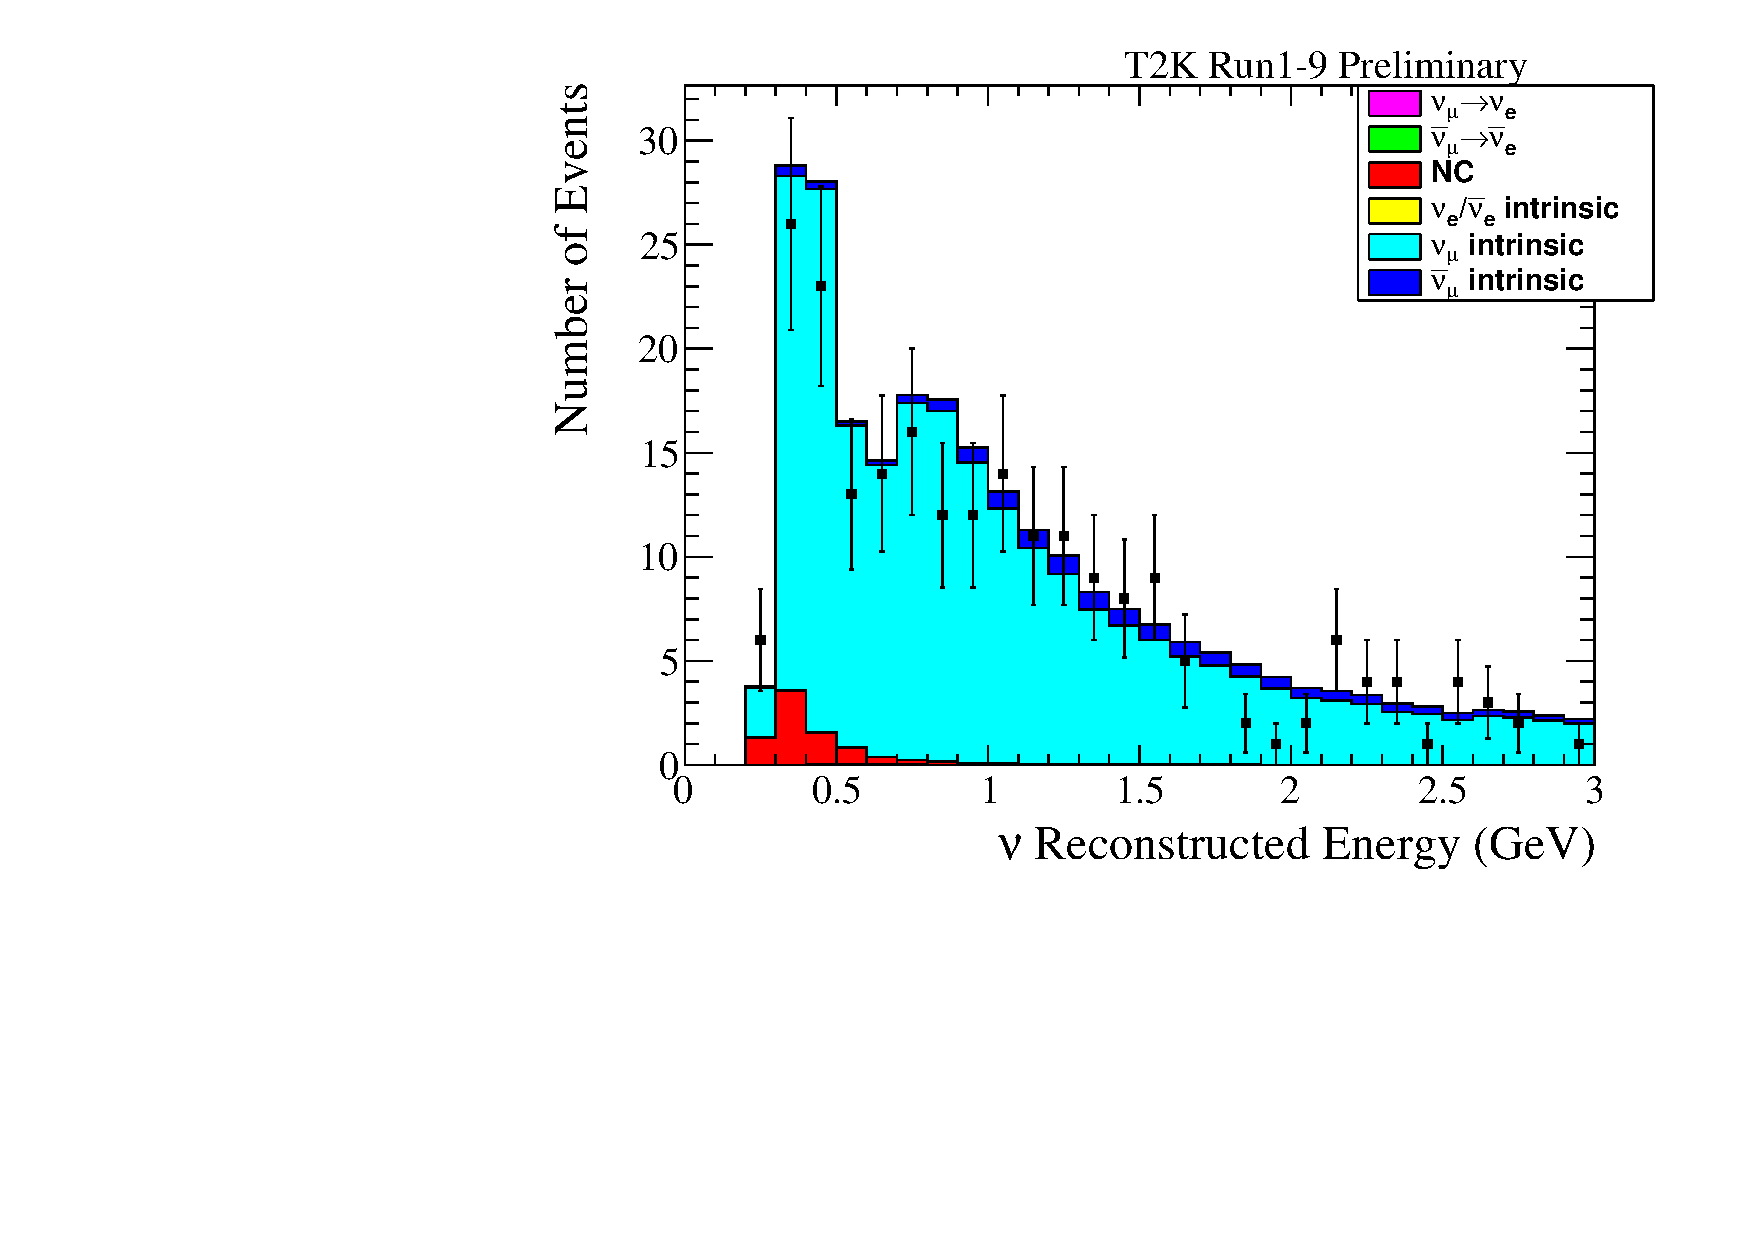
\includegraphics[width=0.9\textwidth]{images/spectra/data/spectrum_asimov_run1-9_1Rmu_data}
		\caption{Muon-like, neutrino mode}
	\end{subfigure}
	\begin{subfigure}[b]{0.49\textwidth}
		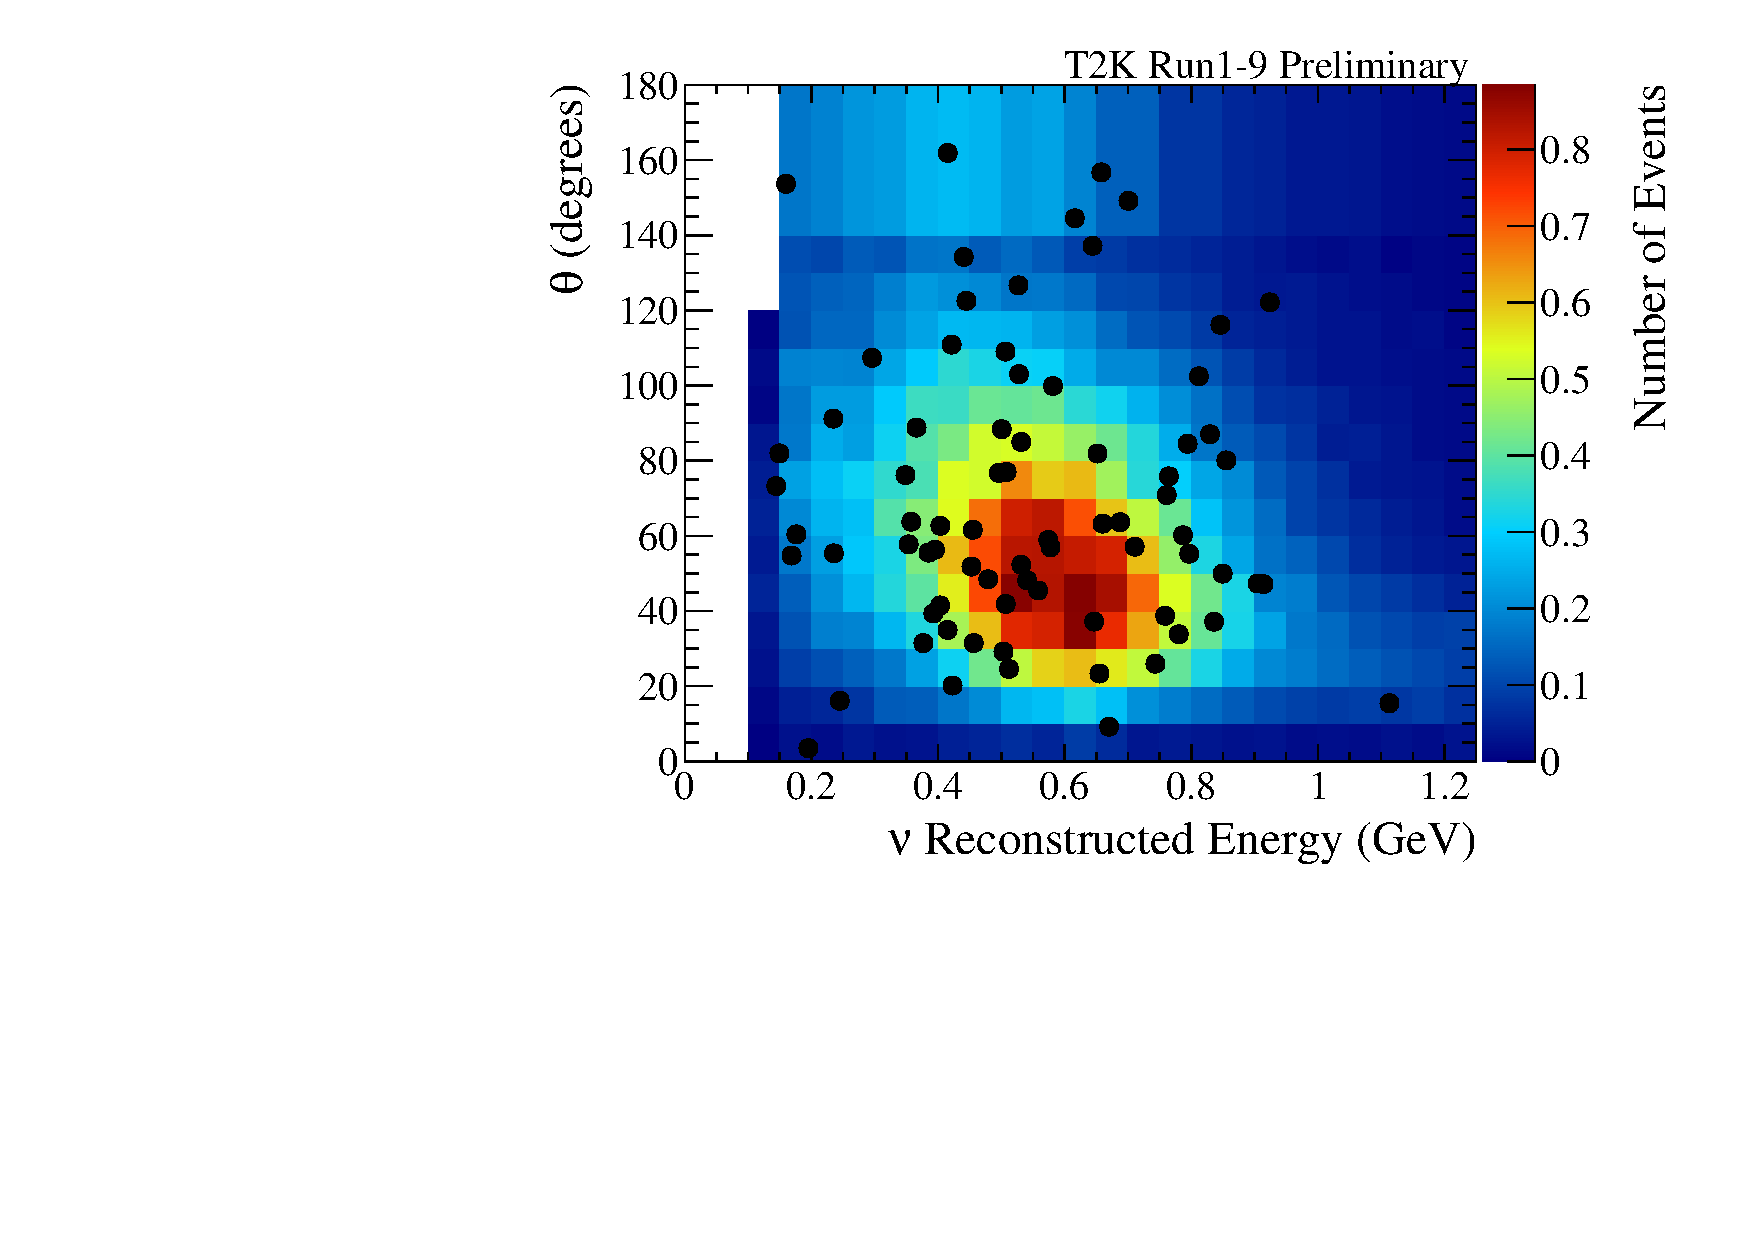
\includegraphics[width=0.9\textwidth]{images/spectra/data/spectrum_asimov_run1-9_1Re_data}
		\caption{Electron-like, neutrino mode}
	\end{subfigure}
	\begin{subfigure}[b]{0.49\textwidth}
		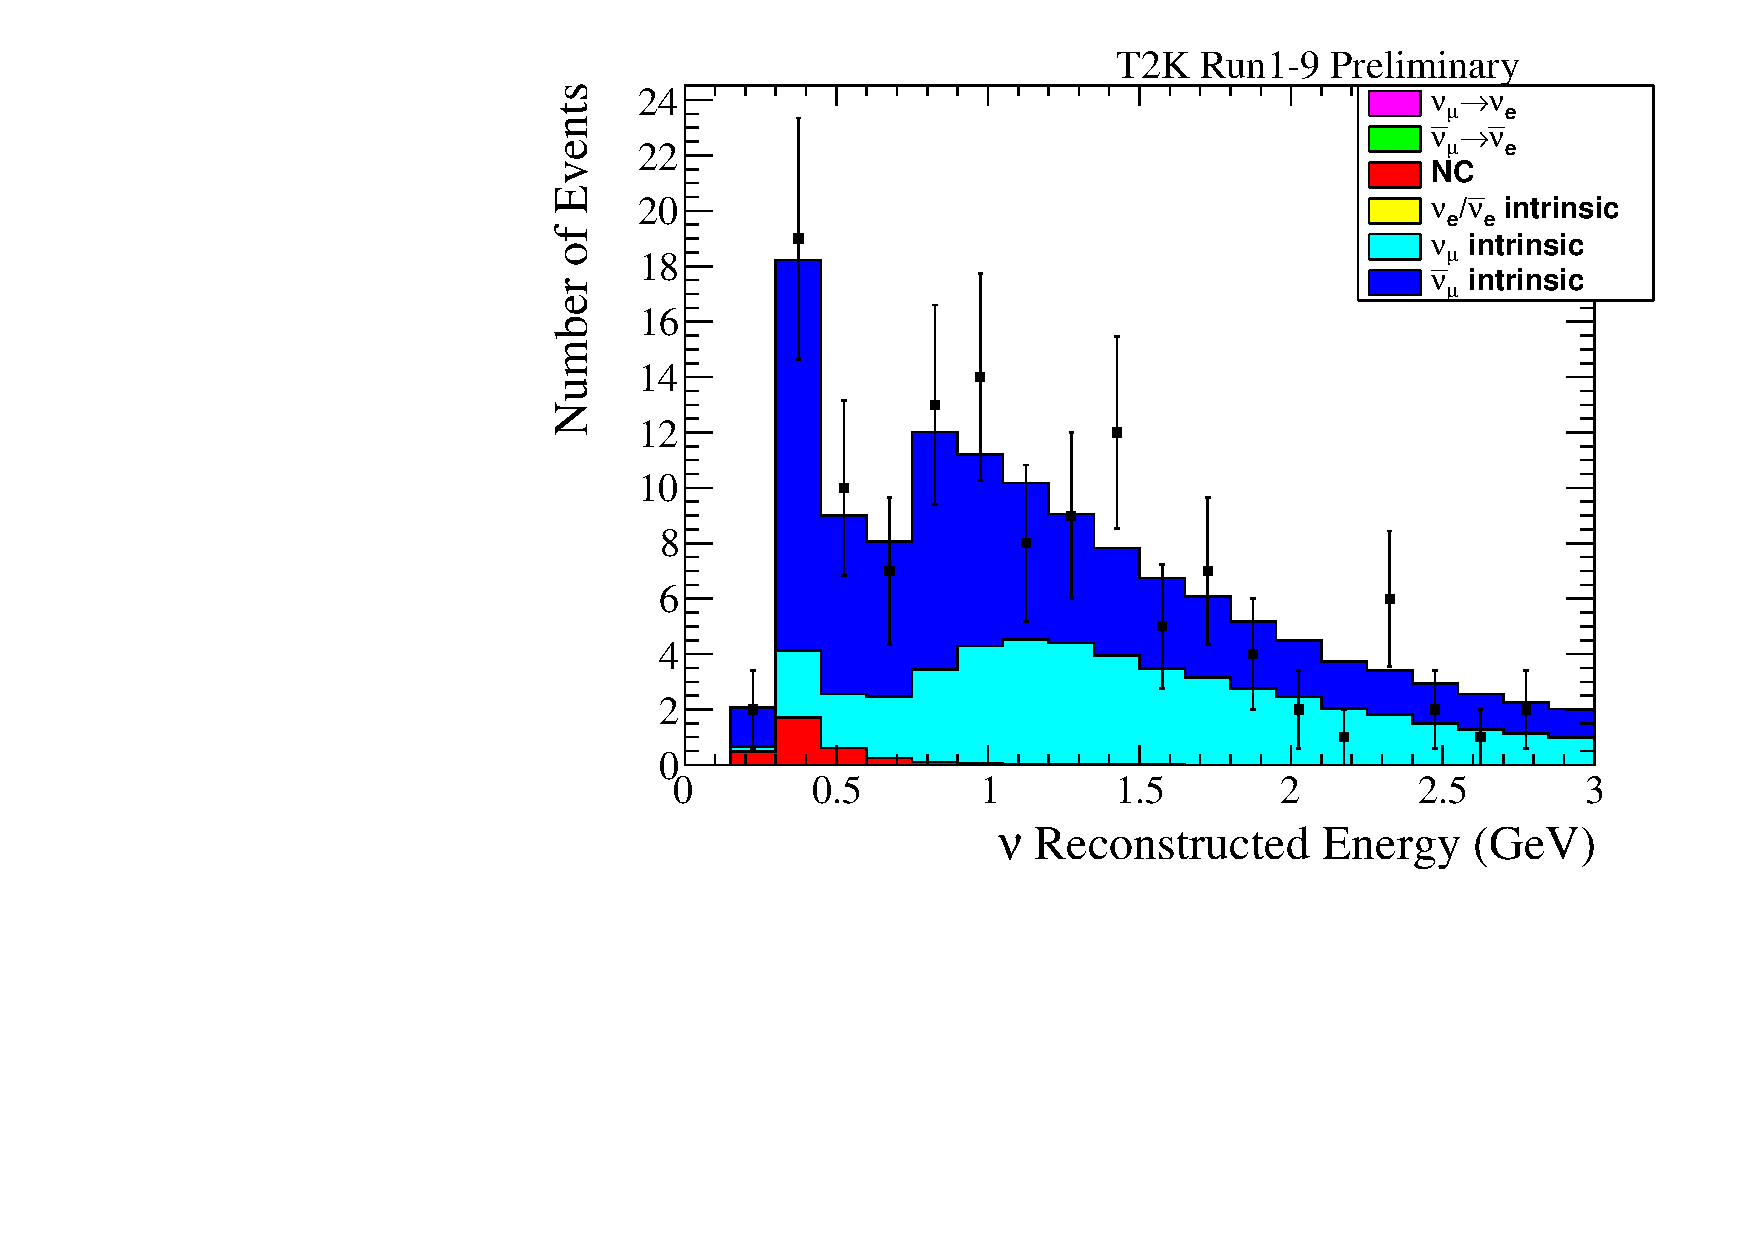
\includegraphics[width=0.9\textwidth]{images/spectra/data/spectrum_asimov_run1-9_RHC1Rmu_data}
		\caption{Muon-like, antineutrino mode}
	\end{subfigure}
	\begin{subfigure}[b]{0.49\textwidth}
		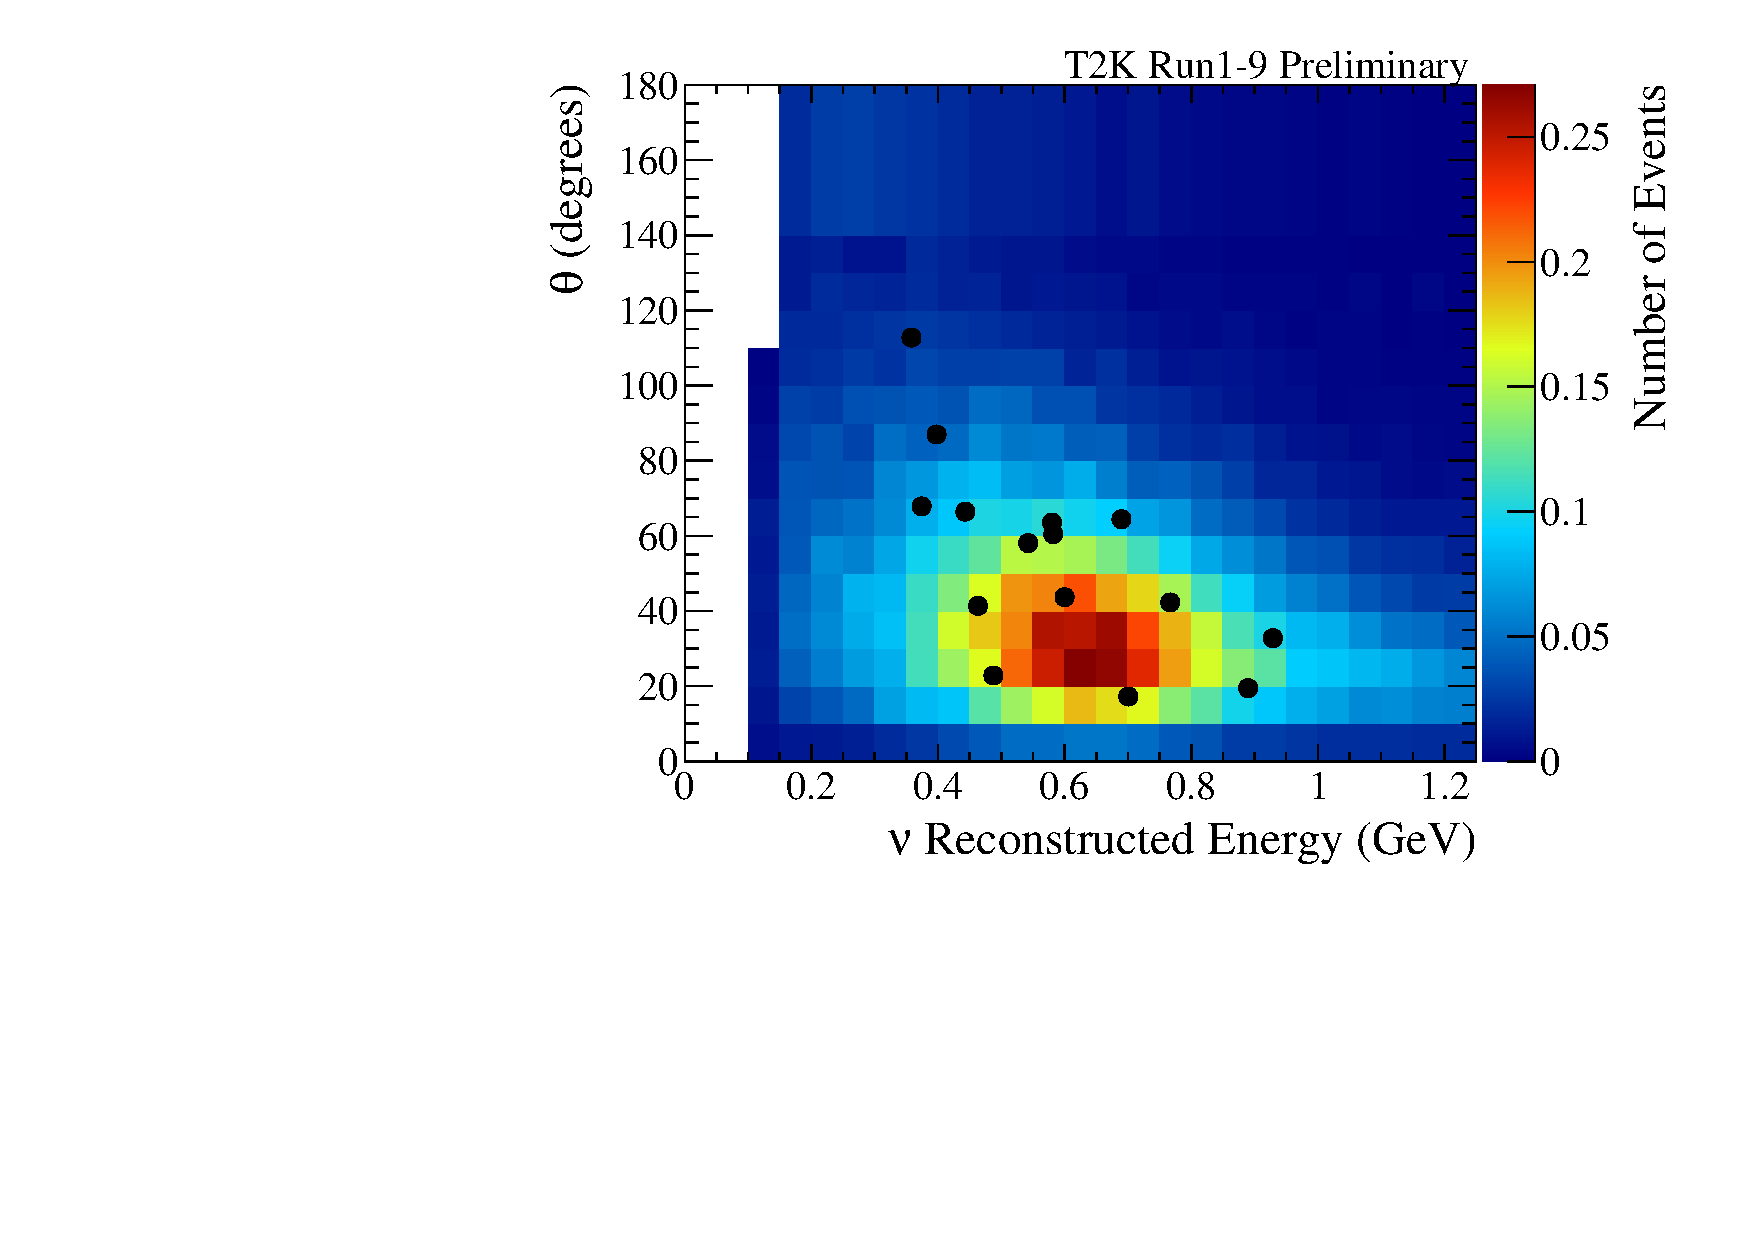
\includegraphics[width=0.9\textwidth]{images/spectra/data/spectrum_asimov_run1-9_RHC1Re_data}
		\caption{Electron-like antineutrino mode}
	\end{subfigure}
	\begin{subfigure}[b]{0.49\textwidth}
		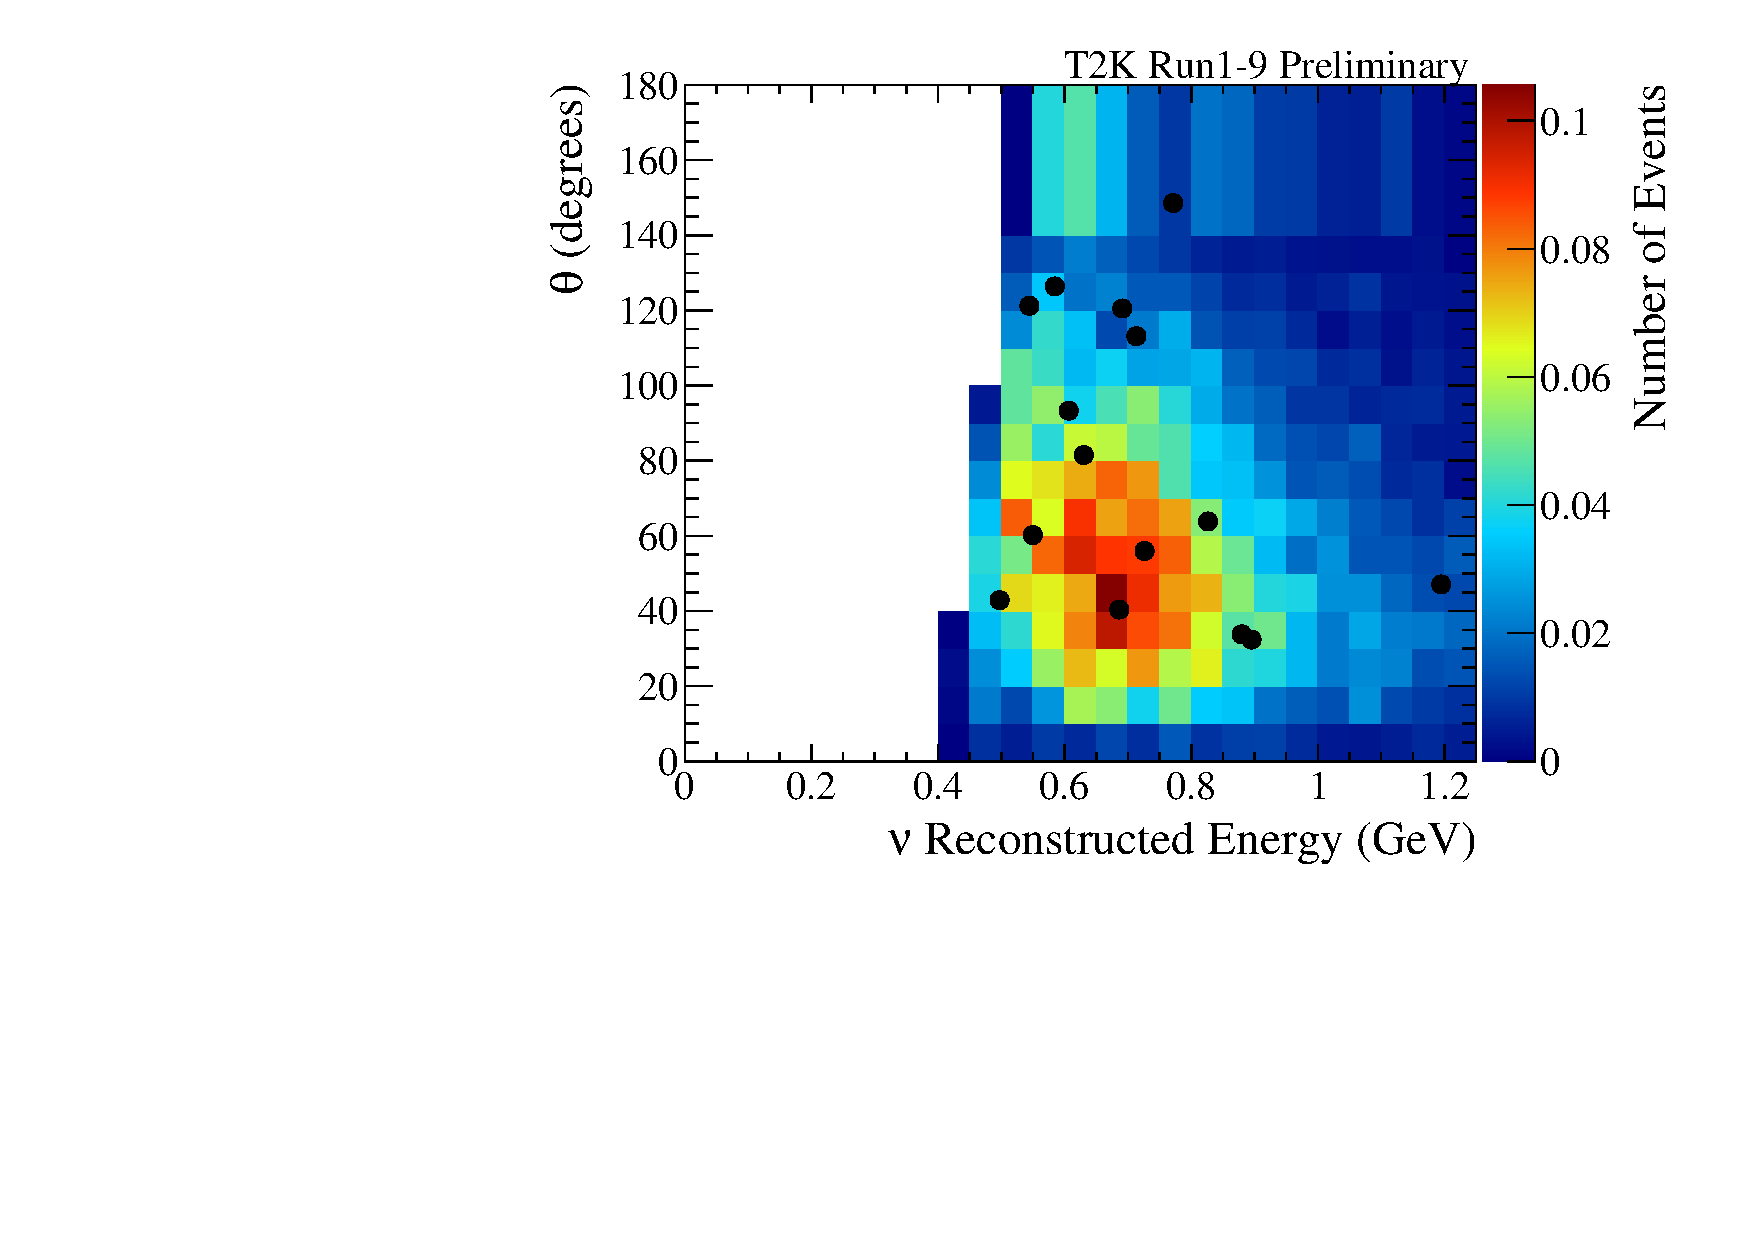
\includegraphics[width=0.9\textwidth]{images/spectra/data/spectrum_asimov_run1-9_MultiRe_data}
		\caption{\nueCConepi-like, neutrino mode}
	\end{subfigure}
	\caption {
		Predicted spectra and observed events (points). $\mu$-like distributions are a function of the reconstructed neutrino energy, while the $e$-like, including \nueCConepi, distributions are functions of both the reconstructed neutrino energy and the reconstructed angle between the outgoing lepton and the neutrino direction. The distributions correspond to the statistics collected in the full \RunPeriod data set. The spectra are generated with the systematic parameters described in \cref{sec:systematics} and the oscillation parameters corresponding to the best-fit values from the data fit (solar parameters at PDG 2016).
	}
	\label{fig:asimovpf_spectra_mc_data}
\end{figure*}
\clearpage
\begin{figure*}[htb]
	\center

	\begin{subfigure}[b]{0.49\textwidth}
		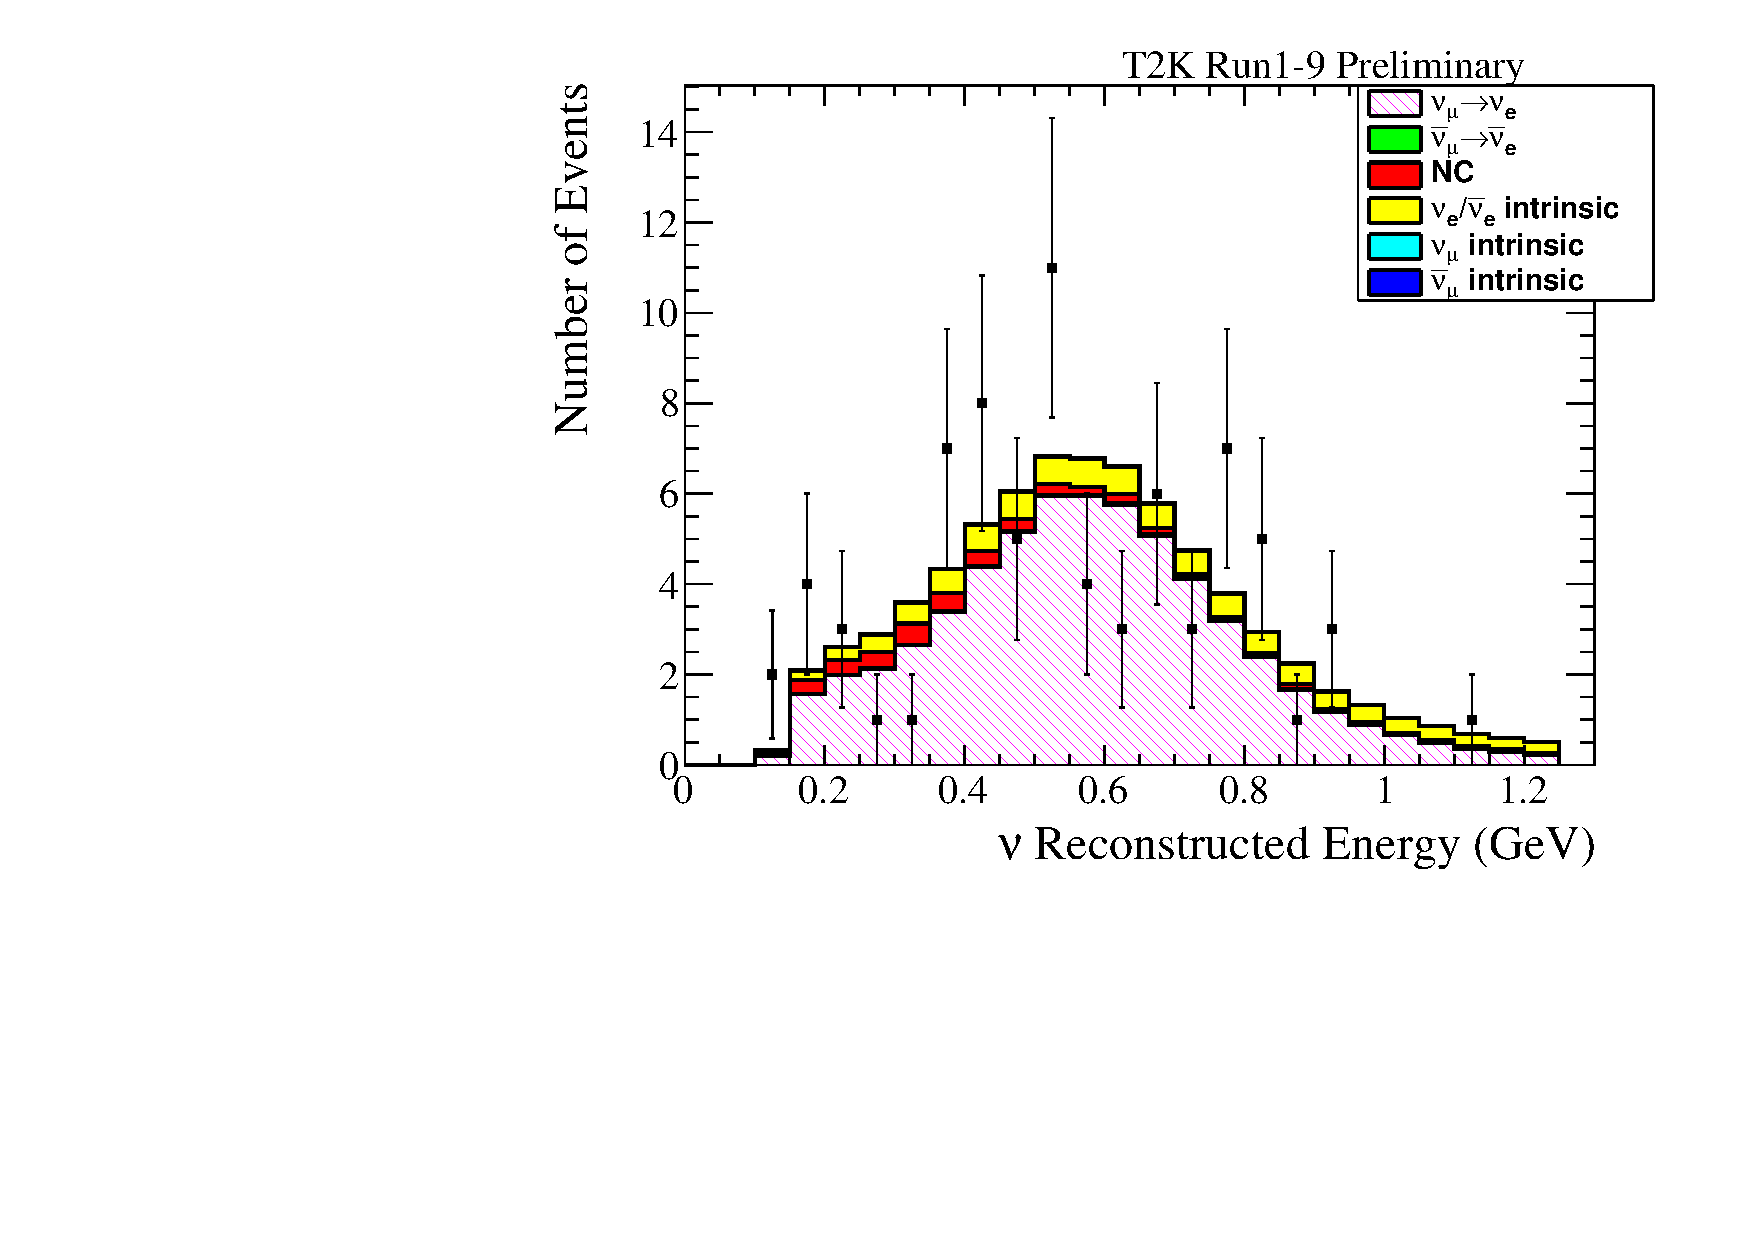
\includegraphics[width=0.9\textwidth]{images/spectra/data/erec_spectrum_asimov_run1-9_1Re_data}
		\caption{Electron-like, neutrino mode}
	\end{subfigure}
	\begin{subfigure}[b]{0.49\textwidth}
		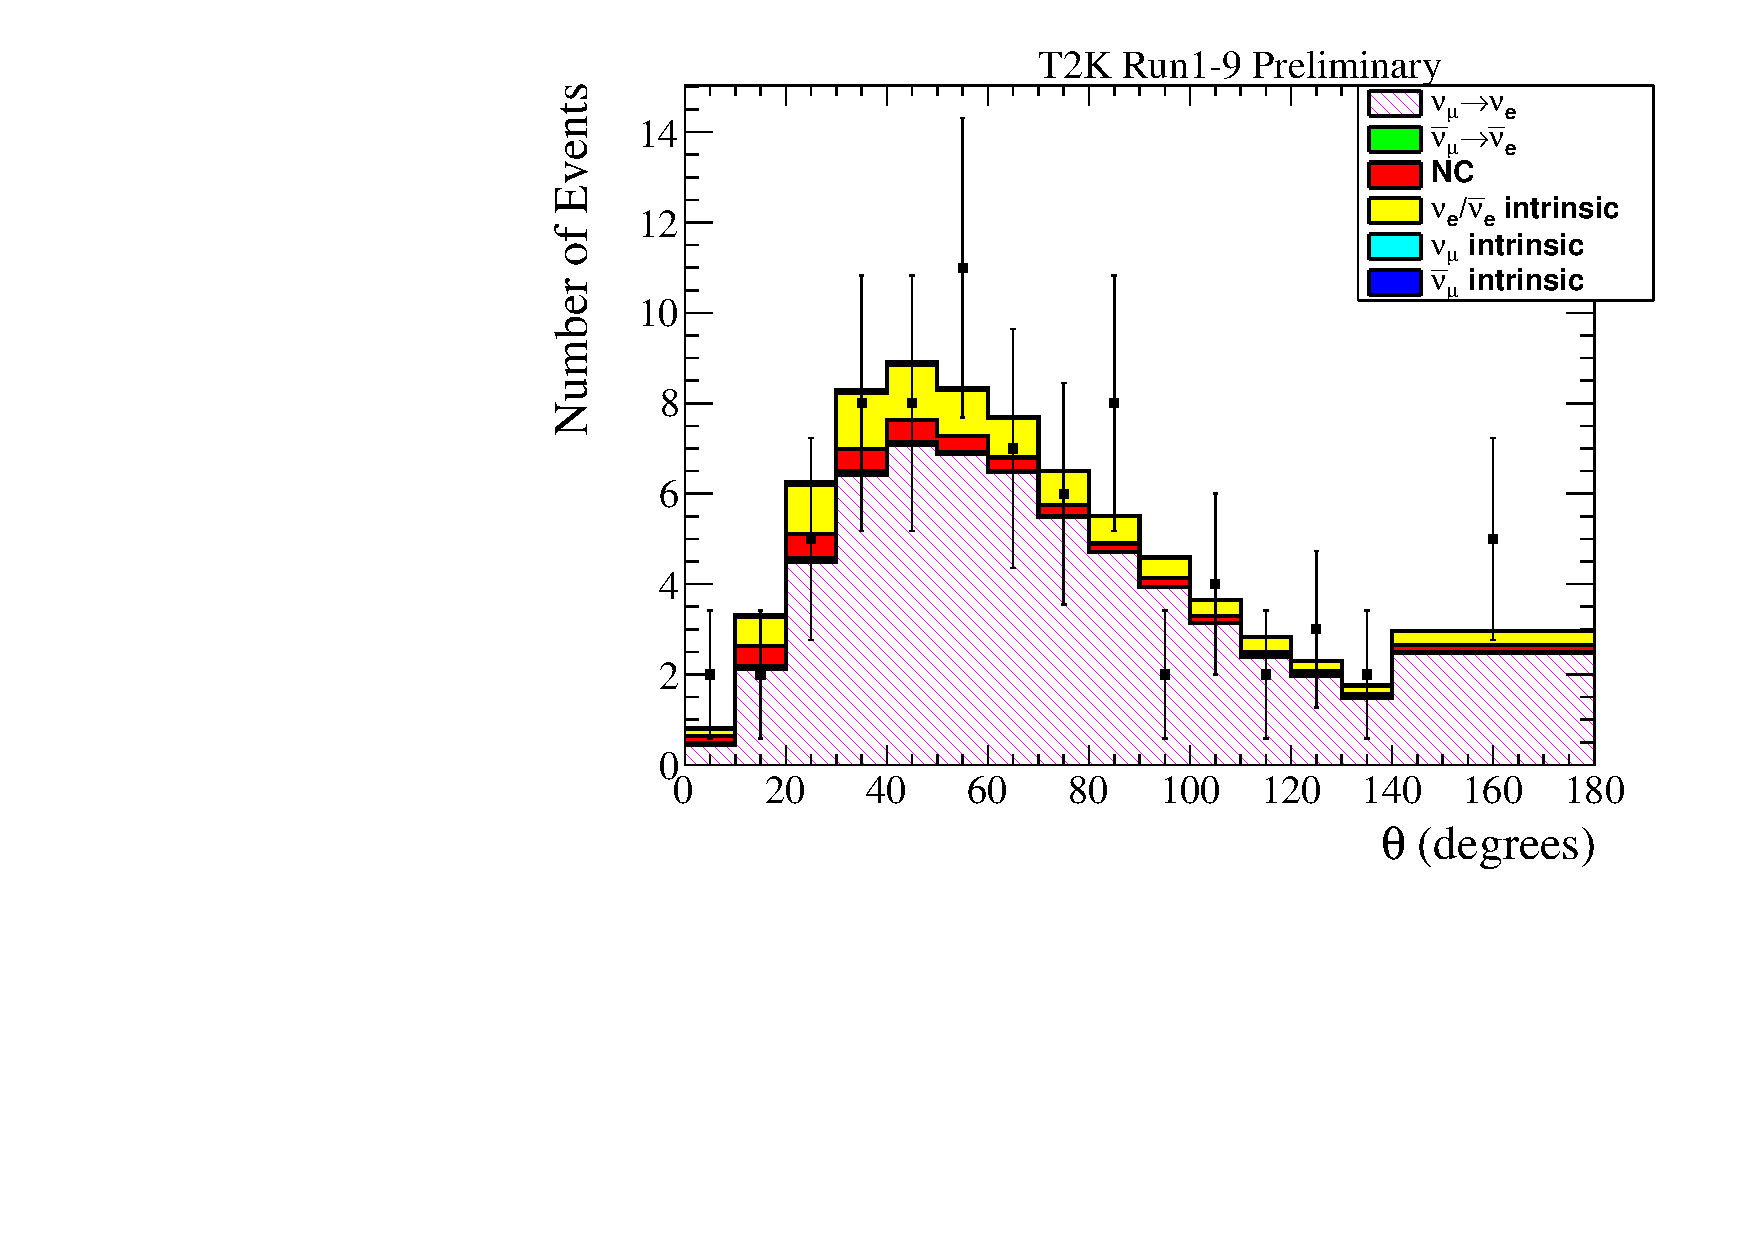
\includegraphics[width=0.9\textwidth]{images/spectra/data/theta_spectrum_asimov_run1-9_1Re_data}
		\caption{Electron-like, neutrino mode}
	\end{subfigure}

	\begin{subfigure}[b]{0.49\textwidth}
		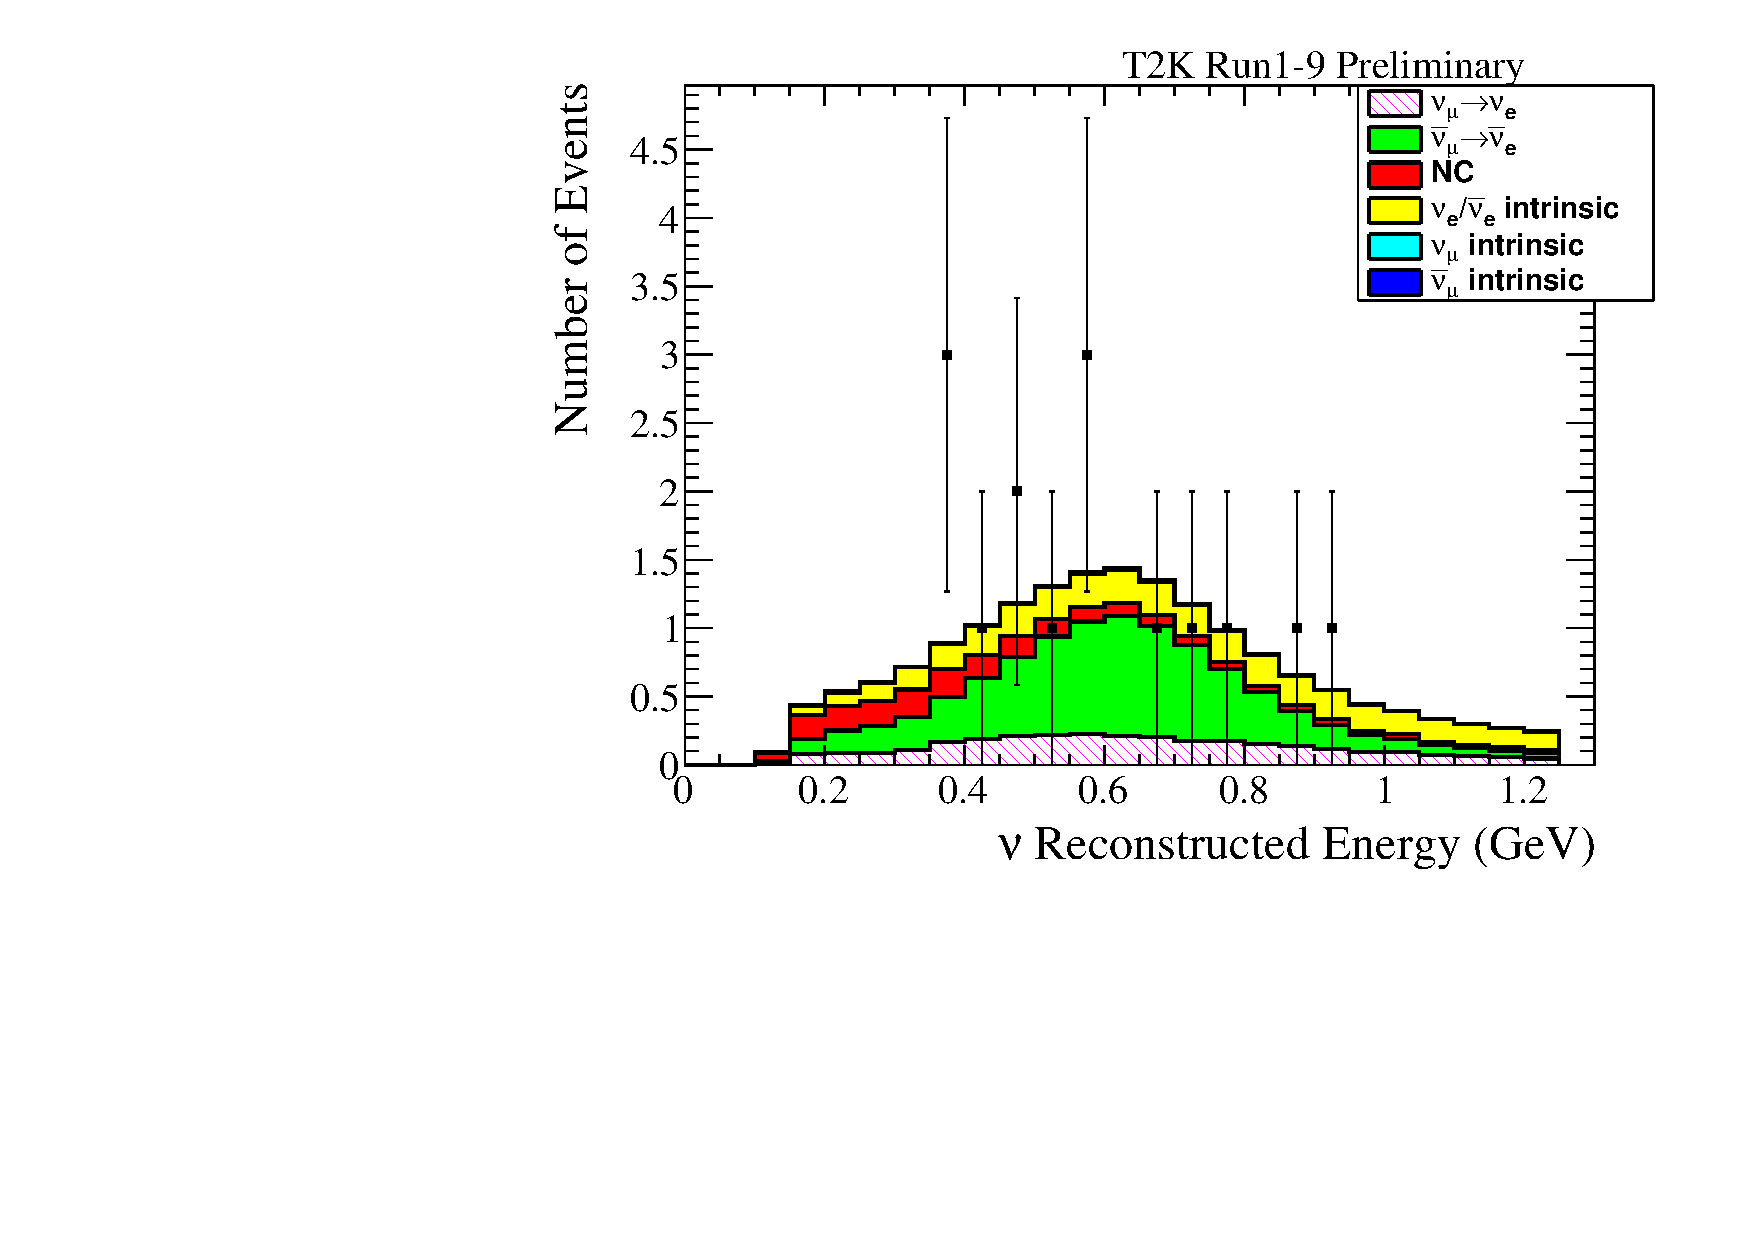
\includegraphics[width=0.9\textwidth]{images/spectra/data/erec_spectrum_asimov_run1-9_RHC1Re_data}
		\caption{Electron-like antineutrino mode}
	\end{subfigure}
	\begin{subfigure}[b]{0.49\textwidth}
		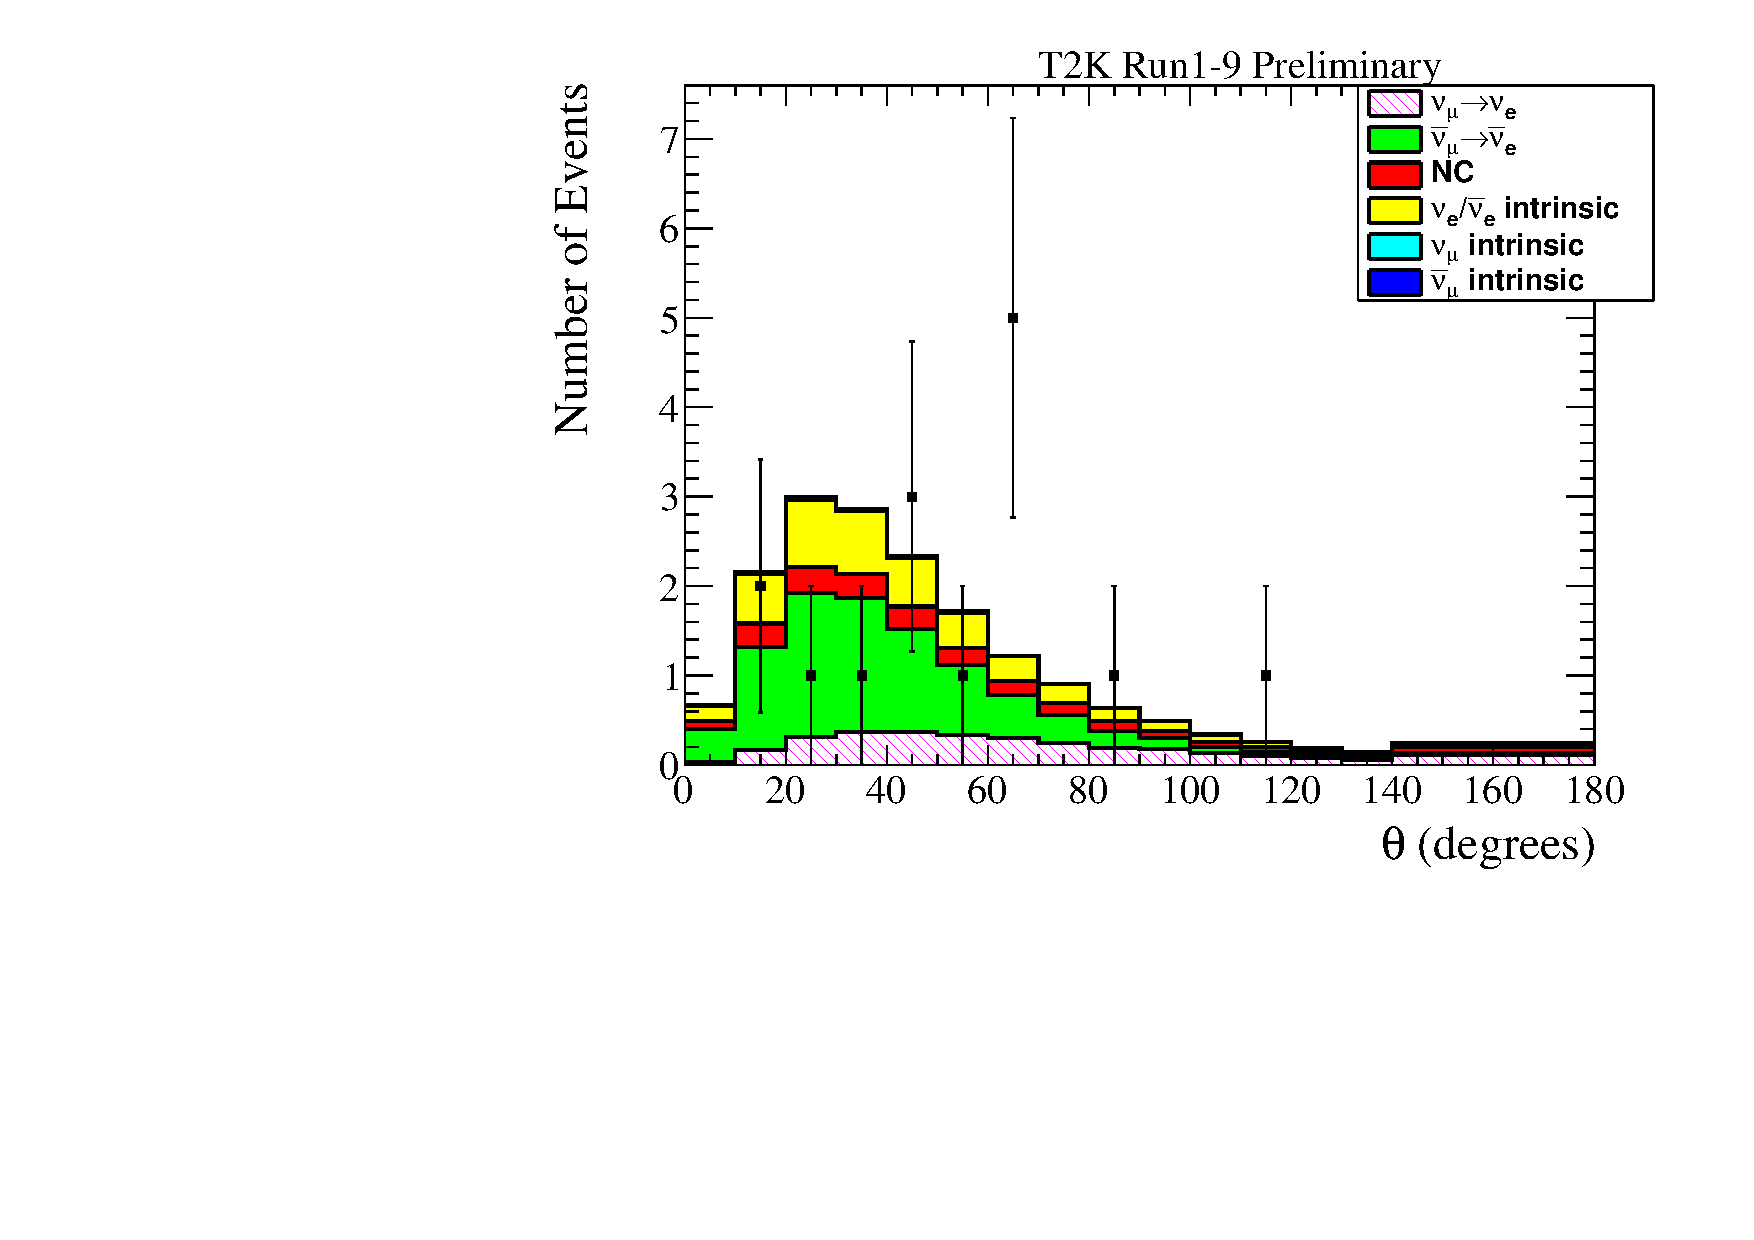
\includegraphics[width=0.9\textwidth]{images/spectra/data/theta_spectrum_asimov_run1-9_RHC1Re_data}
		\caption{Electron-like antineutrino mode}
	\end{subfigure}

	\begin{subfigure}[b]{0.49\textwidth}
		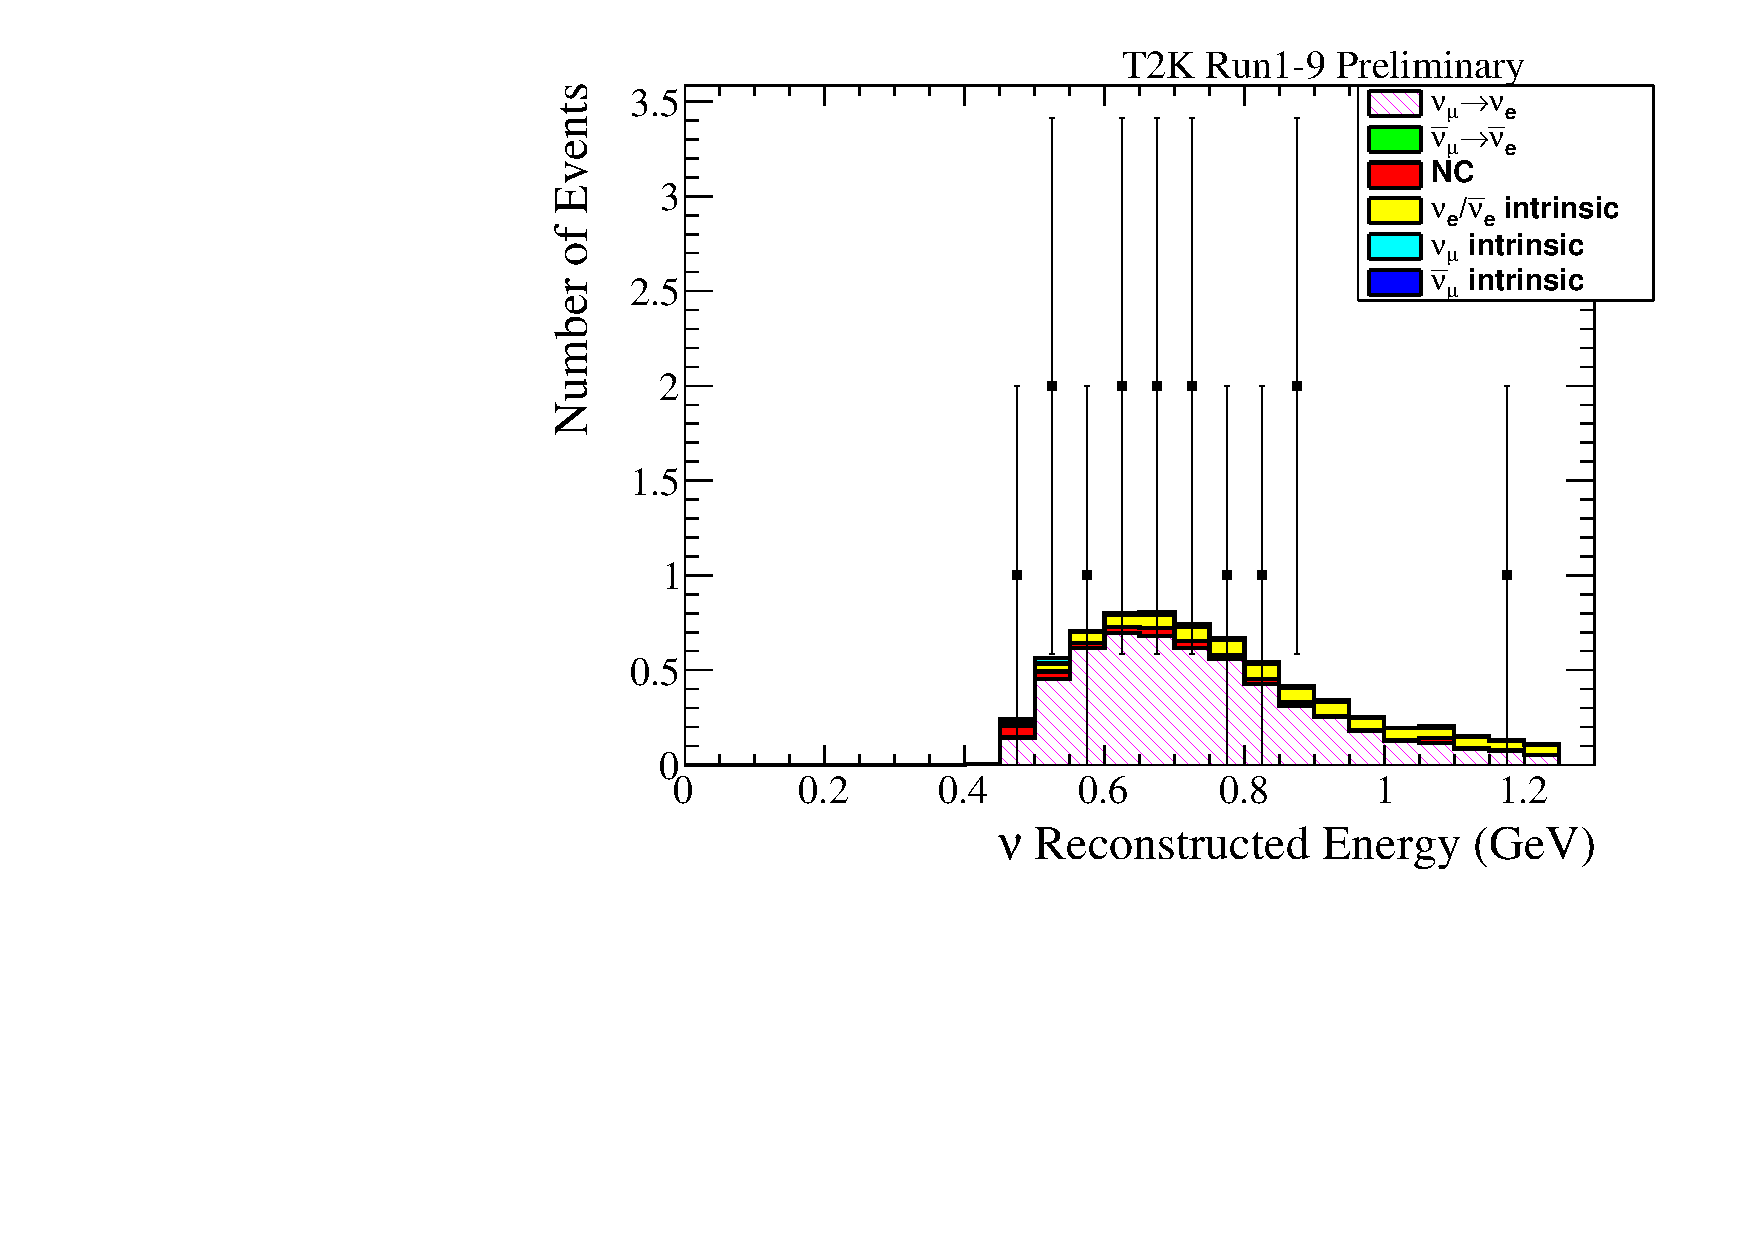
\includegraphics[width=0.9\textwidth]{images/spectra/data/erec_spectrum_asimov_run1-9_MultiRe_data}
		\caption{\nueCConepi-like, neutrino mode}
	\end{subfigure}
	\begin{subfigure}[b]{0.49\textwidth}
		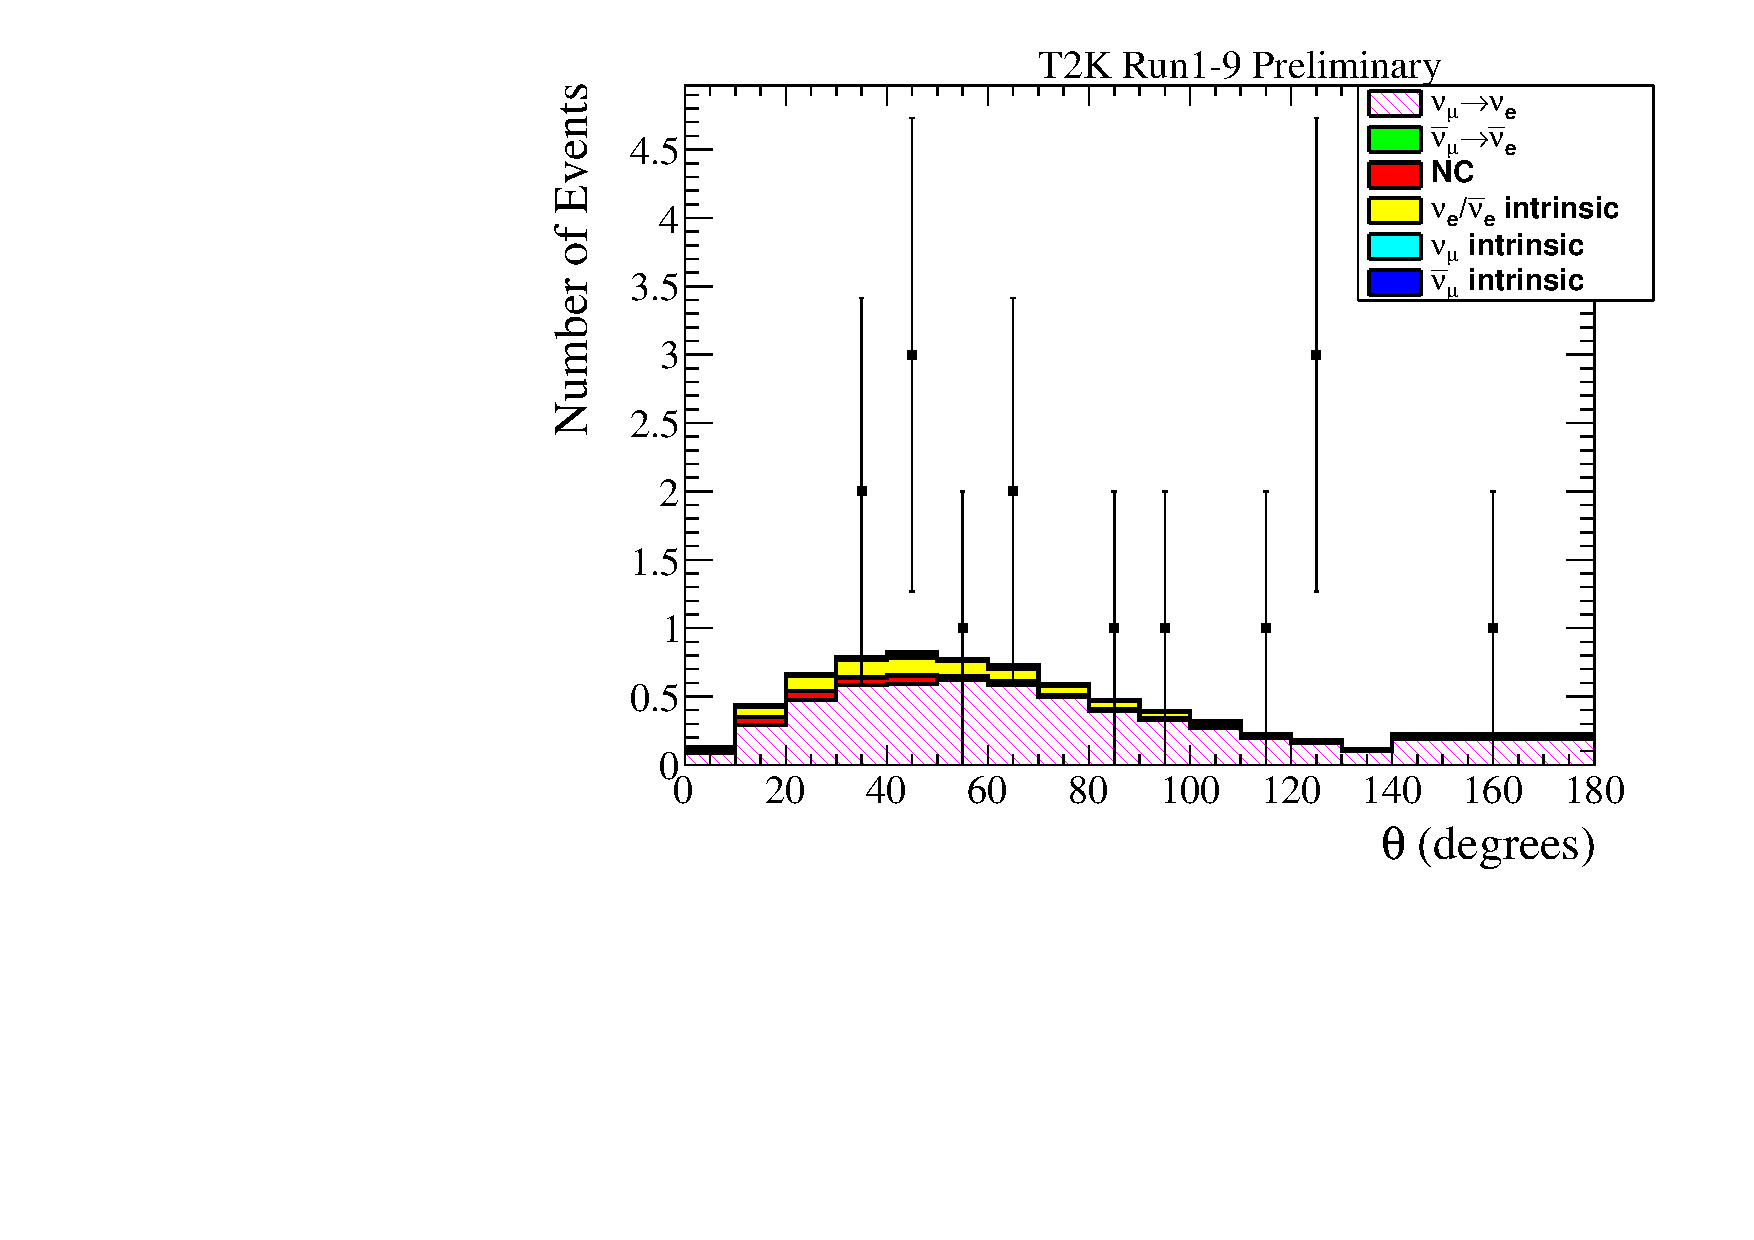
\includegraphics[width=0.9\textwidth]{images/spectra/data/theta_spectrum_asimov_run1-9_MultiRe_data}
		\caption{\nueCConepi-like, neutrino mode}
	\end{subfigure}
	\caption {
		Predicted spectra and observed events (points). The $e$-like, including \nueCConepi, distributions are functions of both the reconstructed neutrino energy and the reconstructed angle between the outgoing lepton and the neutrino direction, with the projections in each variable shown here. The distributions correspond to the statistics collected in the full \RunPeriod data set. The spectra are generated with the systematic parameters described in \cref{sec:systematics} and the oscillation parameters corresponding to the best-fit values from the data fit (solar parameters at PDG 2016).
	}
	\label{fig:asimovpf_spectra_mc_data_elike_1D}
\end{figure*}
\clearpage

The best-fit values and $1\sigma$ ranges for each oscillation parameter are shown in \cref{tab:data_bestfit} for normal hierarchy (which is preferred in all data fits) and inverted hierarchy (local interval). The $1\sigma$ ranges are extracted for each oscillation parameter from the 1-dimensional $\Delta \chi^2$ distributions shown in \crefrange{fig:dcp_data}{fig:dmsq23_data}.

The 1-dimensional contours are plotted with respect to the global minimum from normal and inverted hierarchies, while the 2-dimensional confidence intervals are shown drawing the normal and inverted hierarchy contours independently, i.e. each contour is produced with respect to the global minimum under that hierarchy hypothesis.

For \deltacp, the reactor measurements are in agreement with T2K-only data at the $1\sigma$ level.

\begin{table}
\centering
\begin{tabular}{| c | c | c | c | c | c |}
\hline
Parameter & Reactor & Best-fit (NH) & $\pm1\sigma$ (NH) & Best-fit (IH) & $\pm1\sigma$ (IH) \\
\hline
\deltacp & Yes & \BestFitDeltacpwRC & [\MOneSigmaDeltacpwRC,\POneSigmaDeltacpwRC] & \BestFitDeltacpwRCIH & [\MOneSigmaDeltacpwRCIH,\POneSigmaDeltacpwRCIH] \\
\deltacp & No & \BestFitDeltacpwoRC & [\MOneSigmaDeltacpwoRC,\POneSigmaDeltacpwoRC] & \BestFitDeltacpwoRCIH & [\MOneSigmaDeltacpwoRCIH,\POneSigmaDeltacpwoRCIH] \\
\ssqthonethree & No & \BestFitMixingOneThreewoRC & [\MOneMixingOneThreewoRC,\POneMixingOneThreewoRC] & \BestFitMixingOneThreewoRCIH & [\MOneMixingOneThreewoRCIH,\POneMixingOneThreewoRCIH] \\
\ssqthtwothree & Yes & \BestFitMixingTwoThreewRC & [\MOneMixingTwoThreewRC,\POneMixingTwoThreewRC] & \BestFitMixingTwoThreewRCIH & [\MOneMixingTwoThreewRCIH,\POneMixingTwoThreewRCIH] \\
\dmsqtwothree or \dmsqonethree & Yes & \BestFitDmTwoThreewRC & [\MOneDmTwoThreewRC,\POneDmTwoThreewRC] & \BestFitDmTwoThreewRCIH & [\MOneDmTwoThreewRCIH,\POneDmTwoThreewRCIH] \\
 ($10^{-3}\text{ eV}^2\text{/c}^4$) & & & & & \\
\hline
\end{tabular}

\caption{
The \RunPeriod measured oscillation parameter best-fit and the $\pm 1\sigma$ intervals are shown for normal and inverted hierarchies with respect to the hierarchy best-fit. The $\pm 1\sigma$ interval is obtained by using the constant $\Delta \chi^2$ method. For each parameter normal hierarchy is the global best-fit.
}
\label{tab:data_bestfit}
\end{table}
\clearpage

\subsection{Results for \main}
In \cref{fig:dcp_vs_ssqth23_data} the result for \main with reactor constraint and T2K only is shown.

\begin{figure*}[htb]
	\center
	\begin{subfigure}[b]{0.49\textwidth}
		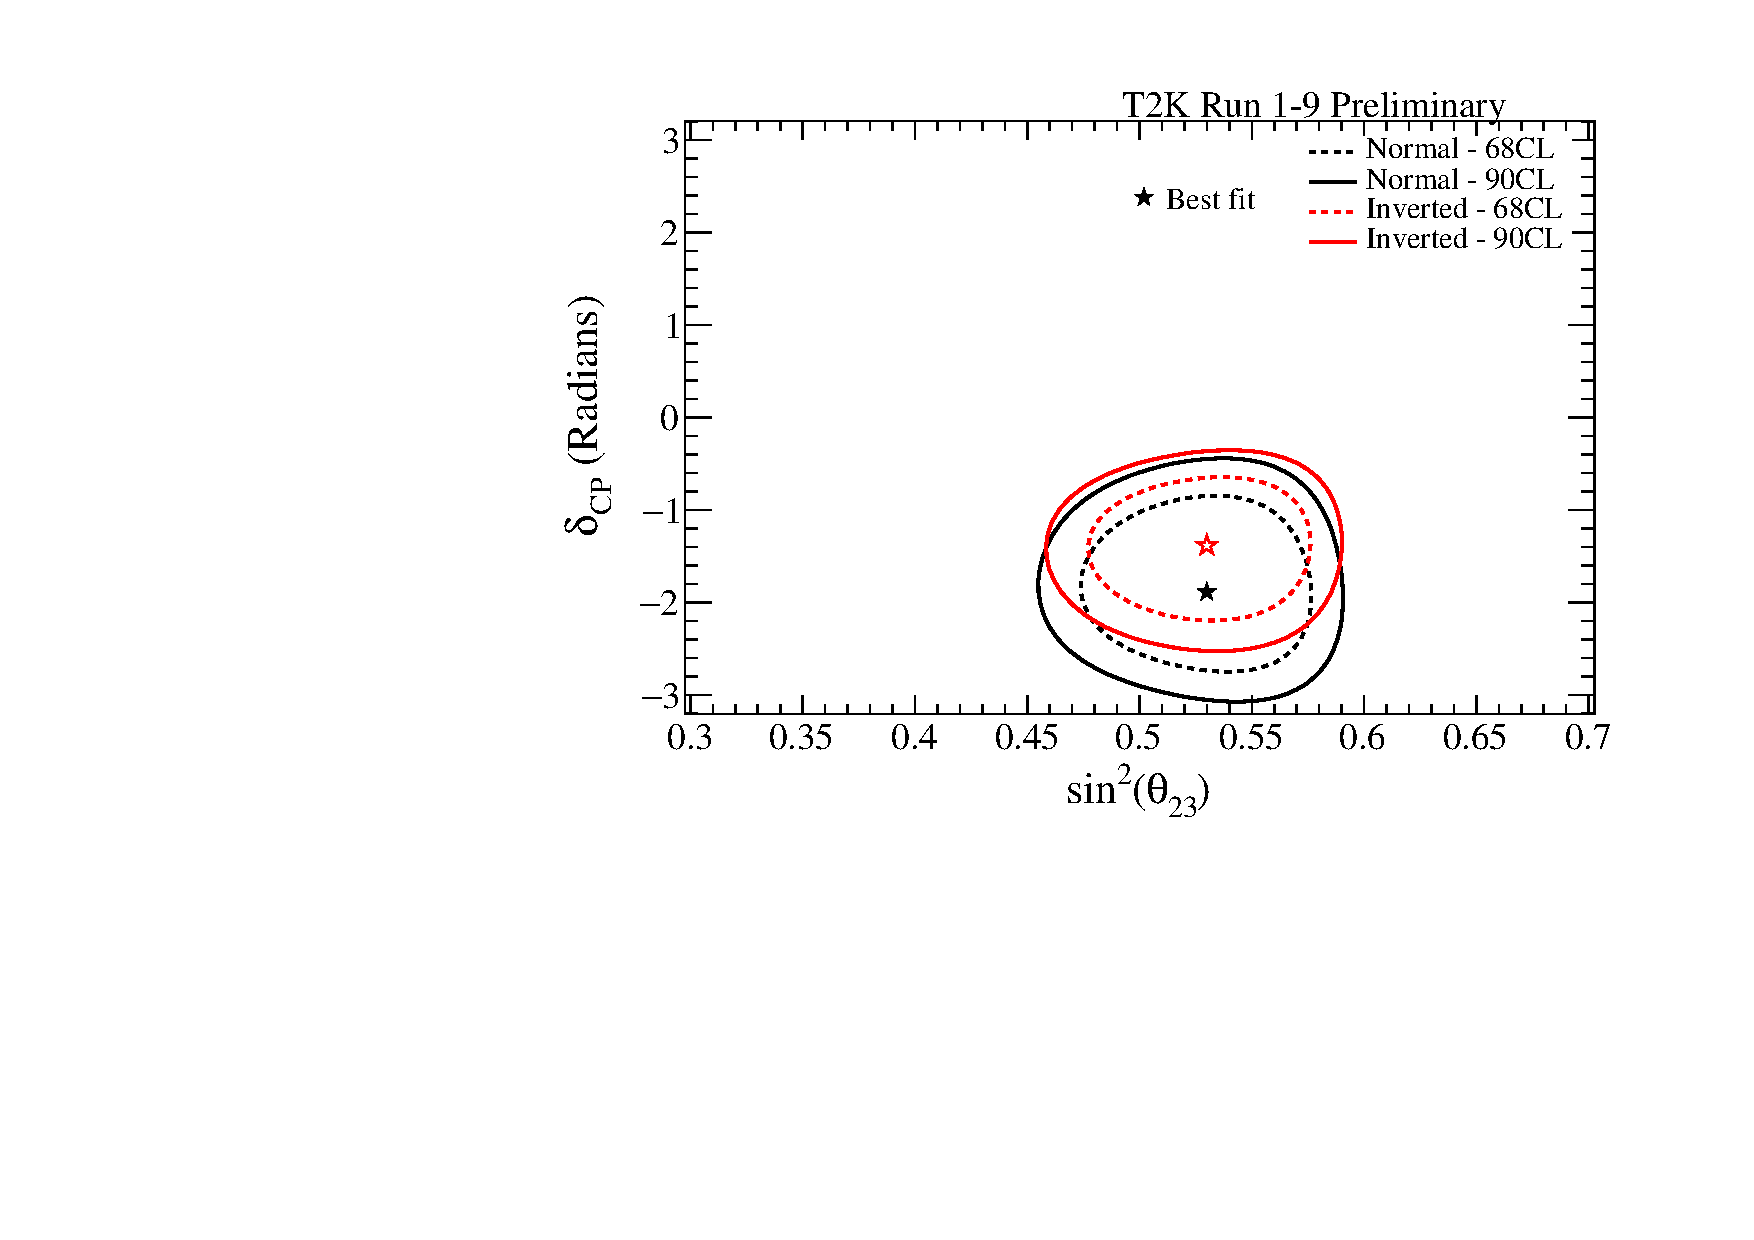
\includegraphics[width=0.9\textwidth]{images/data/mixing23_deltacp_data_reactor_global}
		\caption{\main with reactor constraint}
	\end{subfigure}
	\begin{subfigure}[b]{0.49\textwidth}
		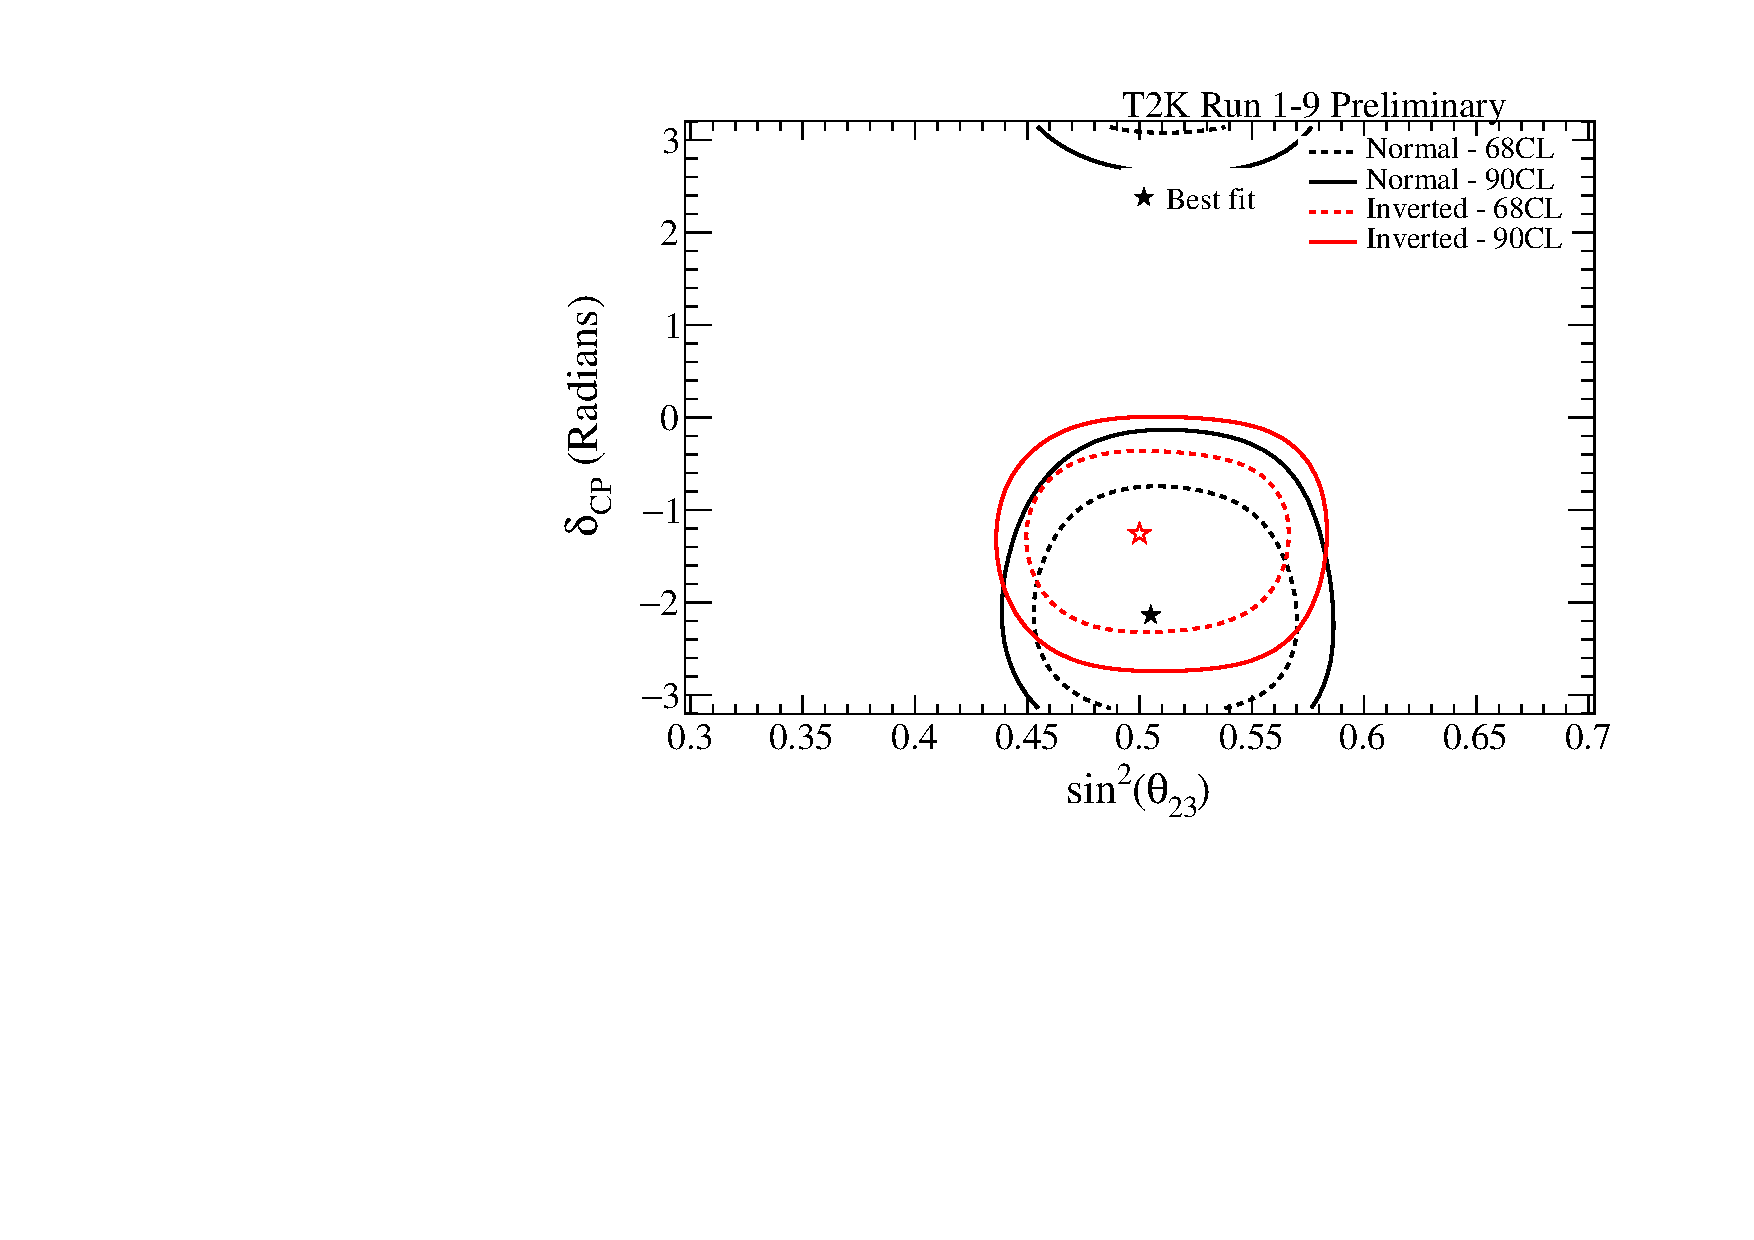
\includegraphics[width=0.9\textwidth]{images/data/mixing23_deltacp_data_t2k_global}
		\caption{\main T2K only}
	\end{subfigure}
	\caption {
		Contours at 68\% and 90\% CL for \main with and without reactor constraint. Normal and inverted hierarchy contours are independent. All 5 samples were used to produce these fits.
	}
	\label{fig:dcp_vs_ssqth23_data}
\end{figure*}

\subsection{Results for \appearance}
In \cref{fig:ssqth13_vs_dcp_data} the result for \appearance with reactor constraint and T2K only is shown.

\begin{figure*}[htb]
	\center
	\begin{subfigure}[b]{0.49\textwidth}
		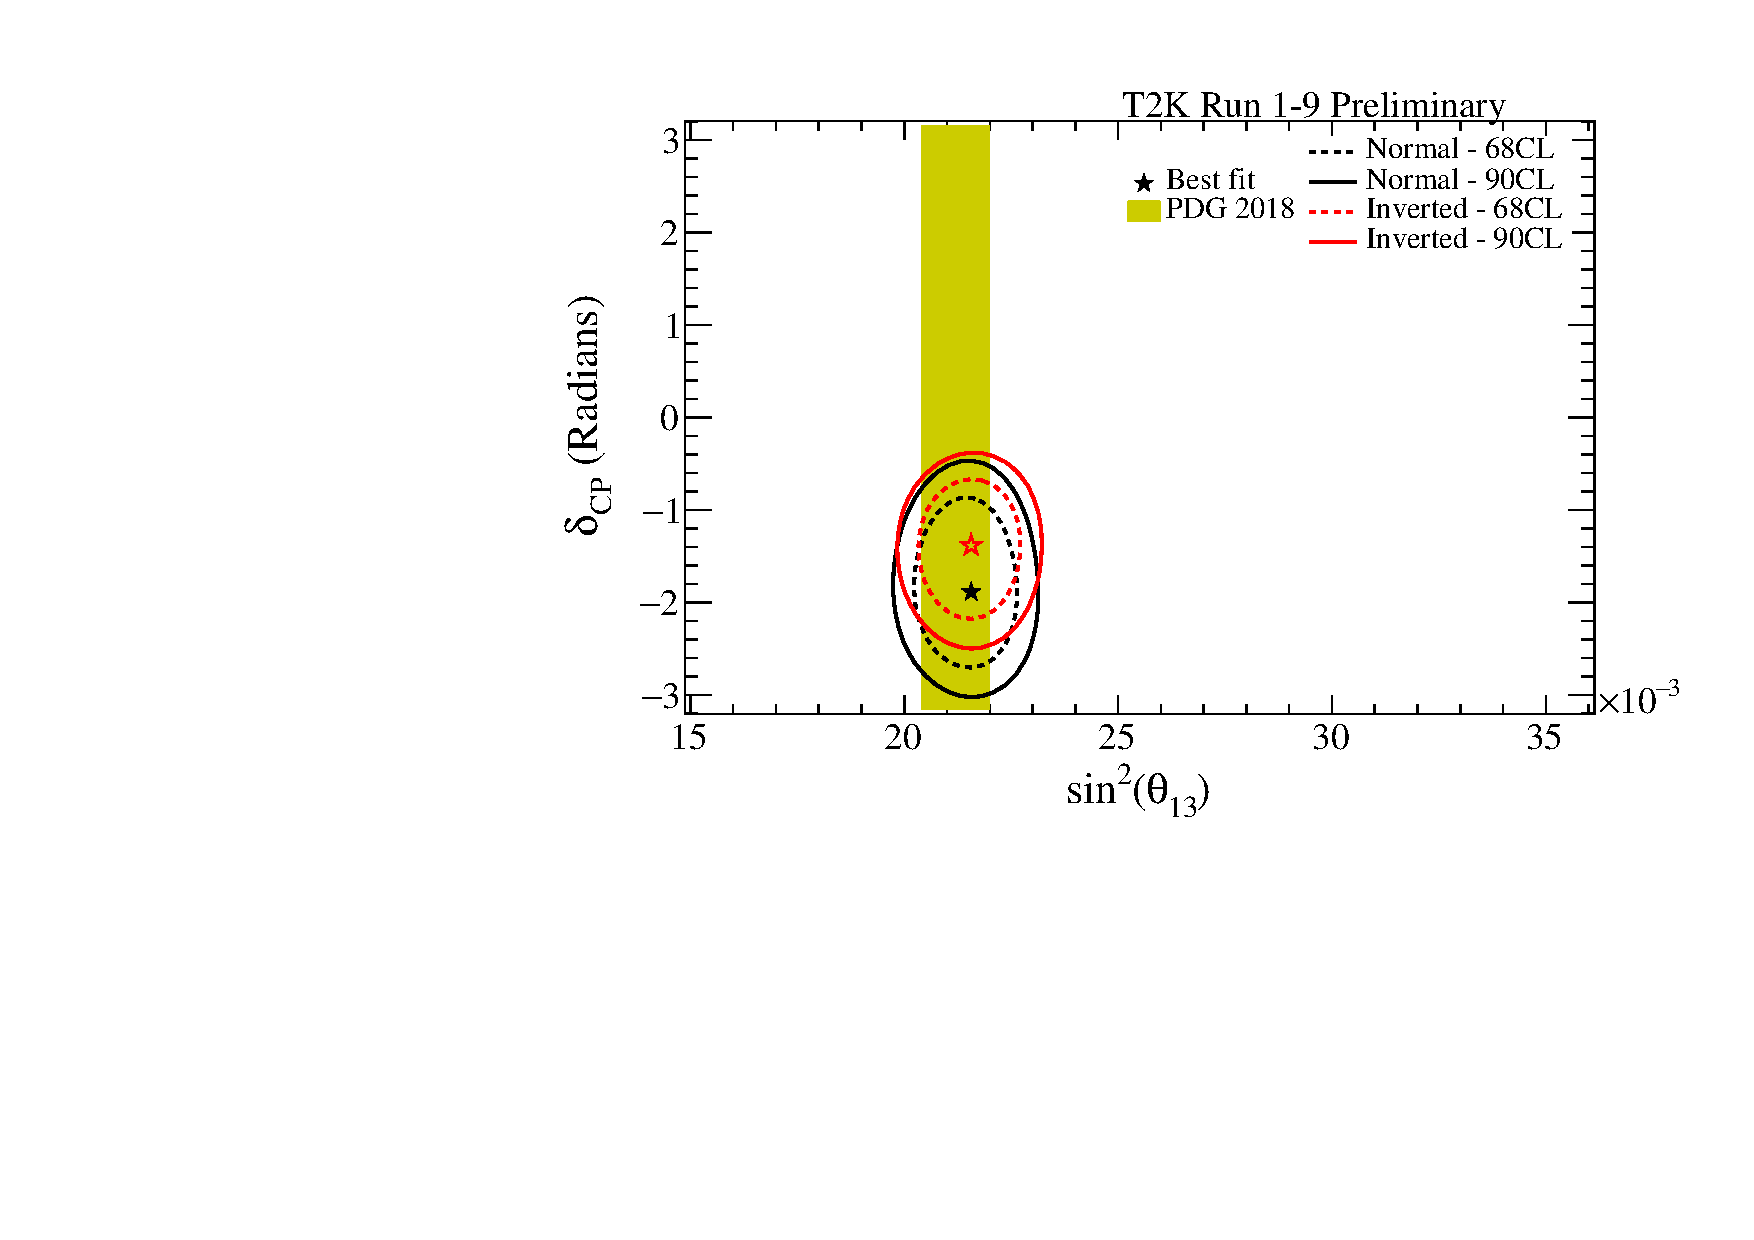
\includegraphics[width=0.9\textwidth]{images/data/mixing13_deltacp_data_reactor_global}
		\caption{\appearance with reactor constraint}
	\end{subfigure}
	\begin{subfigure}[b]{0.49\textwidth}
		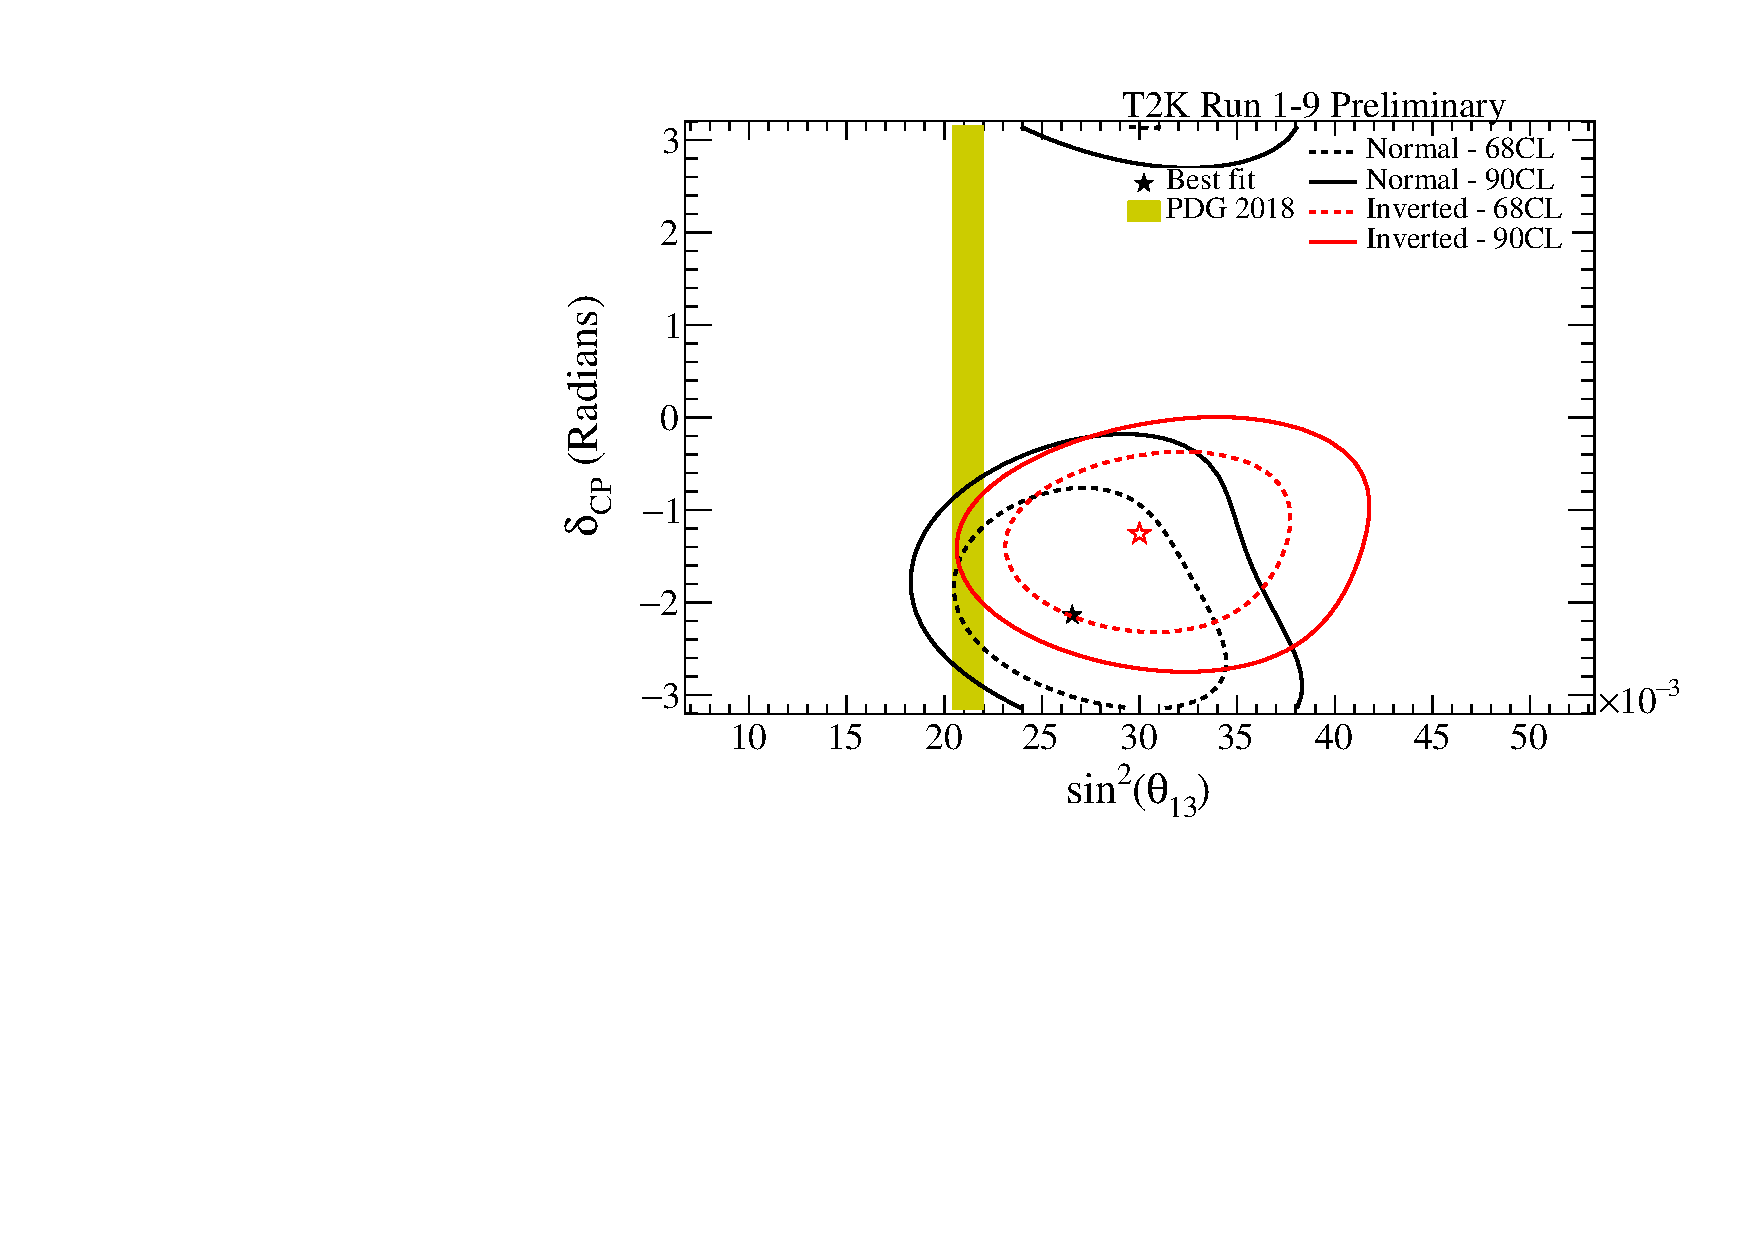
\includegraphics[width=0.9\textwidth]{images/data/mixing13_deltacp_data_t2k_global}
		\caption{\appearance T2K only}
	\end{subfigure}
	\caption {
		Contours at 68\% and 90\% CL for \appearance with and without reactor constraint. Normal and inverted hierarchy contours are independent. All 5 samples were used to produce these fits.
	}
	\label{fig:ssqth13_vs_dcp_data}
\end{figure*}

\clearpage

\subsection{Results for \disappearance}

The result for \disappearance with reactor constraint and T2K only is shown in fig.~\ref{fig:ssqth23_vs_dmsq23_data}.

\begin{figure*}[htb]
	\center
	\begin{subfigure}[b]{0.49\textwidth}
		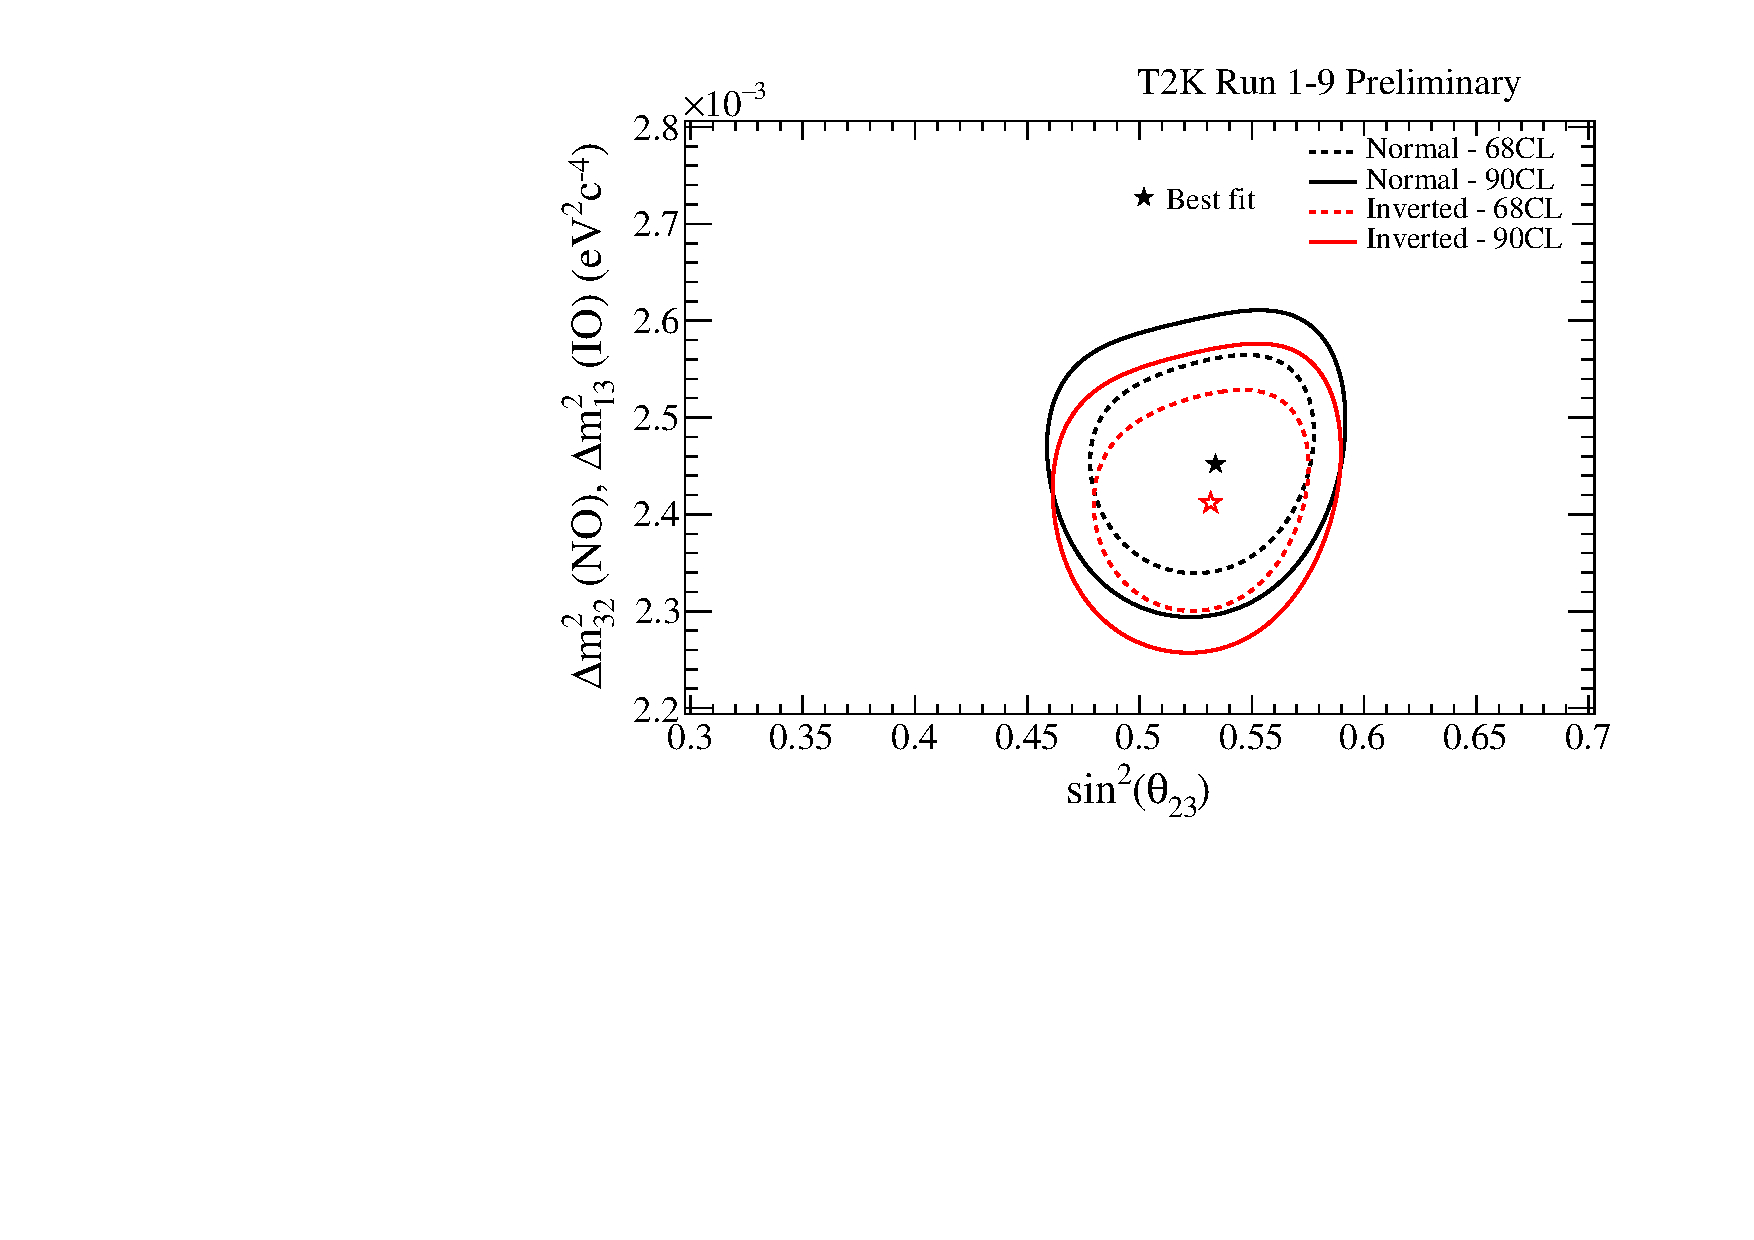
\includegraphics[width=0.9\textwidth]{images/data/mixing23_dmsq23_data_reactor_global}
		\caption{\disappearance with reactor constraint}
	\end{subfigure}
	\begin{subfigure}[b]{0.49\textwidth}
		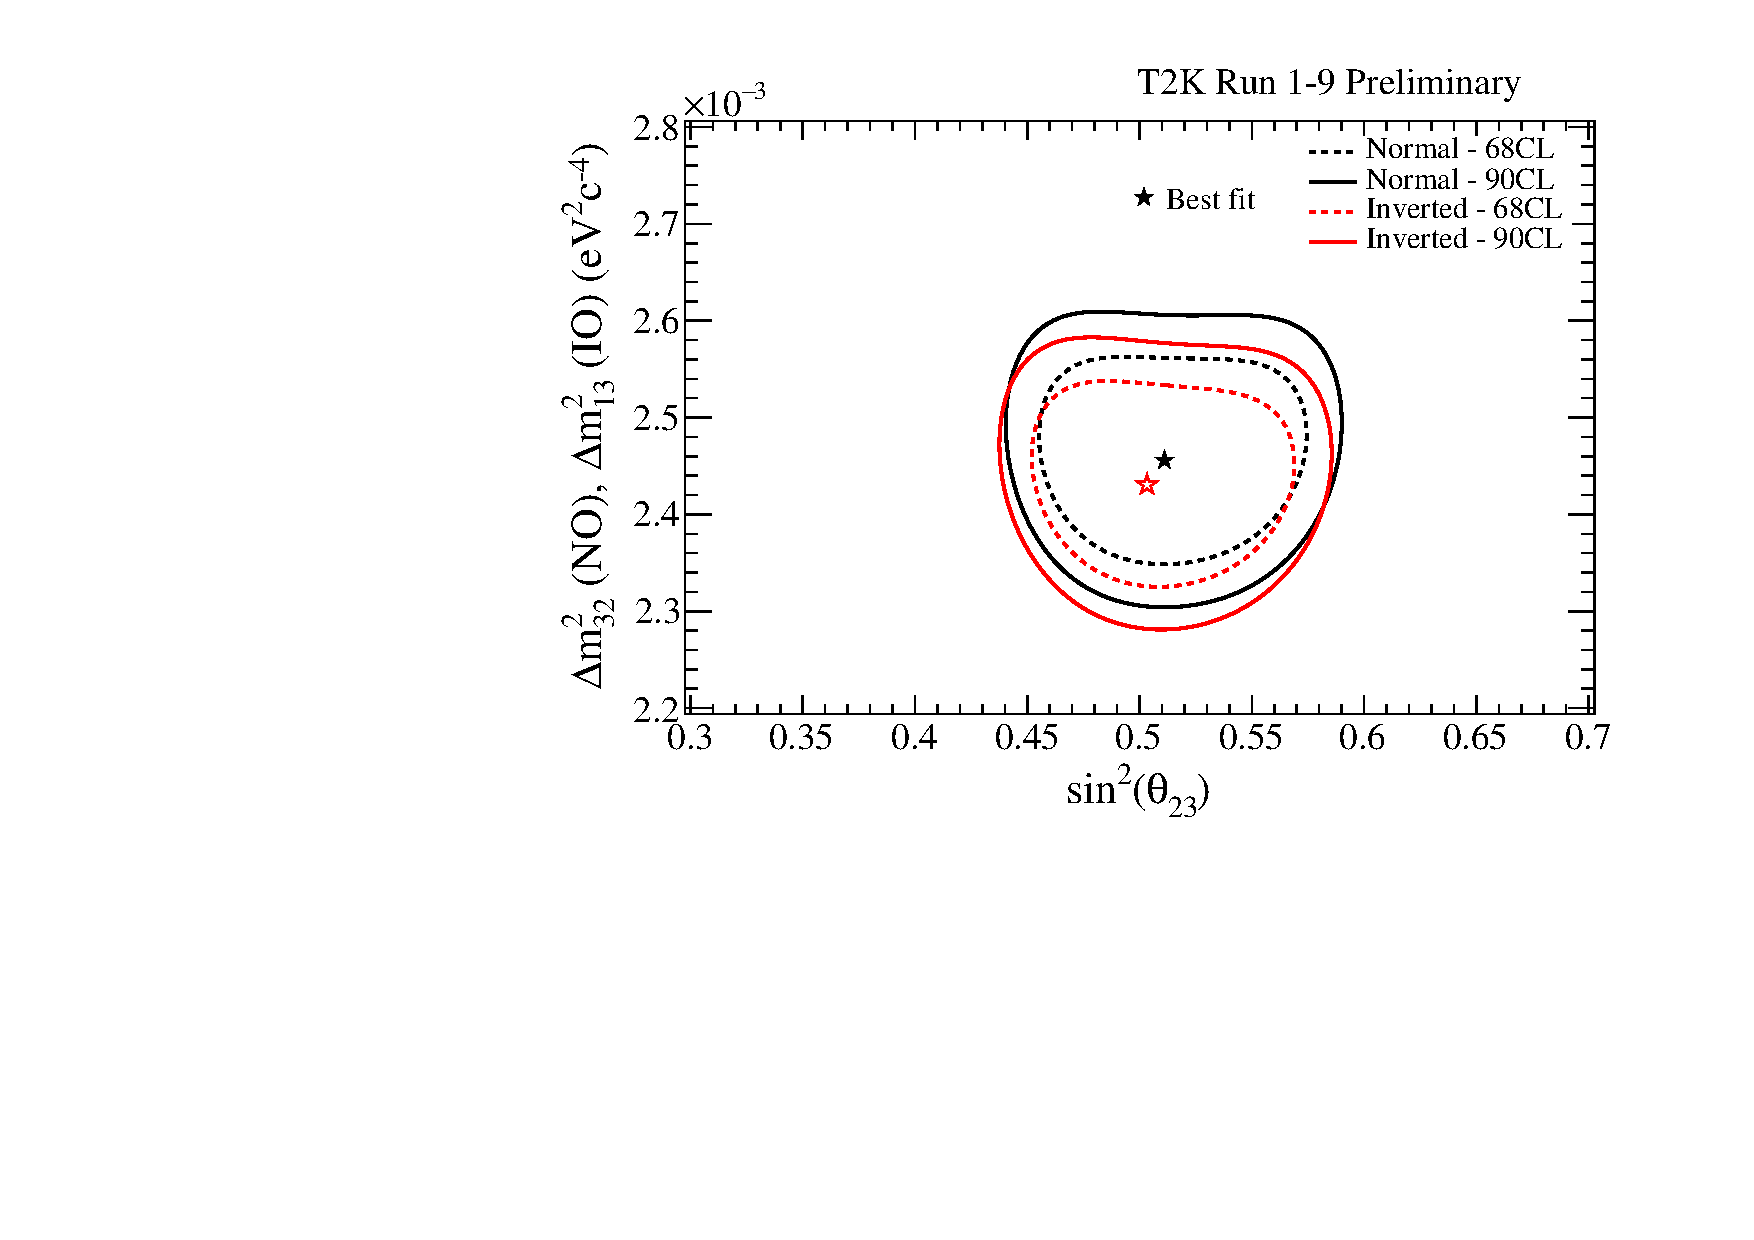
\includegraphics[width=0.9\textwidth]{images/data/mixing23_dmsq23_data_t2k_global}
		\caption{\disappearance T2K only}
	\end{subfigure}
	\caption {
		Contours at 68\% and 90\% CL for \disappearance with and without reactor constraint. Normal and inverted hierarchy contours are independent. All 5 samples were used to produce these fits.
	}
	\label{fig:ssqth23_vs_dmsq23_data}
\end{figure*}

\subsection{Results for \deltacp}

The result for \deltacp with reactor constraint and T2K only is shown in fig.~\ref{fig:dcp_data}.

\begin{figure*}[htb]
	\center
	\begin{subfigure}[b]{0.49\textwidth}
		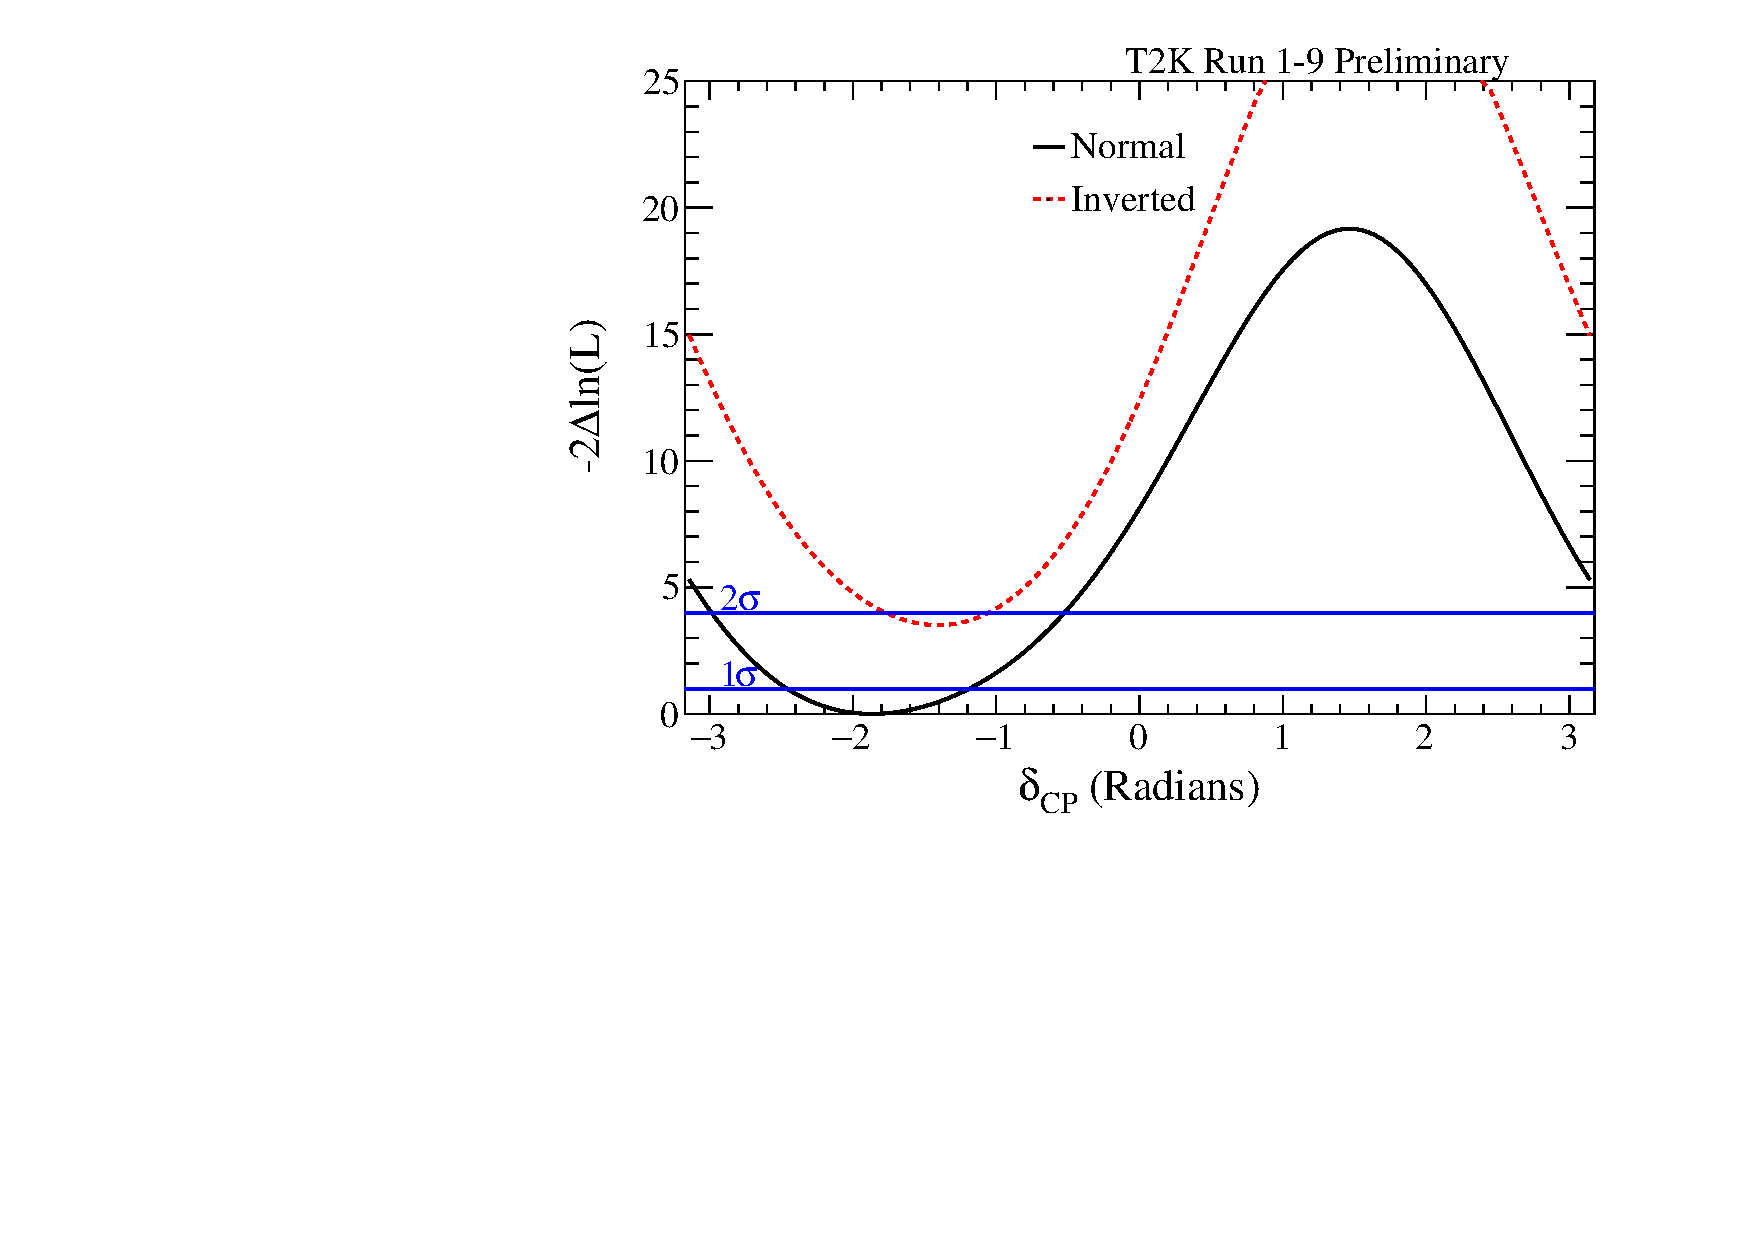
\includegraphics[width=0.9\textwidth]{images/data/deltacp_data_reactor_global}
		\caption{\deltacp with reactor constraint}
	\end{subfigure}
	\begin{subfigure}[b]{0.49\textwidth}
		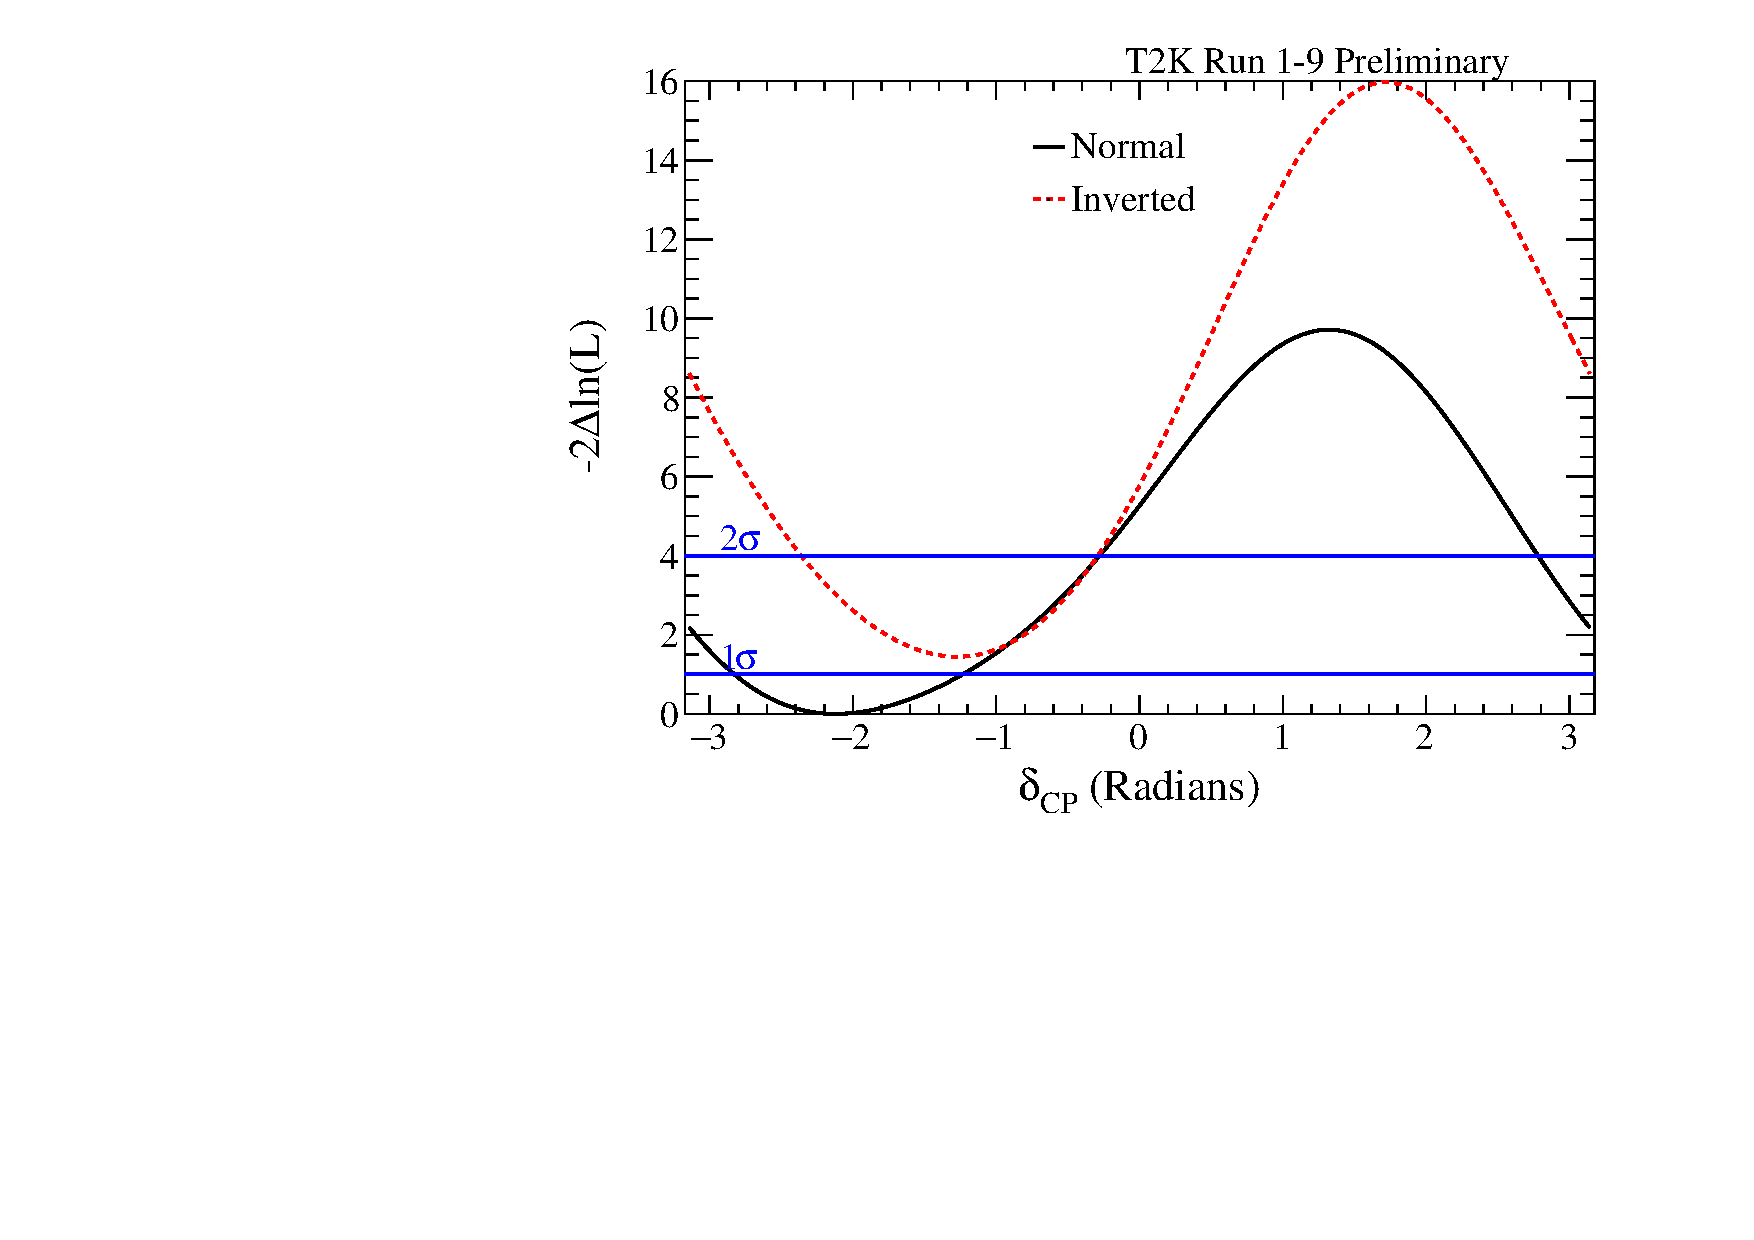
\includegraphics[width=0.9\textwidth]{images/data/deltacp_data_t2k_global}
		\caption{\deltacp T2K only}
	\end{subfigure}
	\caption {
		The expected $\Delta\chi^2$ distribution as a function of \deltacp with and without reactor constraint. The mass hierarchy is minimized, with normal and inverted hierarchy $\Delta\chi^2$ distributions shifted to the same global best-fit $\chi^2$ value, which is taken to be the minimum between normal and inverted hierarchy. All 5 samples were used to produce these fits.
	}
	\label{fig:dcp_data}
\end{figure*}

\clearpage

\subsection{Results for \ssqthonethree}

The result for \ssqthonethree (without reactor constraint) is shown in fig.~\ref{fig:th13_data}.

\begin{figure*}[htb]
	\center
	\begin{subfigure}[b]{0.49\textwidth}
		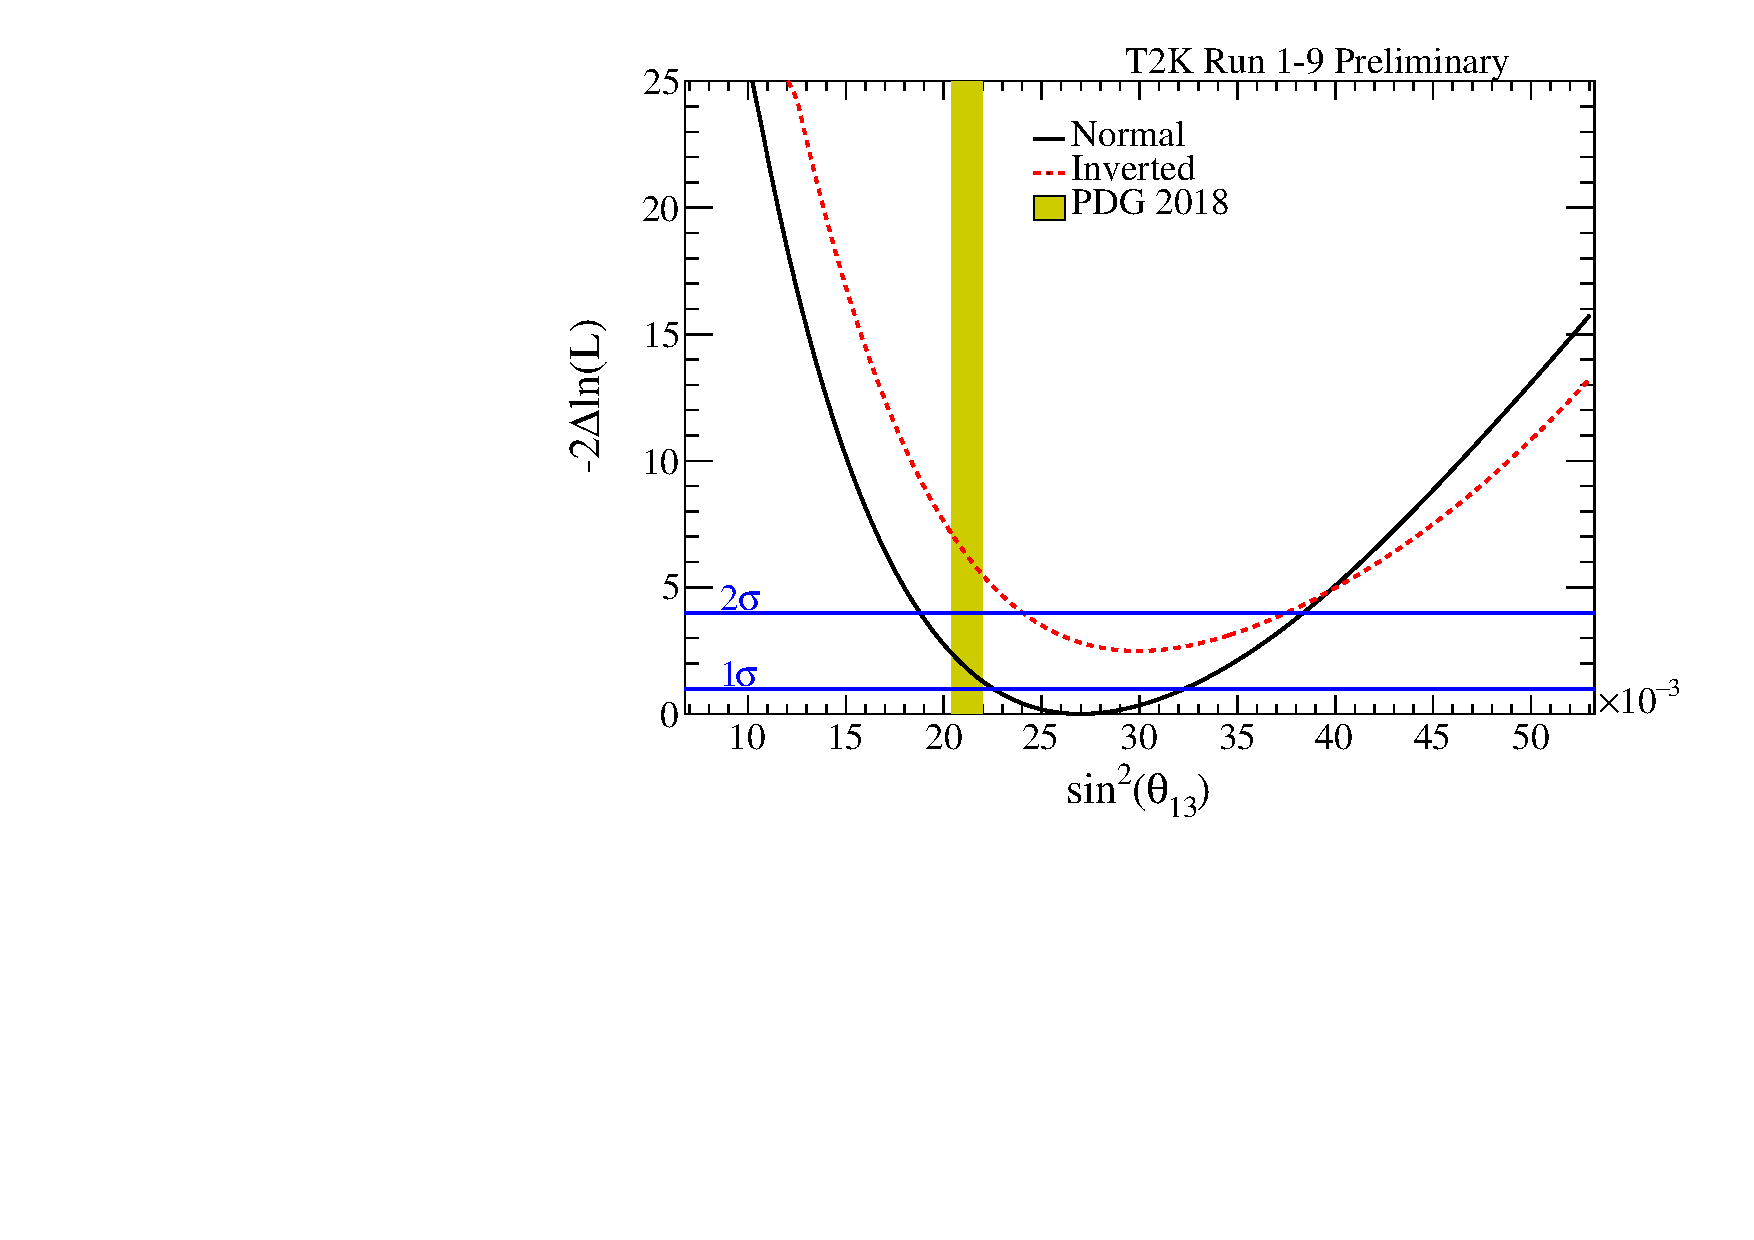
\includegraphics[width=0.9\textwidth]{images/data/mixing13_data_t2k_global}
		\caption{\ssqthonethree T2K only}
	\end{subfigure}
	\caption {
		The expected $\Delta\chi^2$ distribution as a function of \ssqthonethree without reactor constraint. The mass hierarchy is minimized, with normal and inverted hierarchy $\Delta\chi^2$ distributions shifted to the same global best-fit $\chi^2$ value, which is taken to be the minimum between normal and inverted hierarchy. All 5 samples were used to produce these fits.
	}
	\label{fig:th13_data}
\end{figure*}

\subsection{Results for \ssqthtwothree}

The result for \ssqthtwothree with reactor constraint and T2K only is shown in fig.~\ref{fig:th23_data}.

\begin{figure*}[htb]
	\center
	\begin{subfigure}[b]{0.49\textwidth}
		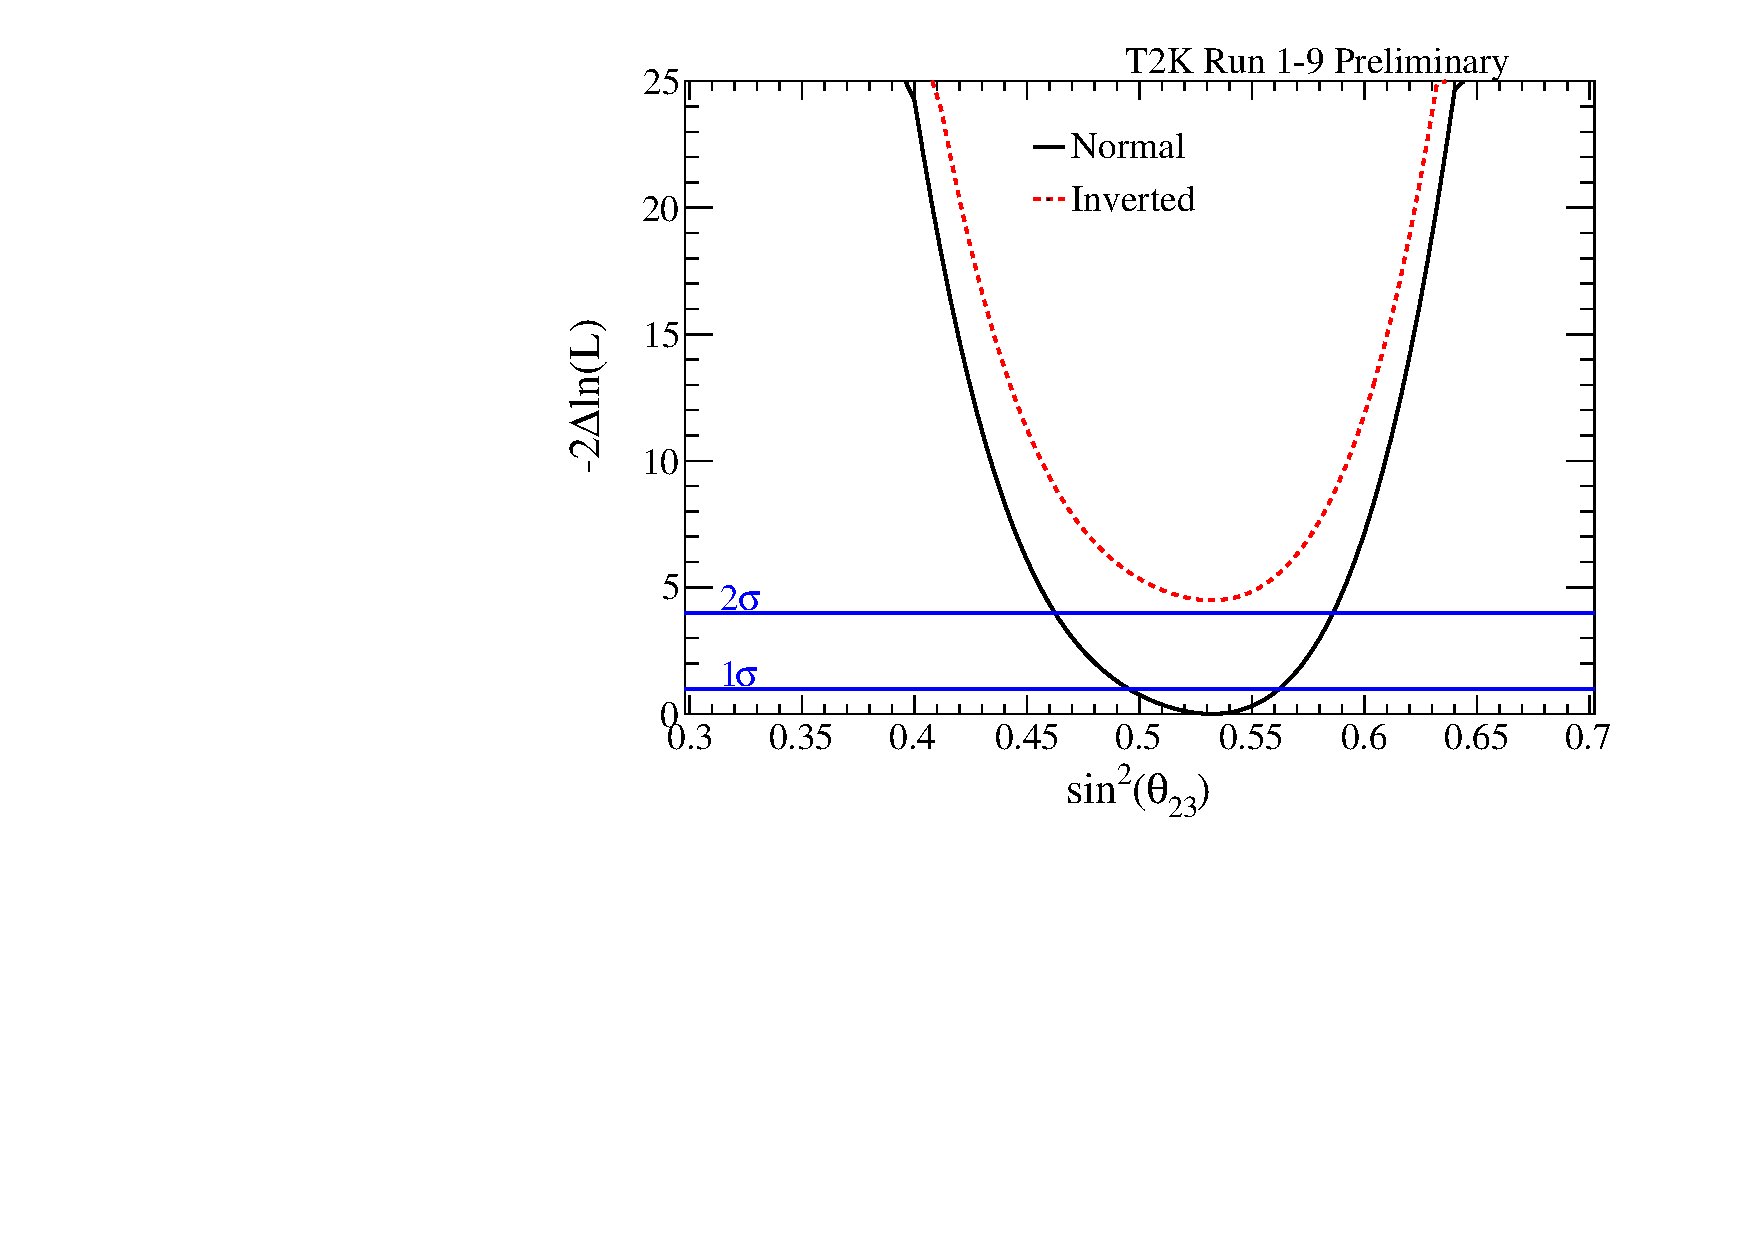
\includegraphics[width=0.9\textwidth]{images/data/mixing23_data_reactor_global}
		\caption{\ssqthtwothree with reactor constraint}
	\end{subfigure}
	\begin{subfigure}[b]{0.49\textwidth}
		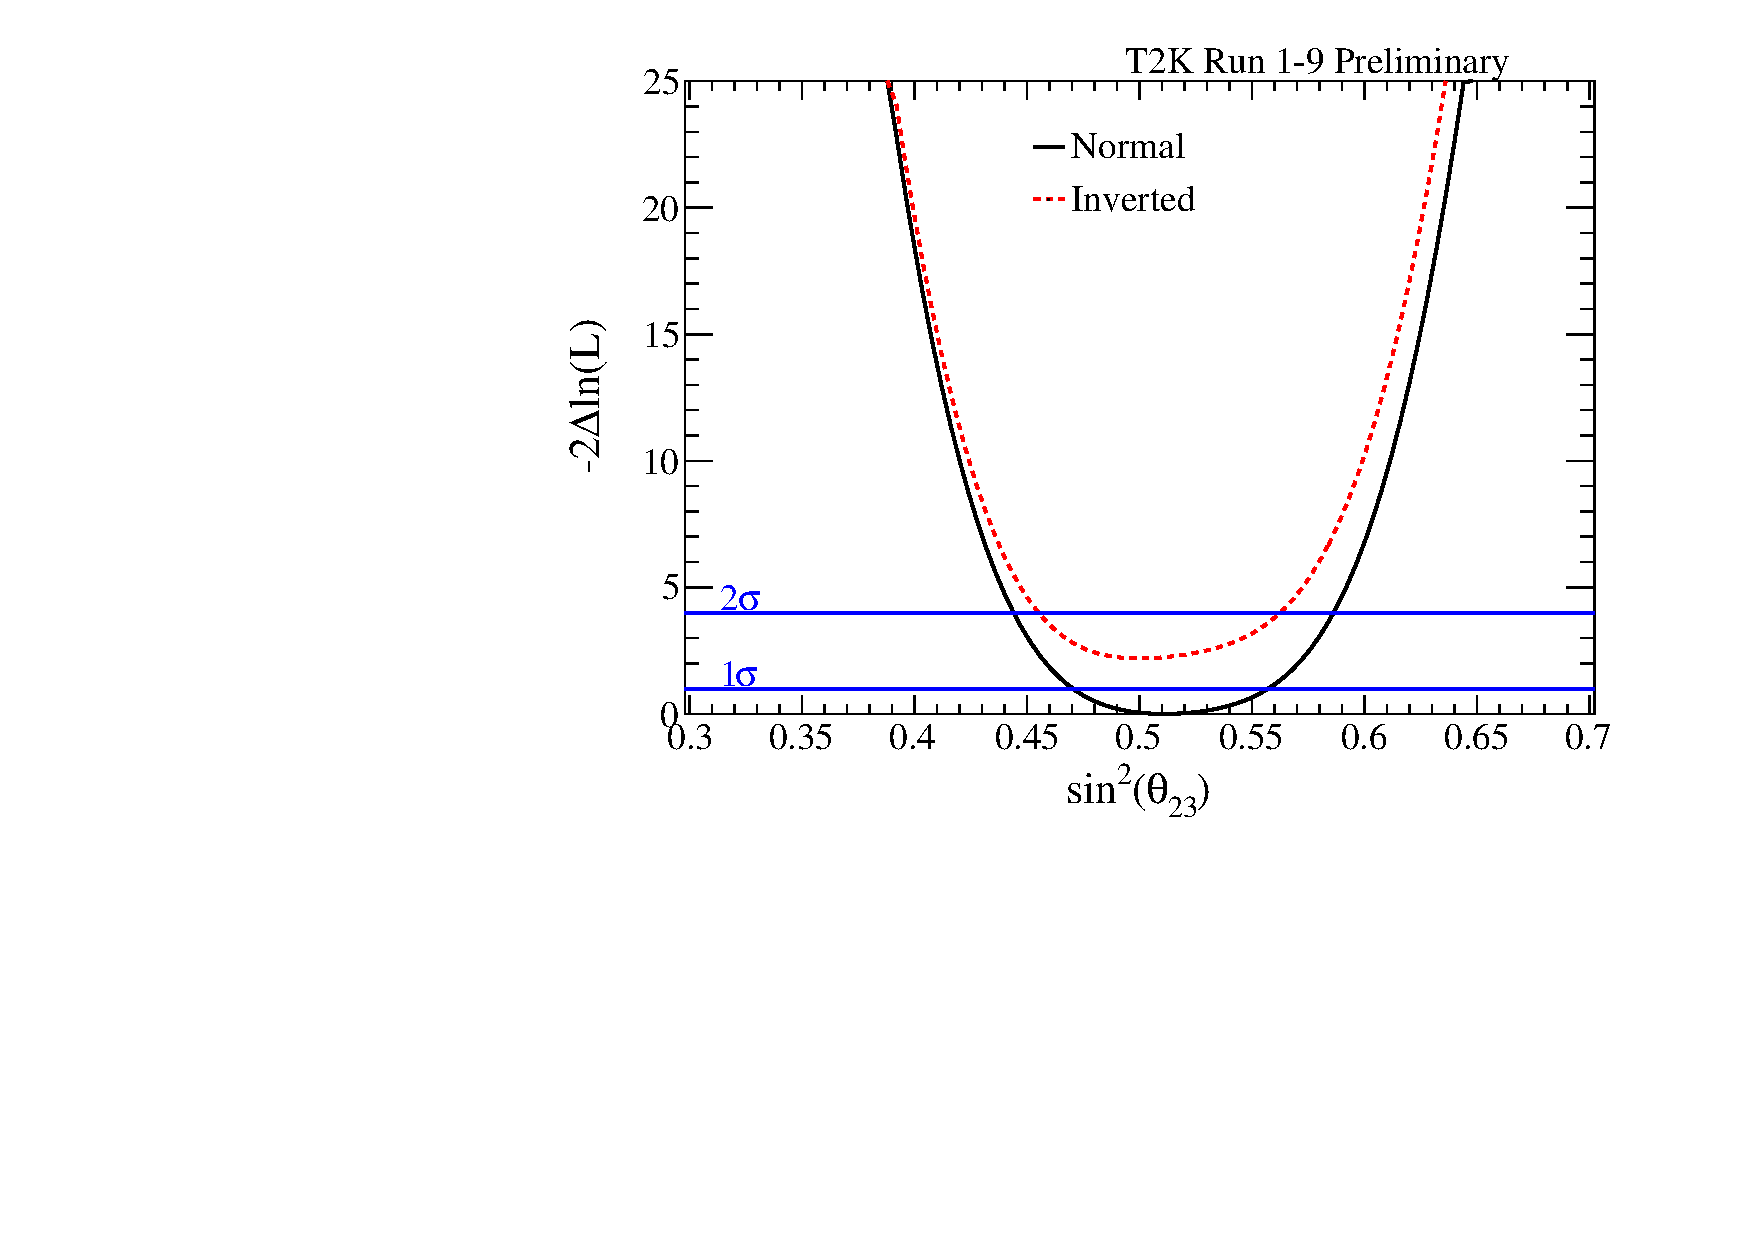
\includegraphics[width=0.9\textwidth]{images/data/mixing23_data_t2k_global}
		\caption{\ssqthtwothree T2K only}
	\end{subfigure}
	\caption {
		The expected $\Delta\chi^2$ distribution as a function of \ssqthtwothree with and without reactor constraint. The mass hierarchy is minimized, with normal and inverted hierarchy $\Delta\chi^2$ distributions shifted to the same global best-fit $\chi^2$ value, which is taken to be the minimum between normal and inverted hierarchy. All 5 samples were used to produce these fits.
	}
	\label{fig:th23_data}
\end{figure*}

\clearpage

\subsection{Results for \dmsq}

The result for \dmsq with reactor constraint and T2K only is shown in fig.~\ref{fig:dmsq23_data}.

\begin{figure*}[htb]
	\center
	\begin{subfigure}[b]{0.49\textwidth}
		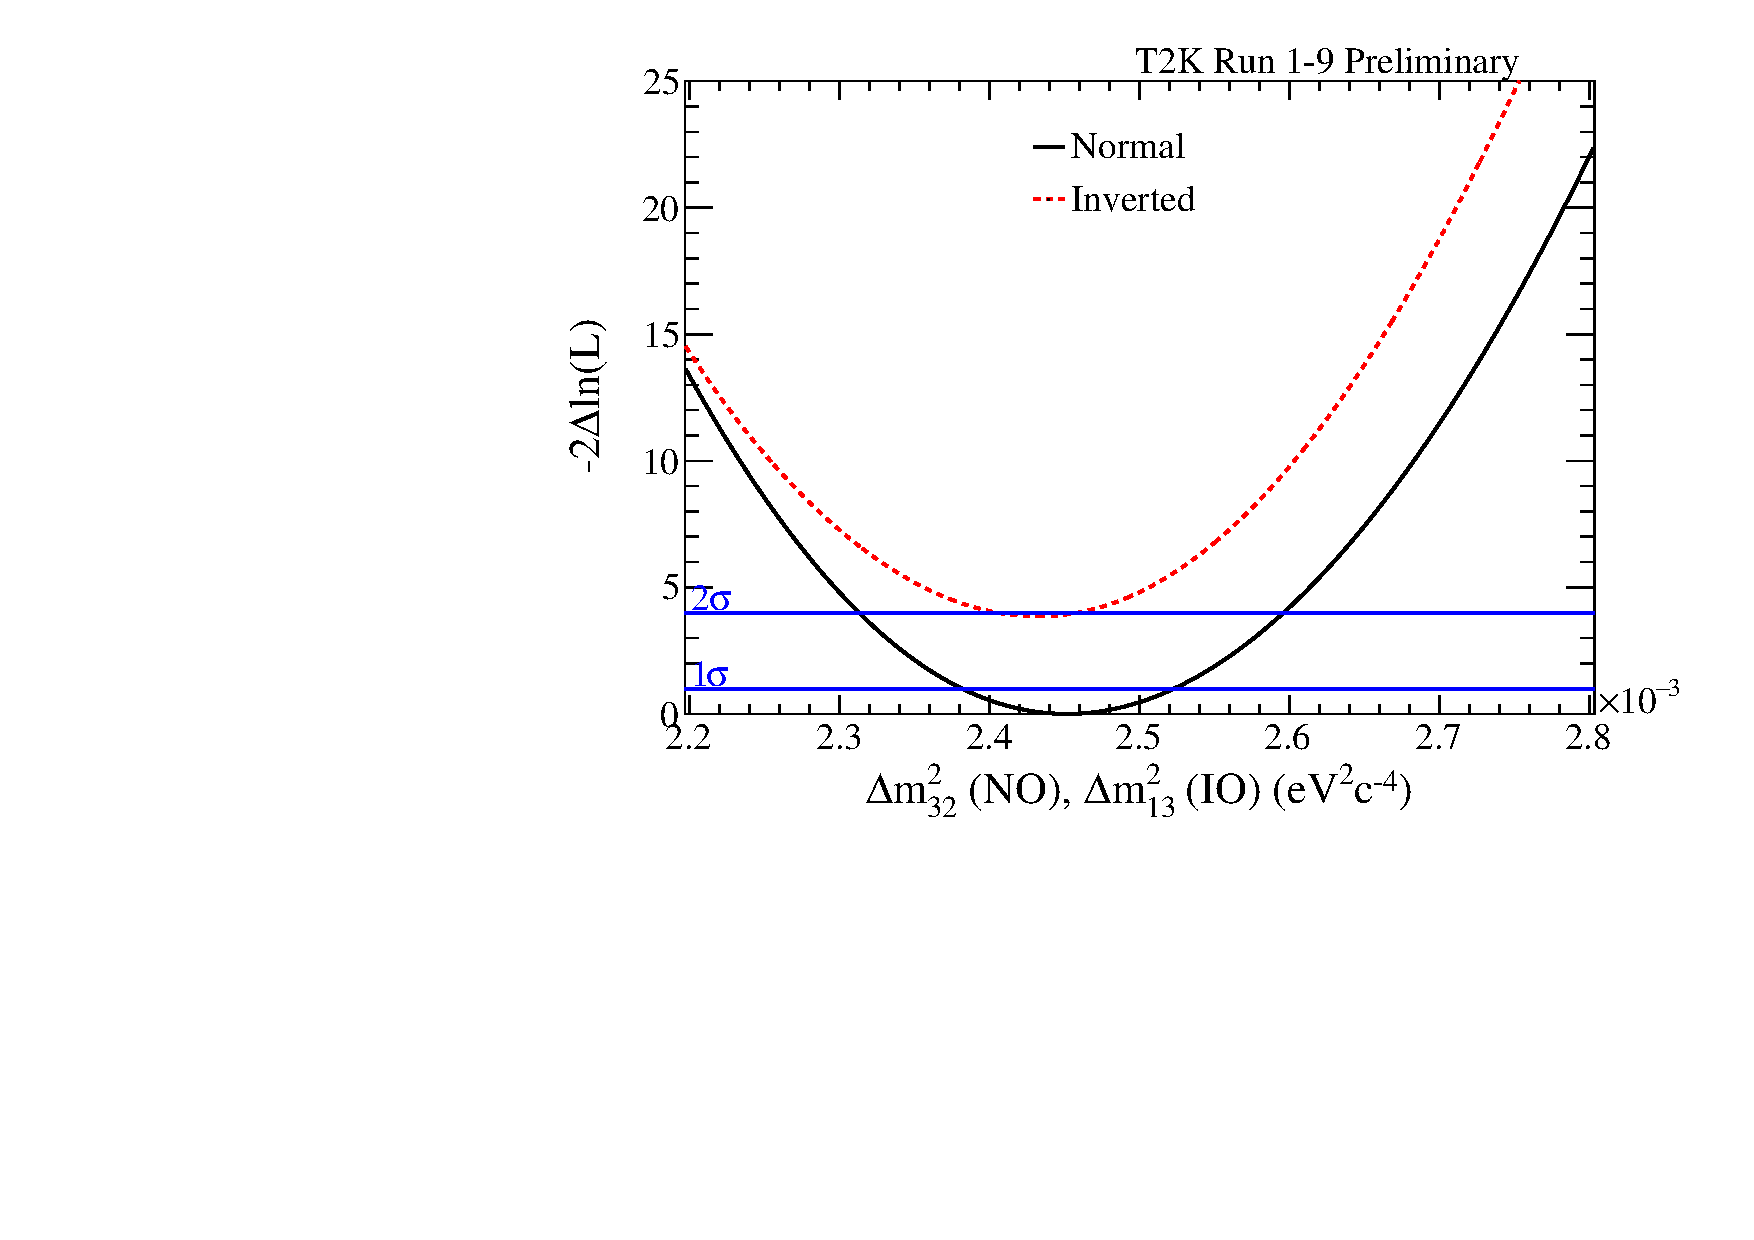
\includegraphics[width=0.9\textwidth]{images/data/dmsq23_data_reactor_global}
		\caption{\dmsq with reactor constraint}
	\end{subfigure}
	\begin{subfigure}[b]{0.49\textwidth}
		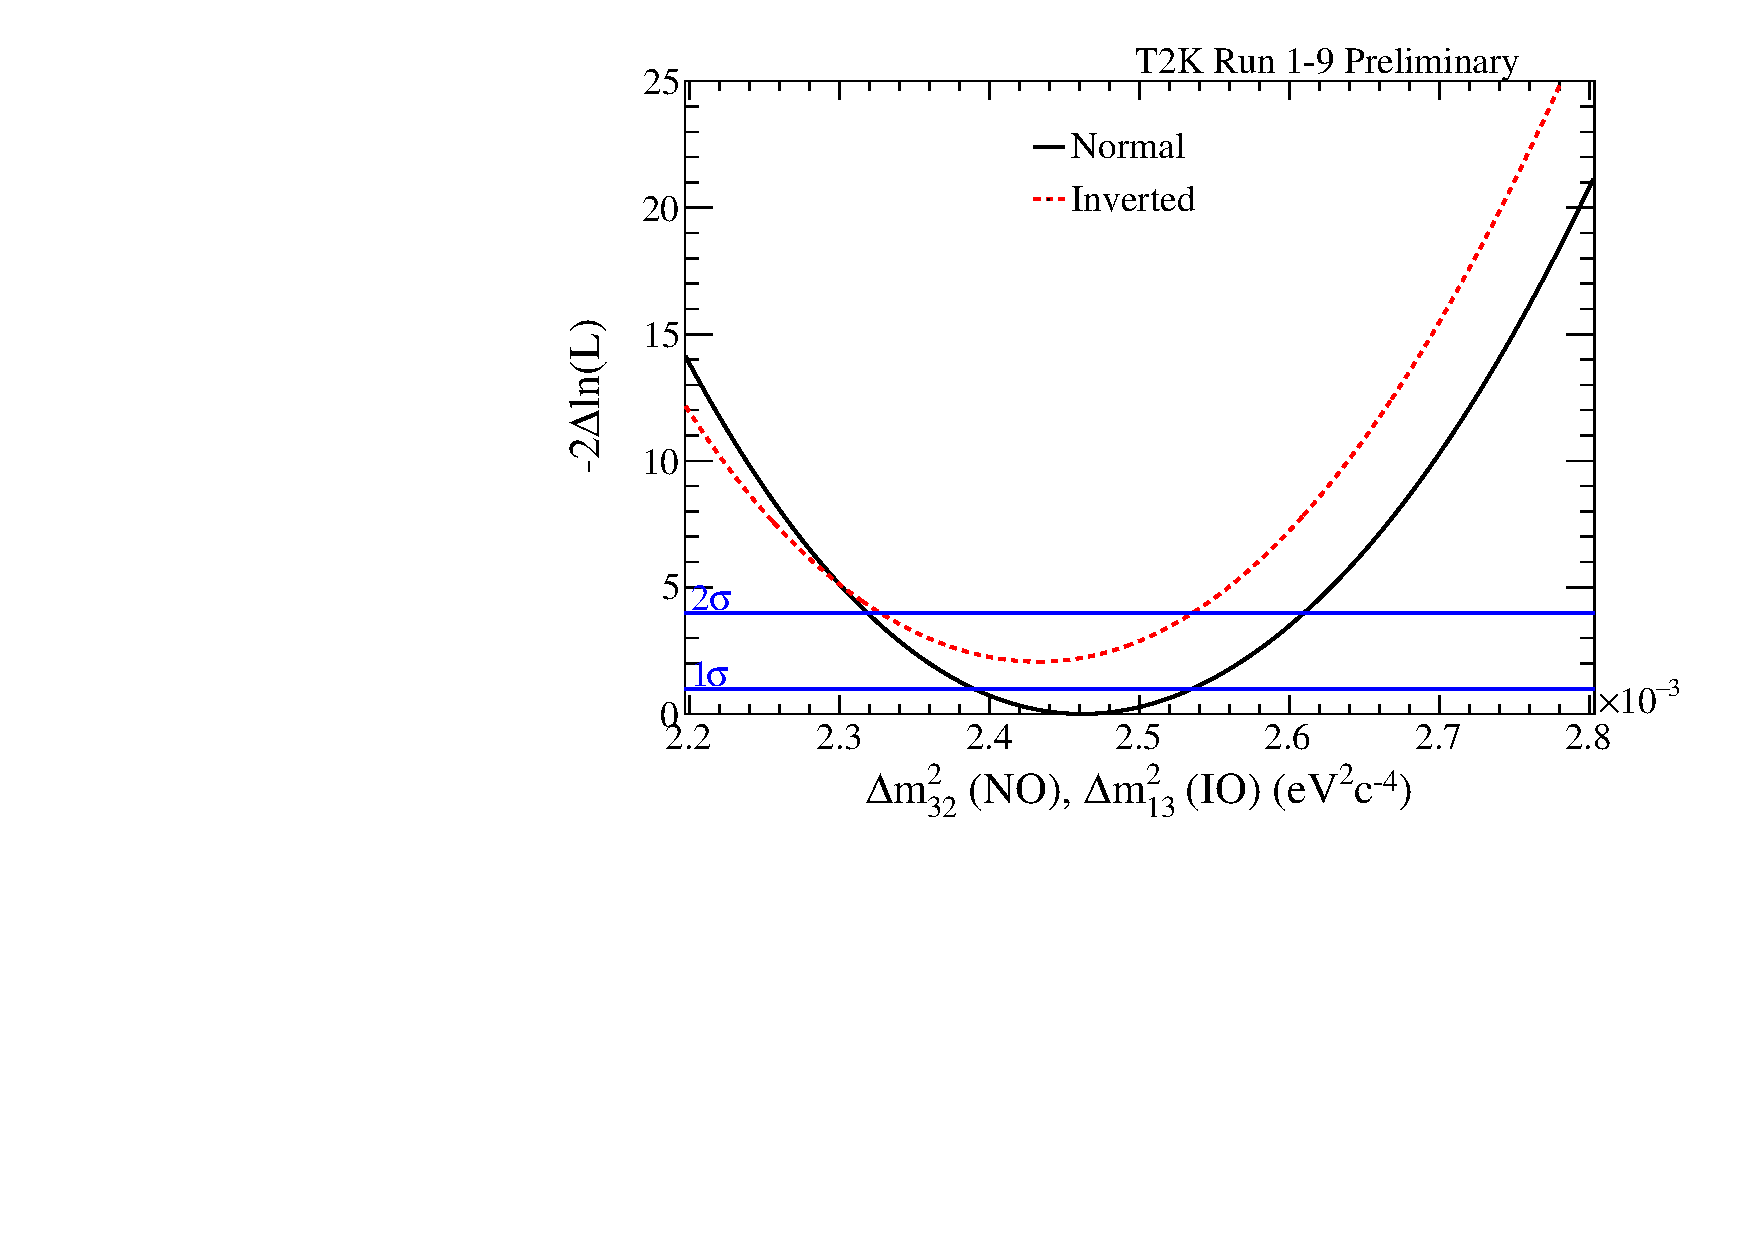
\includegraphics[width=0.9\textwidth]{images/data/dmsq23_data_t2k_global}
		\caption{\dmsq T2K only}
	\end{subfigure}
	\caption {
		The expected $\Delta\chi^2$ distribution as a function of \dmsqtwothree with and without reactor constraint. The mass hierarchy is minimized, with normal and inverted hierarchy $\Delta\chi^2$ distributions shifted to the same global best-fit $\chi^2$ value, which is taken to be the minimum between normal and inverted hierarchy. All 5 samples were used to produce these fits.
	}
	\label{fig:dmsq23_data}
\end{figure*}

\FloatBarrier

\subsection {Feldman-Cousins simultaneous fit of \deltacp and mass hierarchy}
\label{sec:fc_significance}

This section presents the results of the Feldman-Cousins fit of \deltacp and mass hierarchy. The method is the same as that used in \cite{OurRun18JointAnalysis3Flavour}, in particular throws of oscillation parameters are made according to PDG 2018 best-fit values and errors for \ssqthonethree, \ssqthonetwo and \dmsqonetwo, whilst, \ssqthtwothree and \dmsq are thrown from the likelihood surface produced by an Asimov fit. To produce this likelihood surface, an Asimov data set is defined using the PDG 2018 best fits for \ssqthonetwo and \dmsqonetwo, and the unsmeared best-fit values from the 2D reactor data fits in their respective hierarchies. \deltacp is then fixed at one of 9 evenly specified values on the range $\left[-\pi,\pi\right]$. To accommodate the inclusion of $3\sigma$ intervals the number of Feldman-Cousins toys has been increased from 10K to 20K.

\subsubsection{Input oscillation parameters}
\label{sec:fc_significance:inputs}

The distributions of oscillation parameters are shown in \cref{fig:fc_input_dist}.

\begin{figure*}[htb]
	\center
	\begin{subfigure}[b]{0.49\textwidth}
		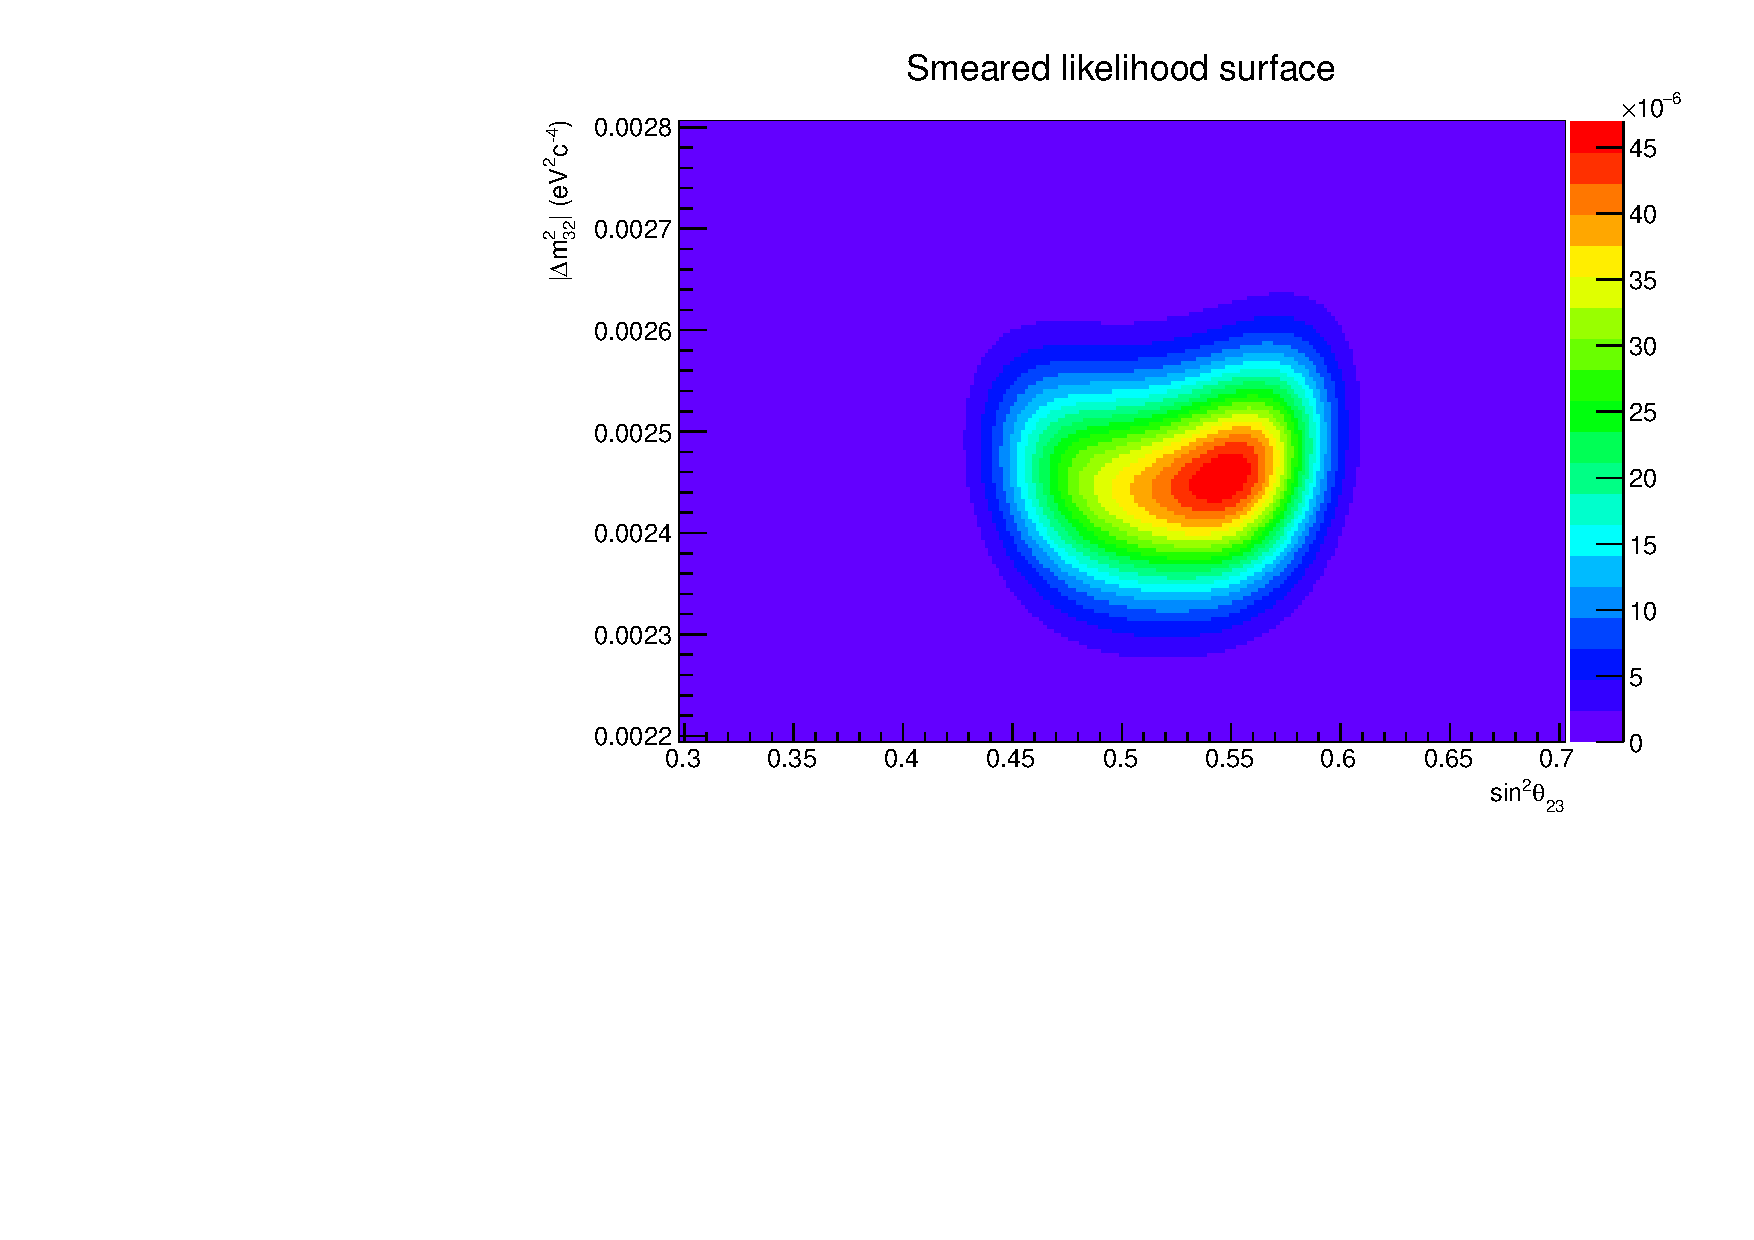
\includegraphics[width=0.9\textwidth]{images/fc/inputs/smear_reactor_normal}
		\caption{Normal hierarchy}
	\end{subfigure}
	\begin{subfigure}[b]{0.49\textwidth}
		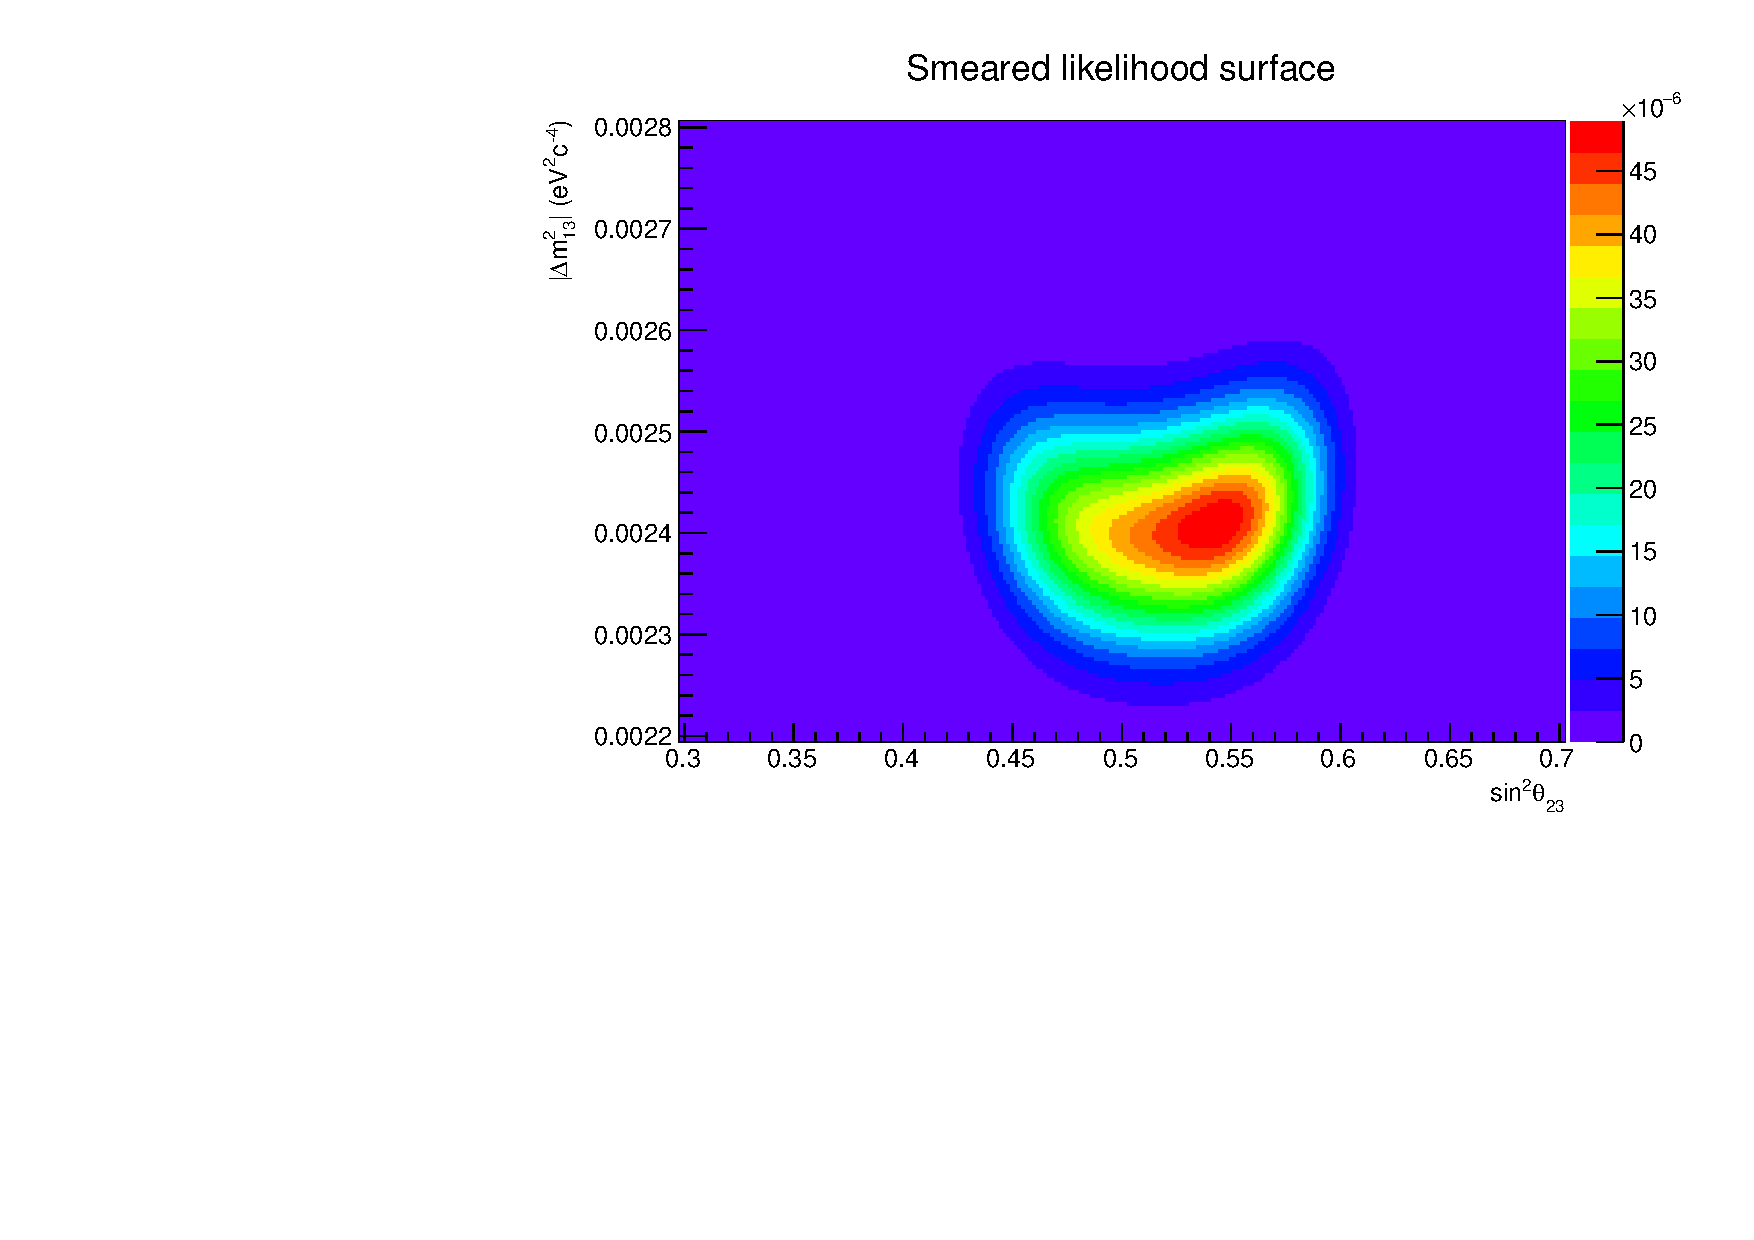
\includegraphics[width=0.9\textwidth]{images/fc/inputs/smear_reactor_inverted}
		\caption{Inverted hierarchy}
	\end{subfigure}
	\begin{subfigure}[b]{0.49\textwidth}
		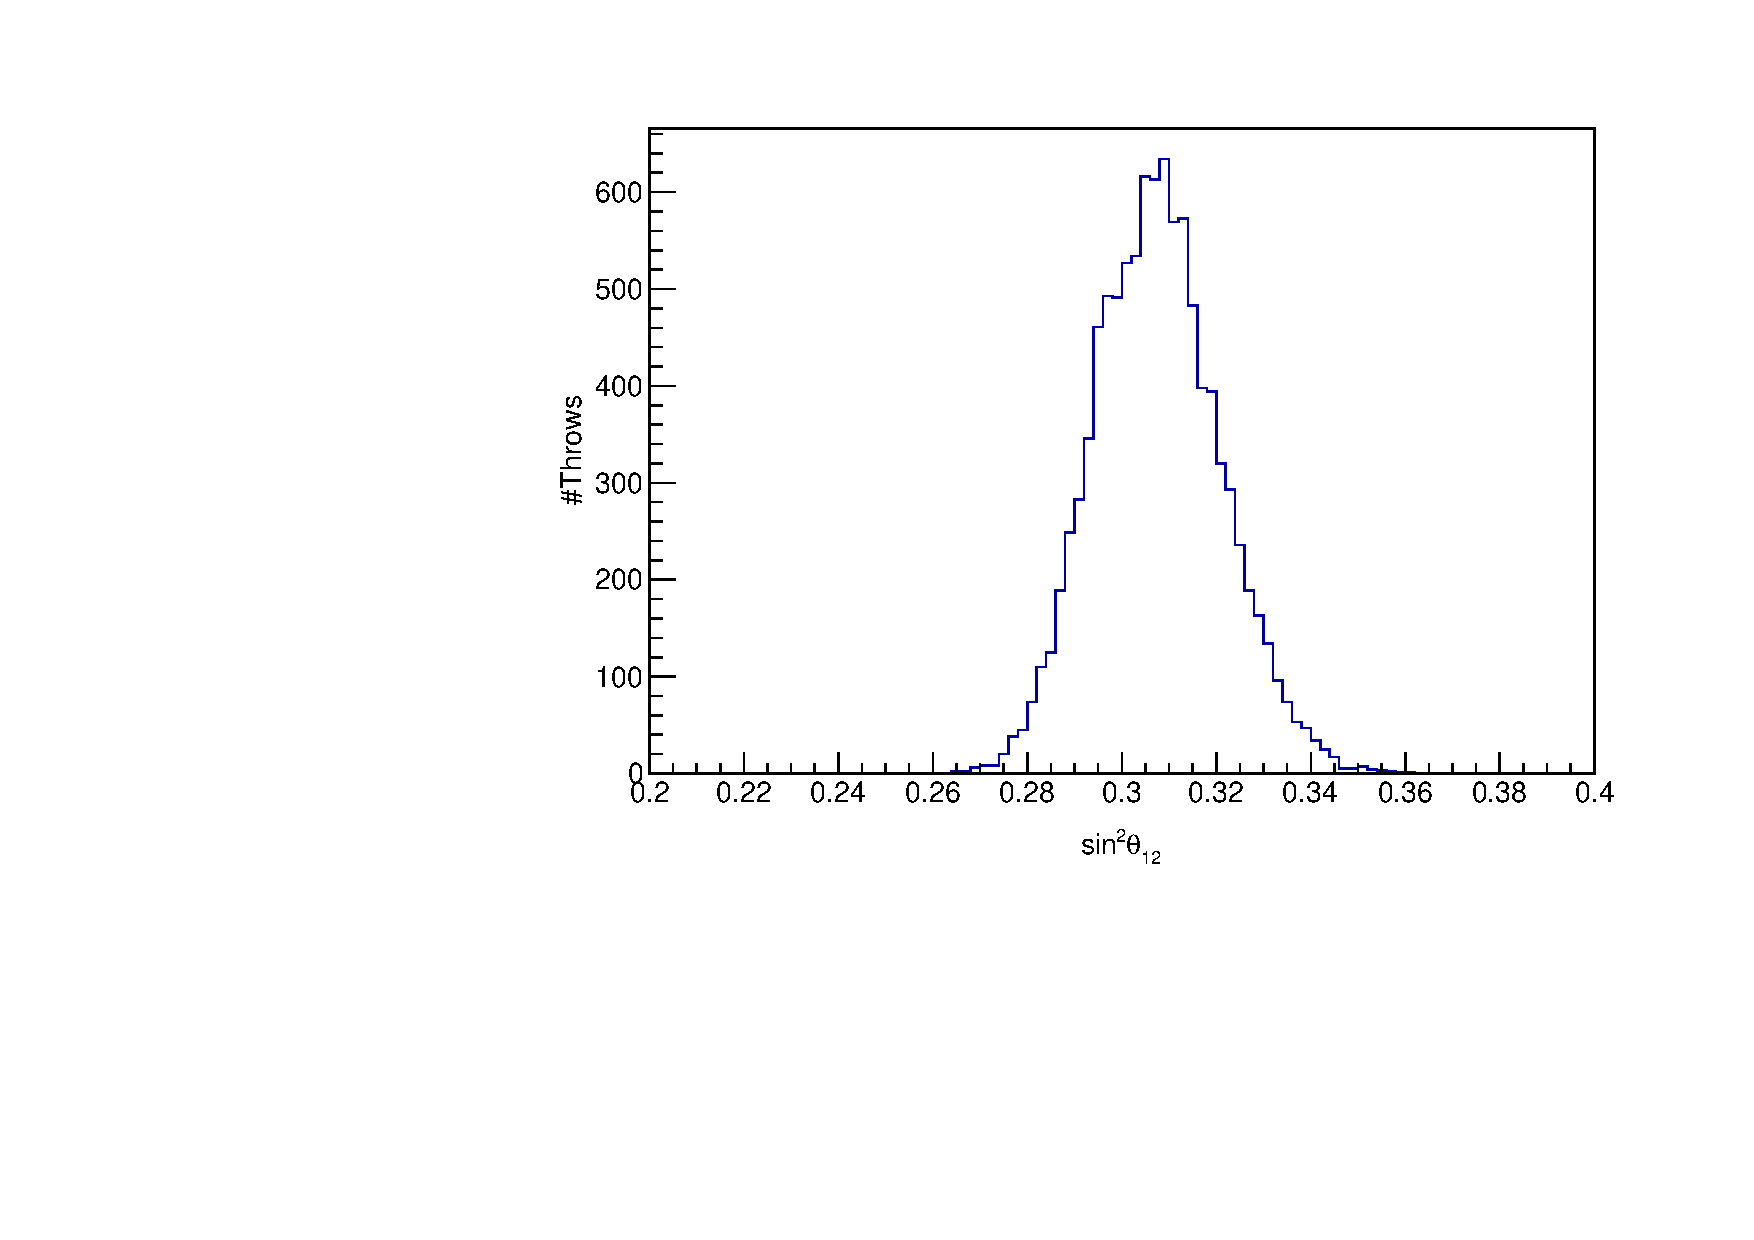
\includegraphics[page=1, width=0.9\textwidth]{images/fc/inputs/fc_inputs}
		\caption{\ssqthonetwo}
	\end{subfigure}
	\begin{subfigure}[b]{0.49\textwidth}
		\includegraphics[page=2, width=0.9\textwidth]{images/fc/inputs/fc_inputs}
		\caption{\dmsqonetwo}
	\end{subfigure}
	\begin{subfigure}[b]{0.49\textwidth}
		\includegraphics[page=3, width=0.9\textwidth]{images/fc/inputs/fc_inputs}
		\caption{\ssqthonethree}
	\end{subfigure}
	\caption {
		Distribution of oscillation parameter throws for Feldman-Cousins fits.
	}
	\label{fig:fc_input_dist}
\end{figure*}

\subsubsection{Feldman-Cousins critical values and confidence intervals}
\label{sec:fc_significance:intervals}
In \cref{fig:fc_interval} the confidence intervals obtained with the Feldman-Cousins method are shown for \deltacp and mass hierarchy with reactor constraint for the \RunPeriod data set. The critical values at $1\sigma$, 90\%, $2\sigma$ and $3\sigma$ CL are computed for both the mass hierarchies at the following true values of \deltacp; $-\pi$, $-3\pi/4$, $-\pi/2$, $-\pi/4$, 0, $+\pi/4$, $+\pi/2$, $+3\pi/4$, and $+\pi$. A small interval around $\delta_{CP} = -\pi/2$ is allowed in inverted hierarchy. Both $\delta_{CP} = 0$ and $\delta_{CP} = \pi$ are excluded at $2\sigma$. In \cref{tab:fc_interval} the $2\sigma$ CL intervals for \deltacp versus mass hierarchy, obtained with the Feldman-Cousins method, are shown. Comparison of critical values between VALOR and p-theta are provided in \cref{app:fc_compare}.

\begin{figure*}[htb]
	\center
	\begin{subfigure}[b]{0.6\textwidth}
		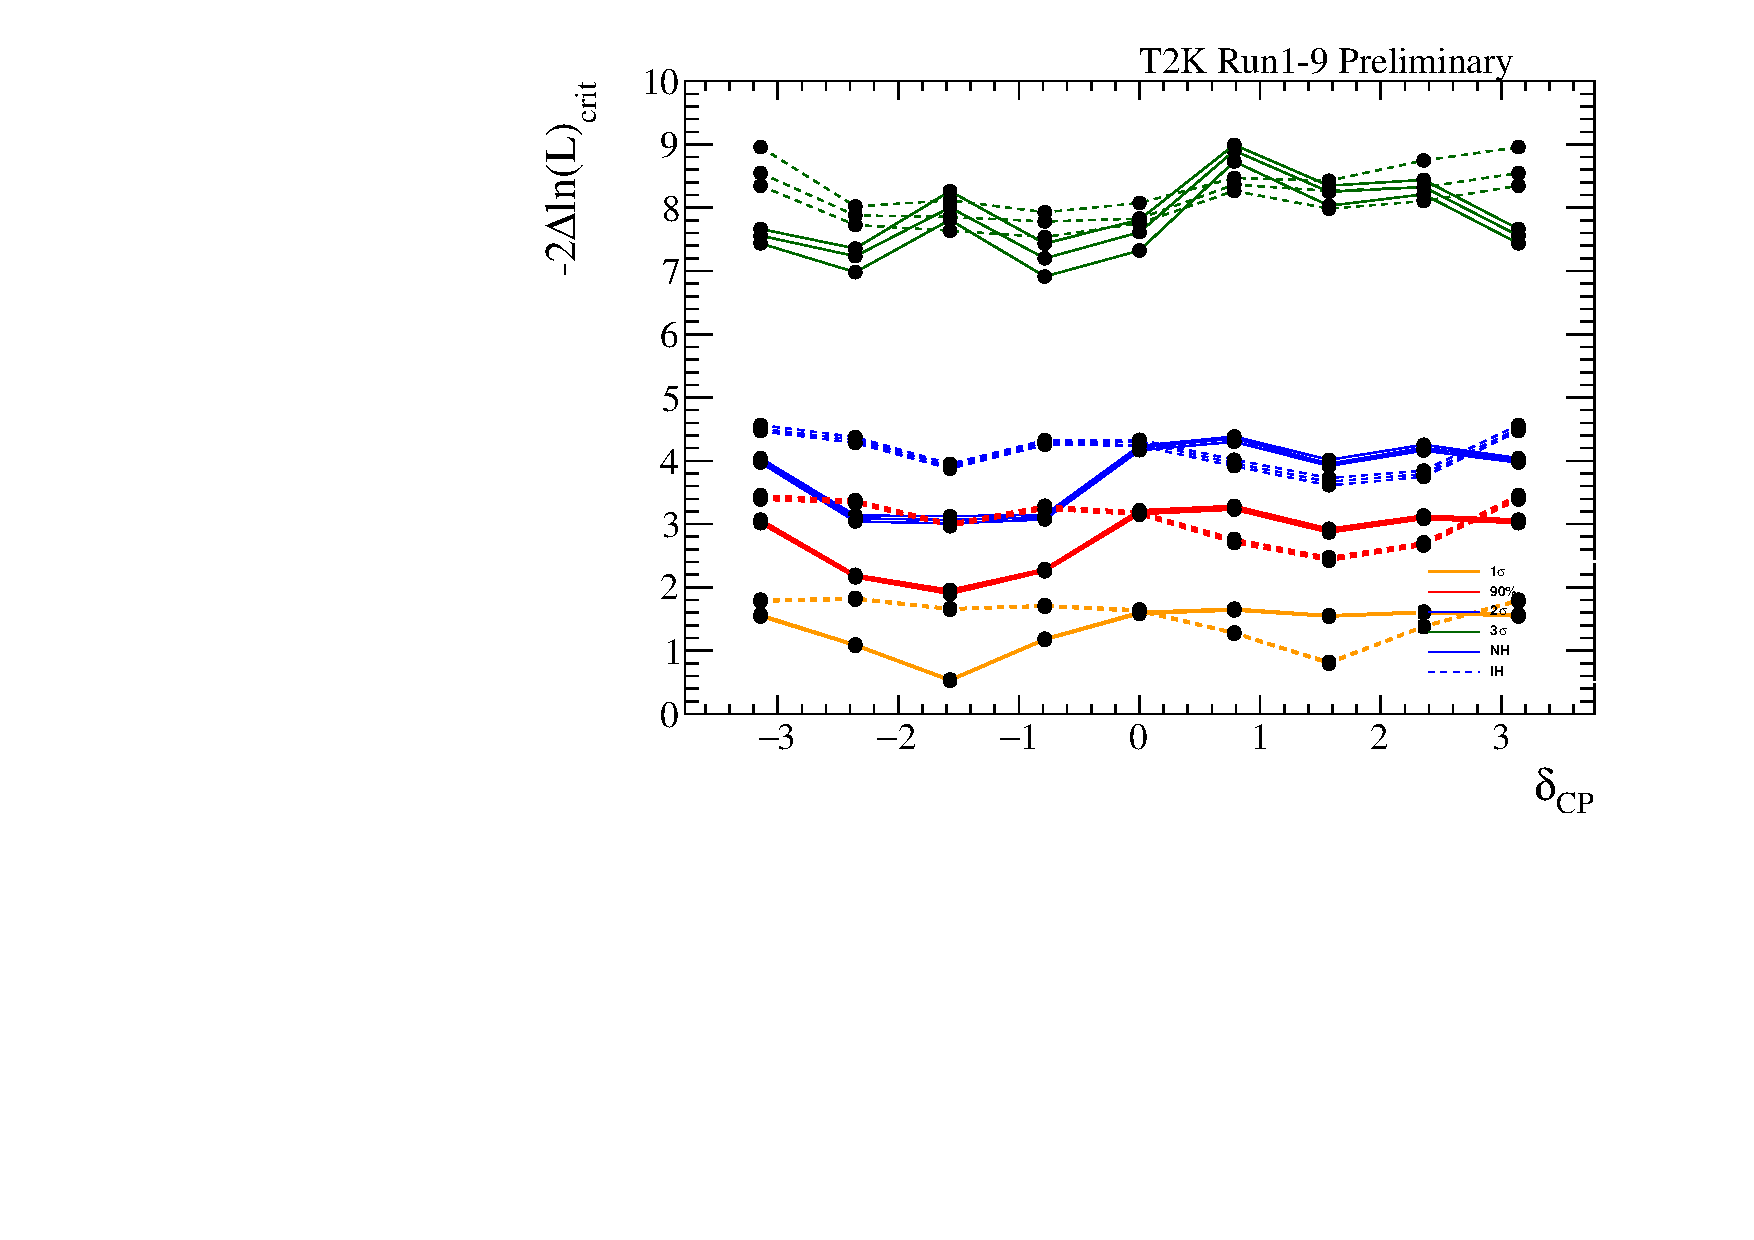
\includegraphics[width=0.9\textwidth]{images/fc/FC_critical_values}
		\caption{\label{fig:fc_critval}Critical $\Delta\chi^2$ values}
	\end{subfigure}
	\begin{subfigure}[b]{0.49\textwidth}
		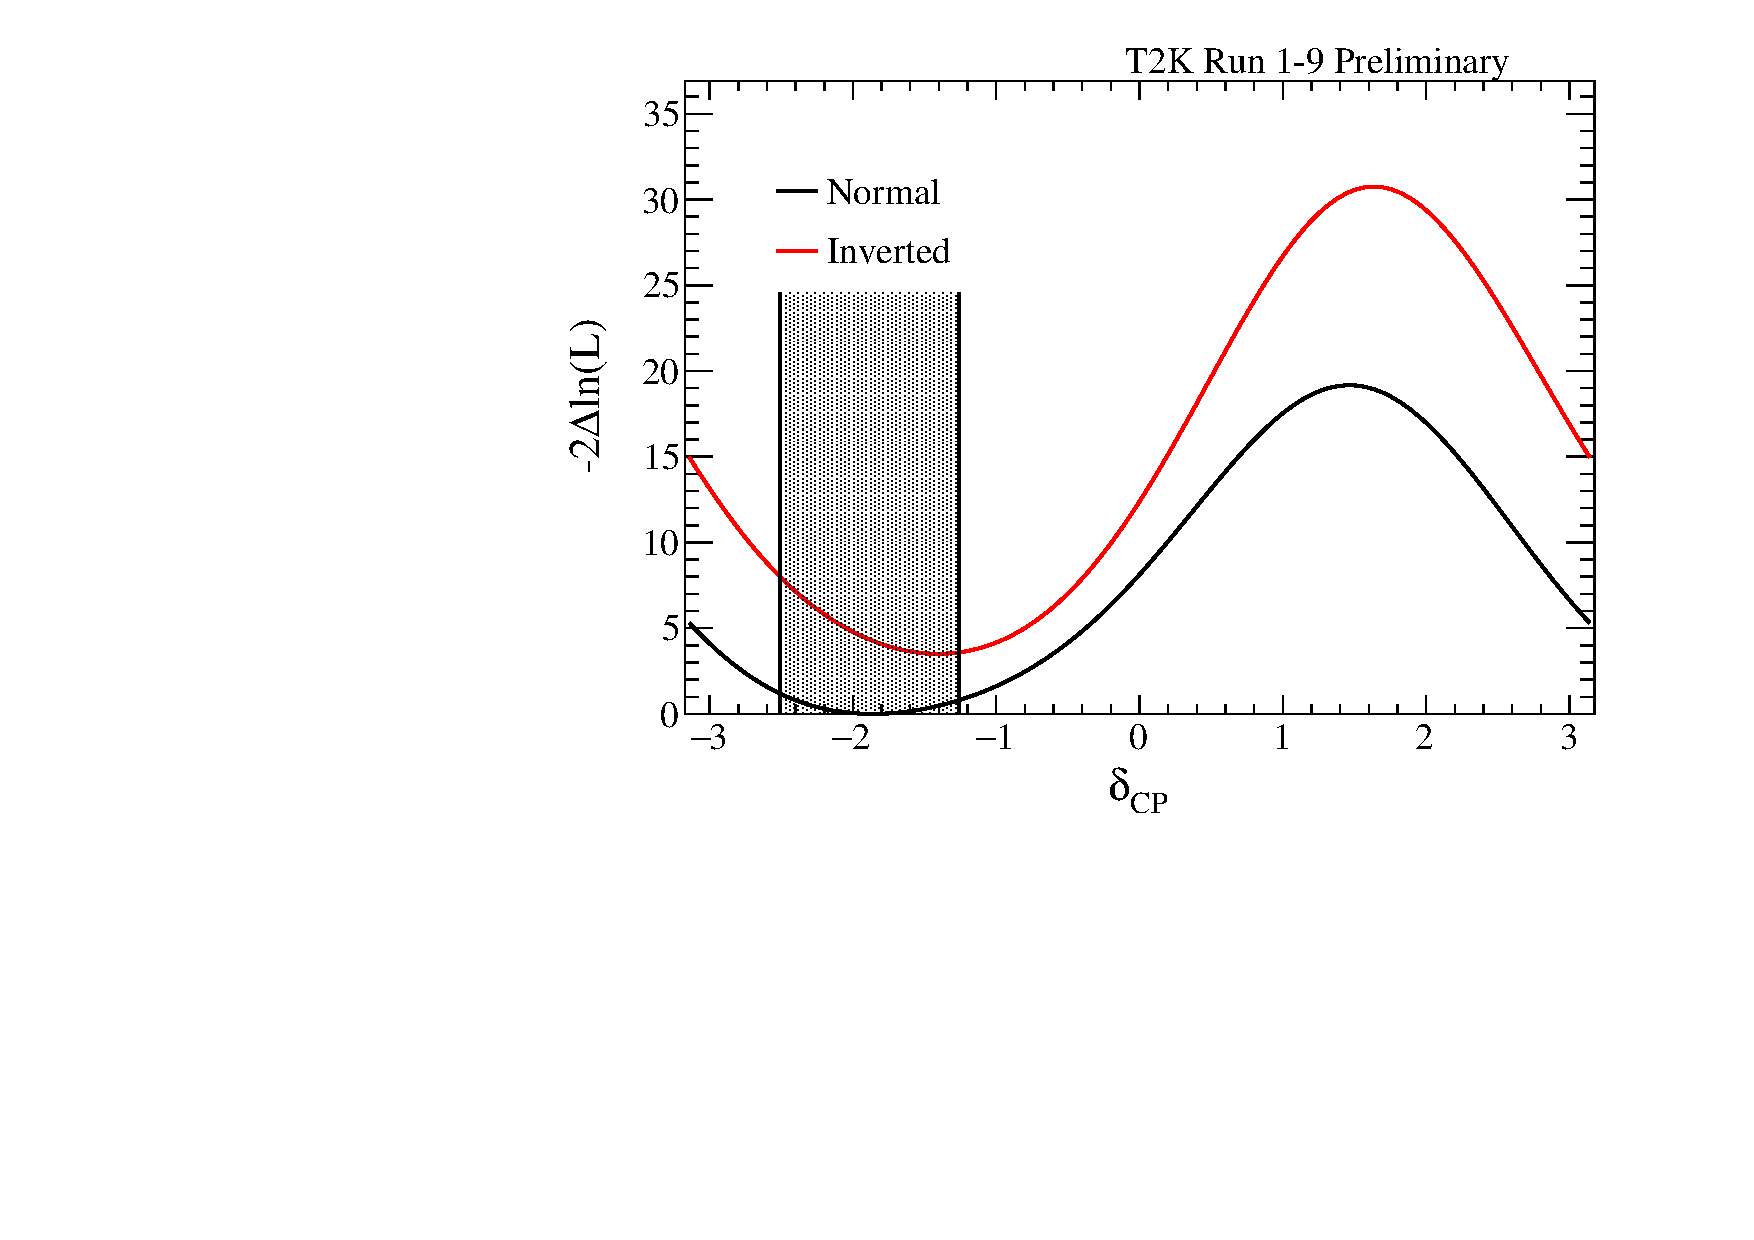
\includegraphics[width=0.9\textwidth]{images/fc/deltacp_mpi2_1sigma}
		\caption{$1\sigma$ CL exclusion region}
	\end{subfigure}
	\begin{subfigure}[b]{0.49\textwidth}
		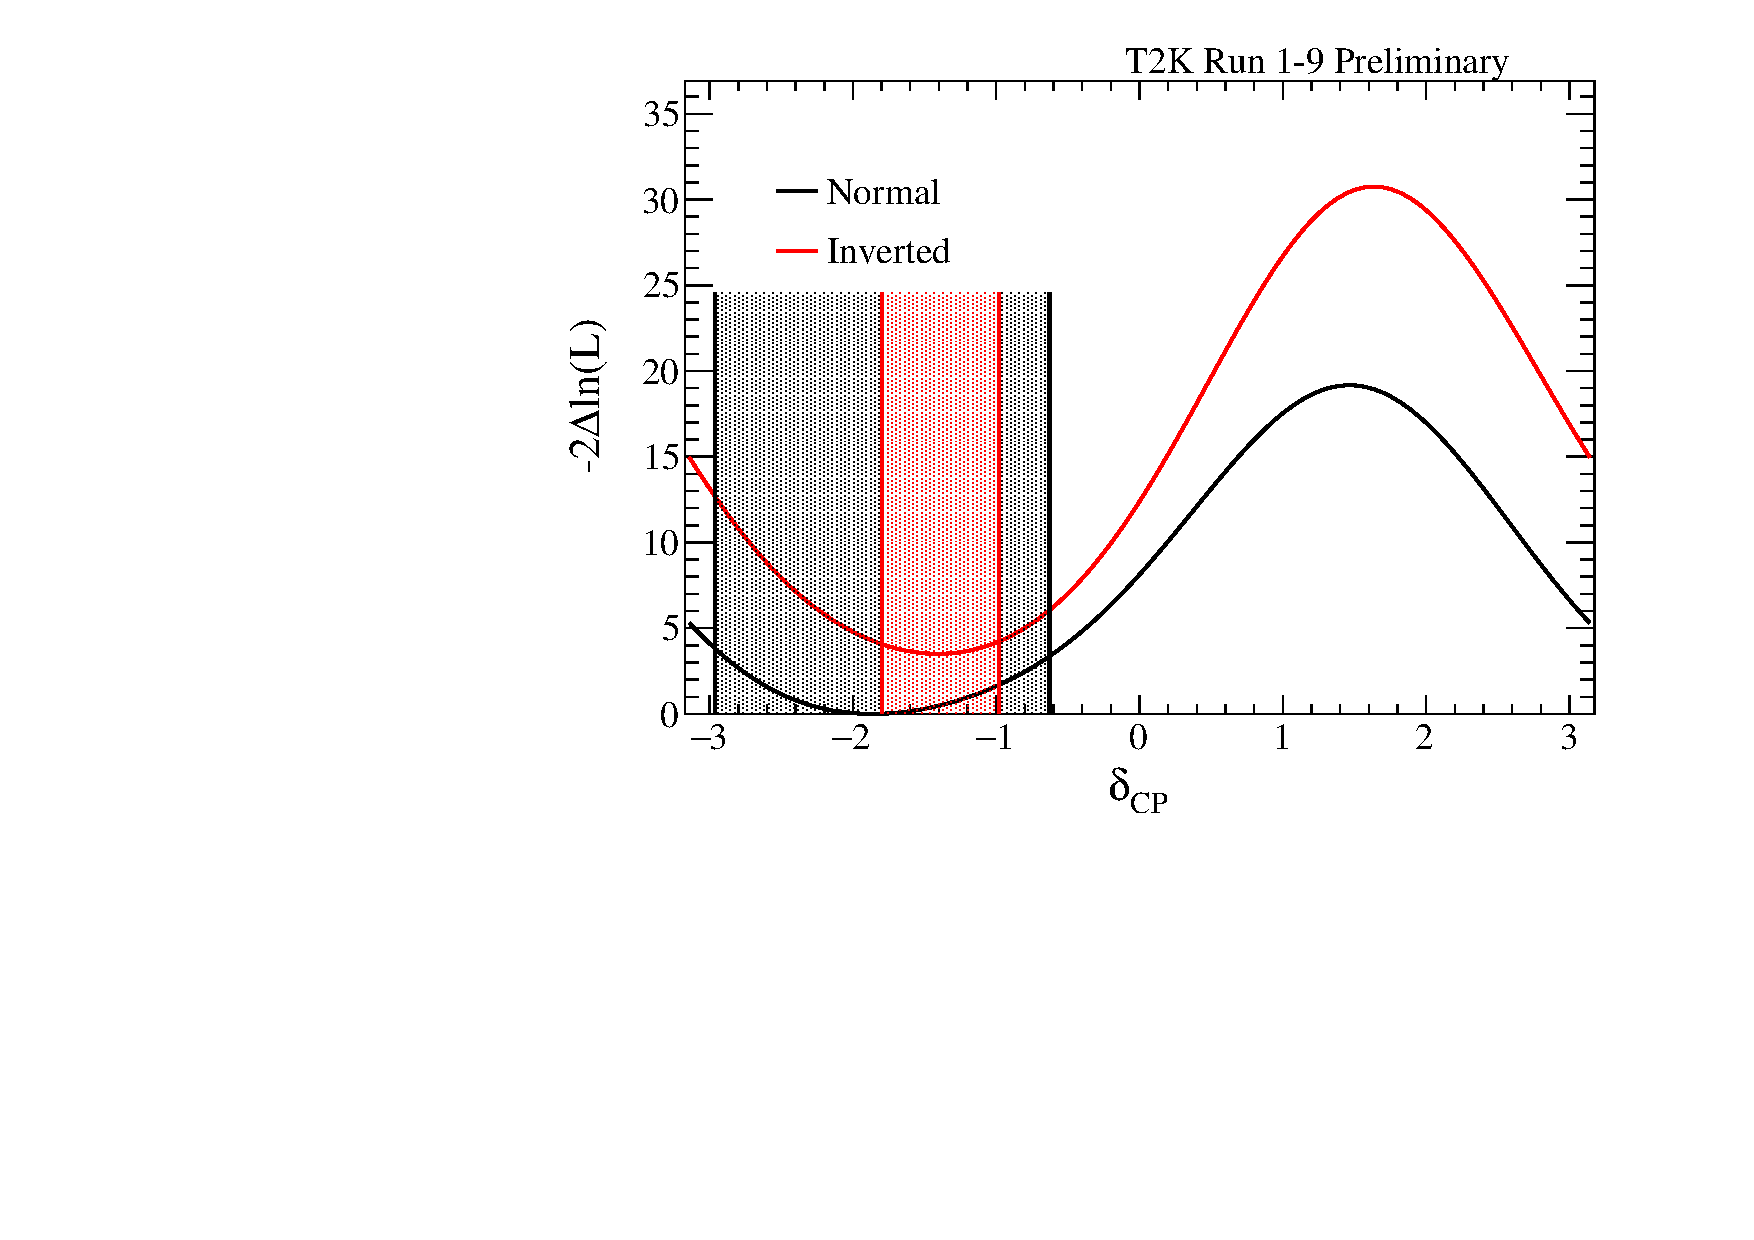
\includegraphics[width=0.9\textwidth]{images/fc/deltacp_mpi2_2sigma}
		\caption{$2\sigma$ CL exclusion region}
	\end{subfigure}
	\begin{subfigure}[b]{0.49\textwidth}
		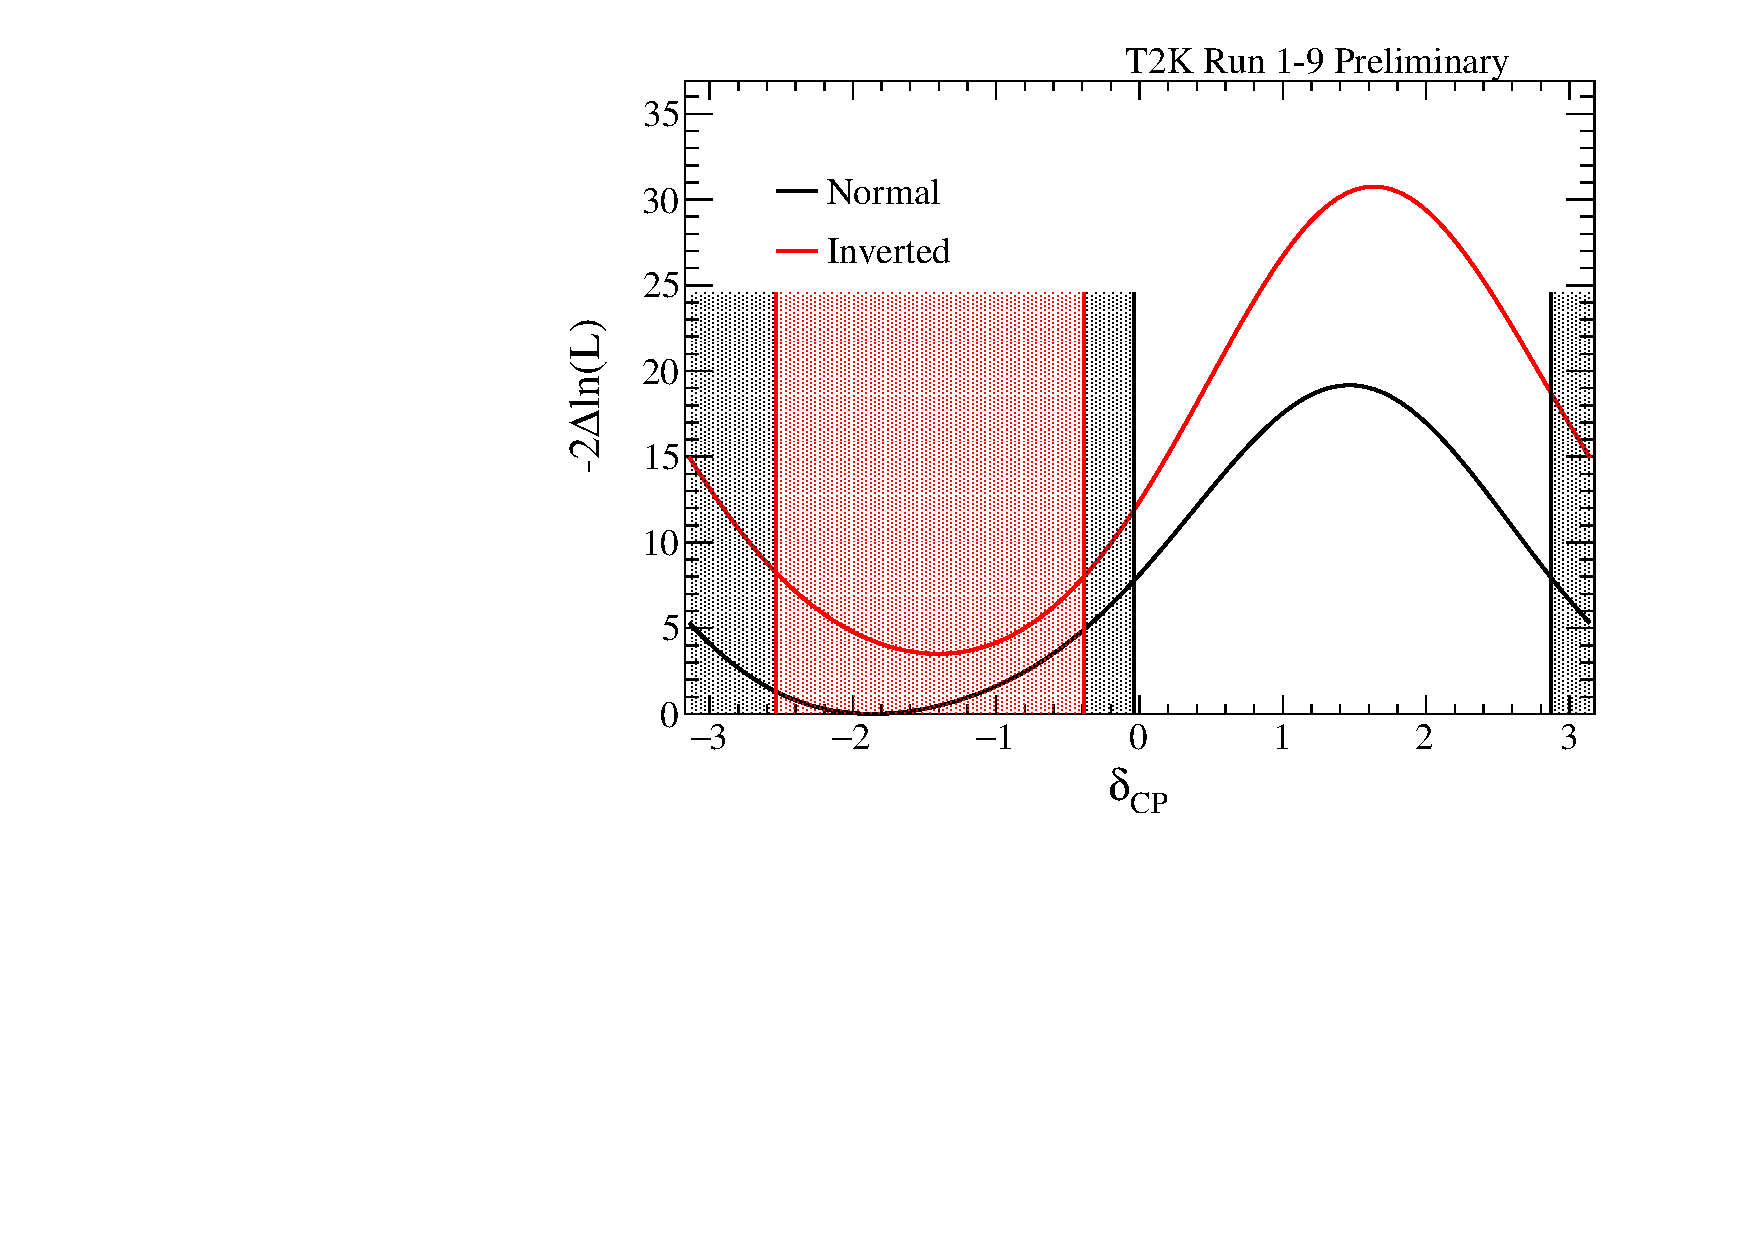
\includegraphics[width=0.9\textwidth]{images/fc/deltacp_mpi2_3sigma}
		\caption{$3\sigma$ CL exclusion region}
	\end{subfigure}
	\caption {
$\Delta\chi^2$ critical values and confidence intervals for the measured $\Delta\chi^2$ distributions for \RunPeriod. Critical values obtained with the Feldman-Cousins method for \RunPeriod for 9 evenly spaced values on the range \( \left[-\pi,\pi\right] \). Critical values are shown for 1\( \sigma \), 90\%, 2\( \sigma \) and 3\( \sigma \) CL for normal (solid lines) and inverted (dashed lines) hierarchies. At least \num{2e4} toy experiments are performed for each point. The three bands of lines show the \( \pm 1\sigma \) uncertainty on the critical values. Also shown are the measured \( \Delta \chi^2 \) distributions shifted with respect to the same global minium and the $1\sigma$, $2\sigma$ and $3\sigma$ exclusion regions for both mass hierarchies. 
	}
	\label{fig:fc_interval}
\end{figure*}

\begin{table}[htb]
	\centering
	\begin{tabular}{| c | c | c | c | c |}
\hline
Parameter & Reactor & CL & Normal hierarchy & Inverted hierarchy \\
\hline
\deltacp		& Yes & $ 1\sigma $ & $\left[ -2.510, -1.260 \right]$ & - \\
\deltacp		& Yes & 90\% & $\left[ -2.801, -0.844 \right]$ & - \\
\deltacp		& Yes & $ 2\sigma $ & $\left[ -2.965, -0.628 \right]$ & $\left[ -1.799, -0.979 \right]$ \\
\deltacp		& Yes & $ 3\sigma $ & $\left[ +2.874, -0.036 \right]$ & $\left[ -2.535, -0.389 \right]$ \\
\hline
\end{tabular}

	\caption{
		The confidence intervals at $1\sigma$, 90\%, $2\sigma$ and $3\sigma$ CL obtained with the Feldman-Cousins method for the \RunPeriod data set is shown for the measurement of \deltacp versus mass hierarchy.
	}
	\label{tab:fc_interval}
\end{table}

\FloatBarrier

\subsection {Discussion of the \RunPeriod data fit results}
\label{sec:results:discussion}

With no FHC running in 9d, the change in predicted FHC event rates comes from flux tuning bug fix noted in \ref{sec:intro}. The change in the prediction is small ($\sim1$\%) and results in a slightly larger difference between observed and Asimov A predicted rates in the one ring $\mu$-like sample, while the one ring $e$-like sample and \nueCConepi samples show a smaller difference between observed and Asimov A predicted rates. In summary, we continue to see an excess in the number of observed appearance events in the \nueCConepi data set (\NskObservedNueCConepi{})  compared to the Asimov A expectation (\NAsimovAExpectationNueCConepi{}), one ring $e$-like sample continues to show good agreement between observed (\NskObservedNue{}) and expected (\NAsimovAExpectationNue{}) events and we continue to see a deficit in observed (\NskObservedNumu{}) relative to expected (\NAsimovAExpectationNumu) events in the one ring $\mu$-like sample.

In RHC, where POT is increased by $\sim45$\%, we see improved agreement between observed (\NskObservedNueBar{}) and expected (\NAsimovAExpectationNueBar{}) events in the one-ring $e$-like sample, and between observed (\NskObservedNumuBar{}) and expected (\NAsimovAExpectationNumuBar) events in the one-ring $\mu$-like sample.

The value of \deltacp favoured by the joint fit analysis, when the reactor constraint is applied, is \BestFitDeltacpwRC (corresponding to normal hierarchy), close to $\delta_{CP} = -\pi / 2$ and rejects CP-conservation at the $2\sigma$ level when using the reactor constraint, both for the constant $\Delta\chi^2$ and the Feldman-Cousins methods. The new analysis excludes a slightly smaller range of values of $\delta_{CP}$ in normal hierarchy, relative to the previous analysis, while the allowed $2\sigma$ interval in inverted hierarchy has approximately doubled as a result of small increases in the critical $\Delta\chi^2$ values in combination with the flatness of the contour in the relevant region. If the reactor constraint is not applied, the best-fit value of \deltacp is \BestFitDeltacpwoRC (normal hierarchy).

The reactor appearance fit excludes CP-conservation at the 90\% level in normal hierarchy, whilst the value of \ssqthonethree in this 2D fit is in agreement with the PDG 2018 value at the $1\sigma$ level. For the T2K-only fit, a small region of the $1\sigma$ contour overlaps the PDG 2018 reactor constraint.

In the 1D fit, T2K favours a normal hierarchy best-fit value for \ssqthonethree of \BestFitMixingOneThreewoRC. Though the best-fit and $1\sigma$ interval remains largely unchanged from the previous analysis, the change in the reactor constraint means that the T2K-only fit is no longer in agreement with the reactor constraint at $1\sigma$, rather the agreement with the PDG 2018 value ($0.0212 \pm 0.0008$) is now $\sim1.3\sigma$ (see \cref{tab:data_bestfit}).

The value of \ssqthtwothree favoured by the analysis is \BestFitMixingTwoThreewRC (\BestFitMixingTwoThreewoRC) with (without) the reactor constraint and corresponds to normal hierarchy, with the 1D contours in agreement with and without the reactor constraint at $1 \sigma$, furthermore, the constraint is consistent with maximal mixing at the $1\sigma$ level, as seen in our previous analyses.

The value of \dmsqtwothree favoured by the analysis is \BestFitDmTwoThreewRC $\times 10^{-3}\text{ eV}^2\text{/c}^4$ (\BestFitDmTwoThreewoRC$\times 10^{-3}\text{ eV}^2\text{/c}^4$) with (without) the reactor constraint and corresponds to normal hierarchy, with the 1D contours in agreement with and without the reactor constraint at $1 \sigma$.

As with the previous analysis, we continue to see stronger constraints in data than expected from Asimov A sensitivity studies for \deltacp and \ssqthtwothree (see \cref{app:data_asimov_comparison}).

\subsection {Comparison of \deltacp versus mass hierarchy result with sensitivity}
\label{sec:results:brazilian}

In order to provide a better understanding of the results of the \RunPeriod data fit, the result has been compared with the expected sensitivity obtained from a large number (10k) of toy experiments for a true value of \deltacp, $-\pi/2$ and normal mass ordering. The method used to determine the expected sensitivity is described in section 5.9 of \cite{OurRun18JointAnalysis3Flavour}.

\subsubsection{$\delta_{CP} = -\pi/2$ - normal hierarchy}

In \cref{fig:brazilian_dcp_mpi2} the \RunPeriod data result for \deltacp versus mass hierarchy is compared to the $1\sigma$ and $2\sigma$ uncertainties on the $\Delta\chi^2$ distributions corresponding to $\delta_{CP} = -\pi/2$, the top row includes one-sided distributions, the middle row two-sided distributions, with normal hierarchy on the left and inverted hierarchy on the right. We see that the data contour is contained within the one-sided $2\sigma$ band for inverted hierarchy, whilst the data contour falls just outside the $2\sigma$ band for normal hierarchy in the region around $\delta_{CP} = 0$, whereas the data contour is contained within the two-sided $2\sigma$ band in both hierarchies.

We also see an interesting feature near $\delta_{CP} = -\pi/2$ where the $\Delta\chi^2$ values have a wider distribution. This is due to the boundary at $\delta_{CP} = -\pi/2$ which causes a wider distribution when the parameter \deltacp would like to be pushed beyond the boundary in the fit.

Finally from \cref{fig:brazilian_dcp_mpi2}(c) we see that $\delta_{CP} = 0$ and $\delta_{CP} = \pi$ are excluded at 90\% confidence level in around 46-48\% (see \cref{tab:exclusion_prob}) of the toy experiments and excluded at $2\sigma$ confidence level in 32-34\% of the toy experiments. Both CP-conserving values are excluded at the $2\sigma$ confidence level in about 25\% of the toy experiments.

\begin{figure*}[htb]
	\center
	\begin{subfigure}[b]{0.49\textwidth}
		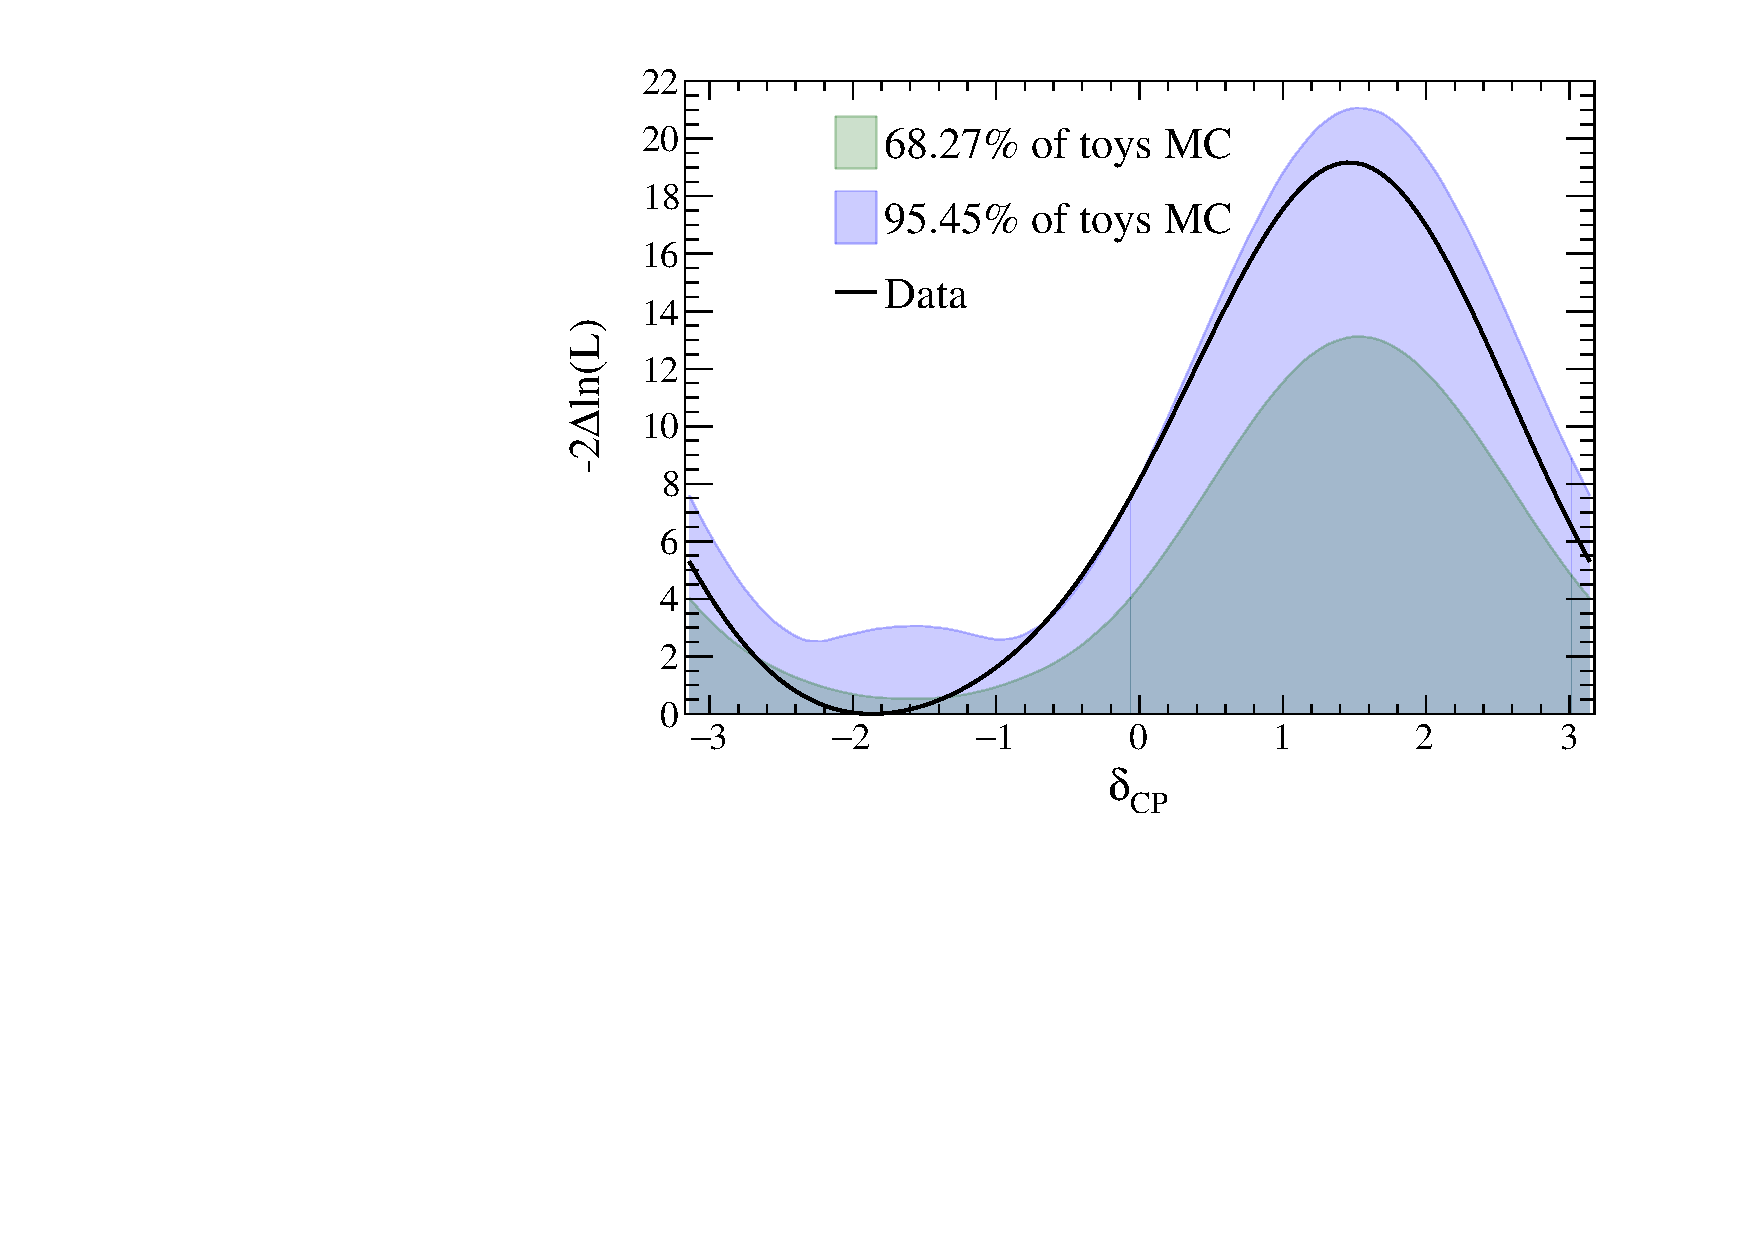
\includegraphics[width=0.9\textwidth]{images/fc/deltacp_mpi2_onesided_brazilian_nh}
		\caption{Normal hierarchy}
	\end{subfigure}
	\begin{subfigure}[b]{0.49\textwidth}
		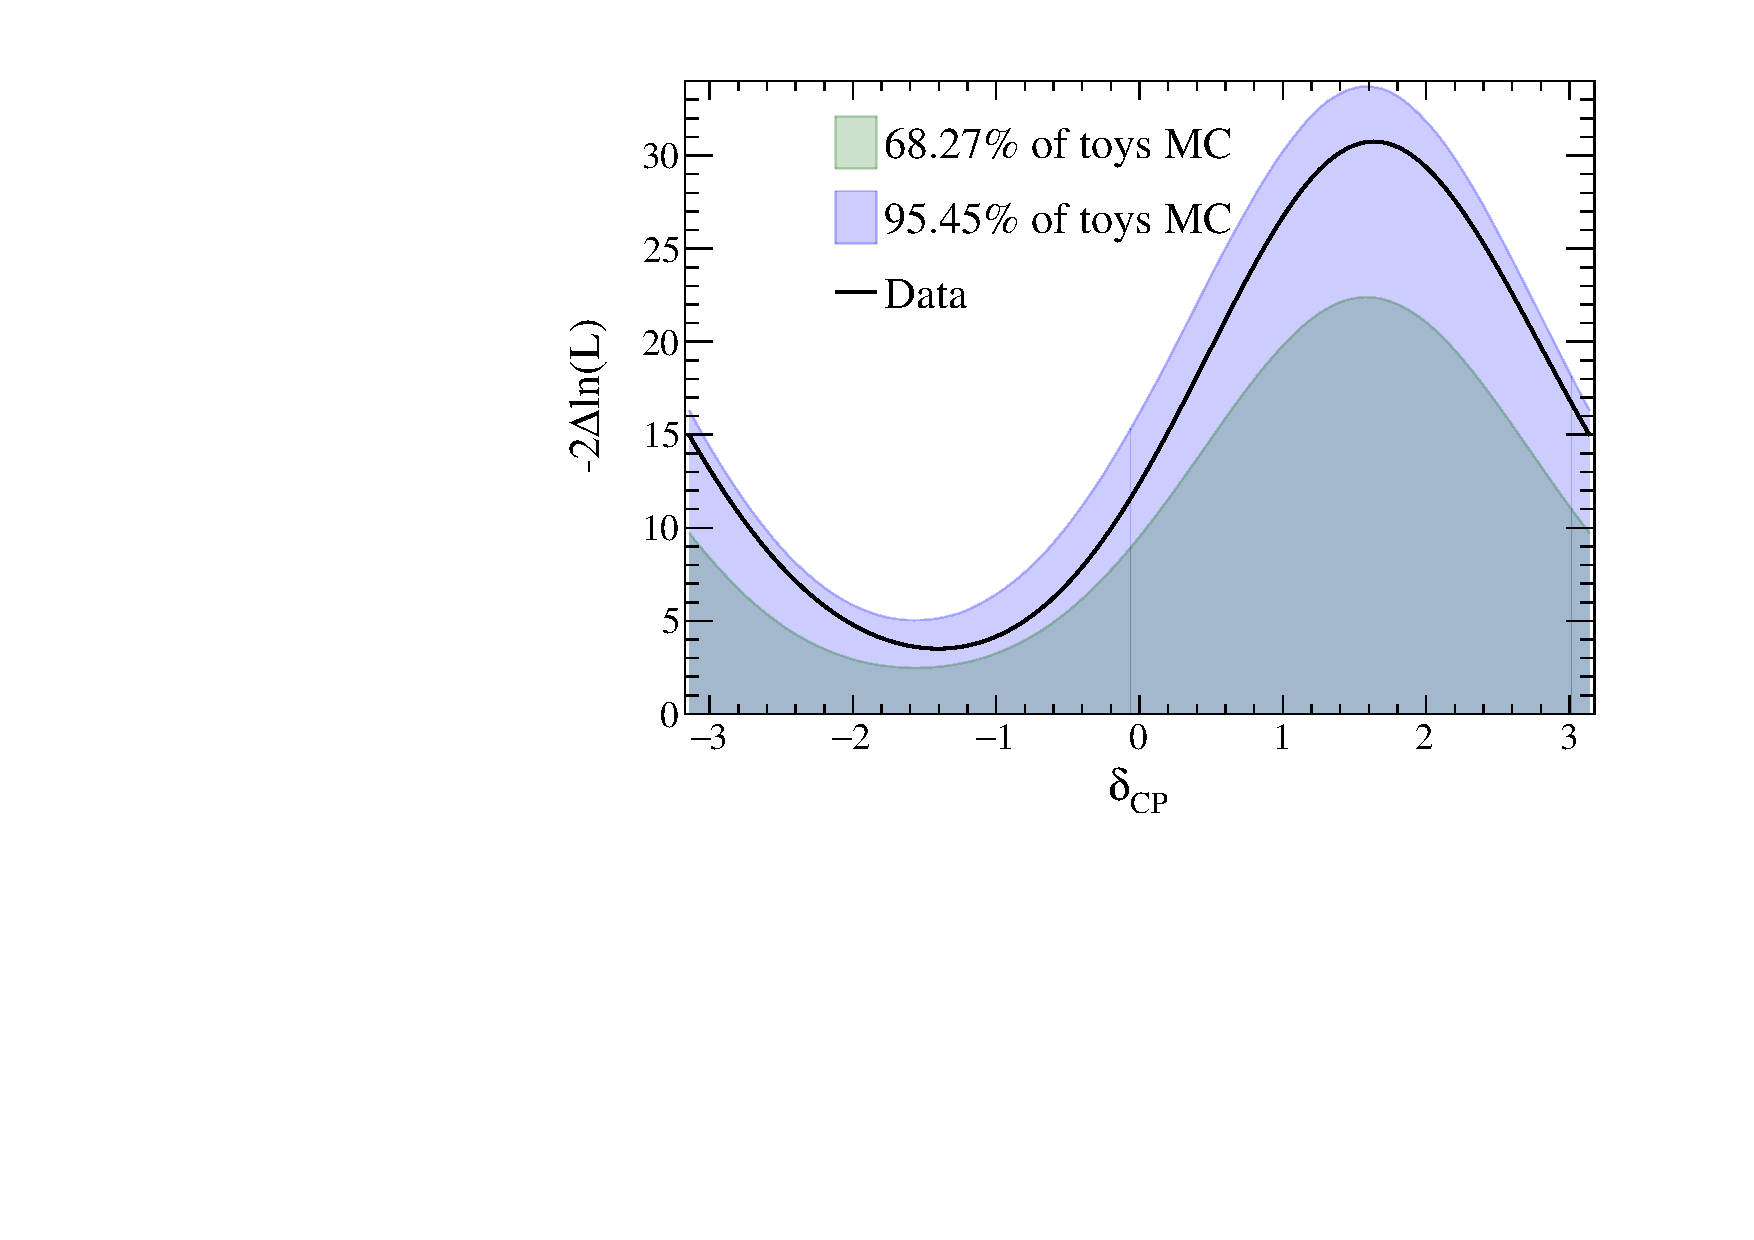
\includegraphics[width=0.9\textwidth]{images/fc/deltacp_mpi2_onesided_brazilian_ih}
		\caption{Inverted hierarchy}
	\end{subfigure}
	\begin{subfigure}[b]{0.49\textwidth}
		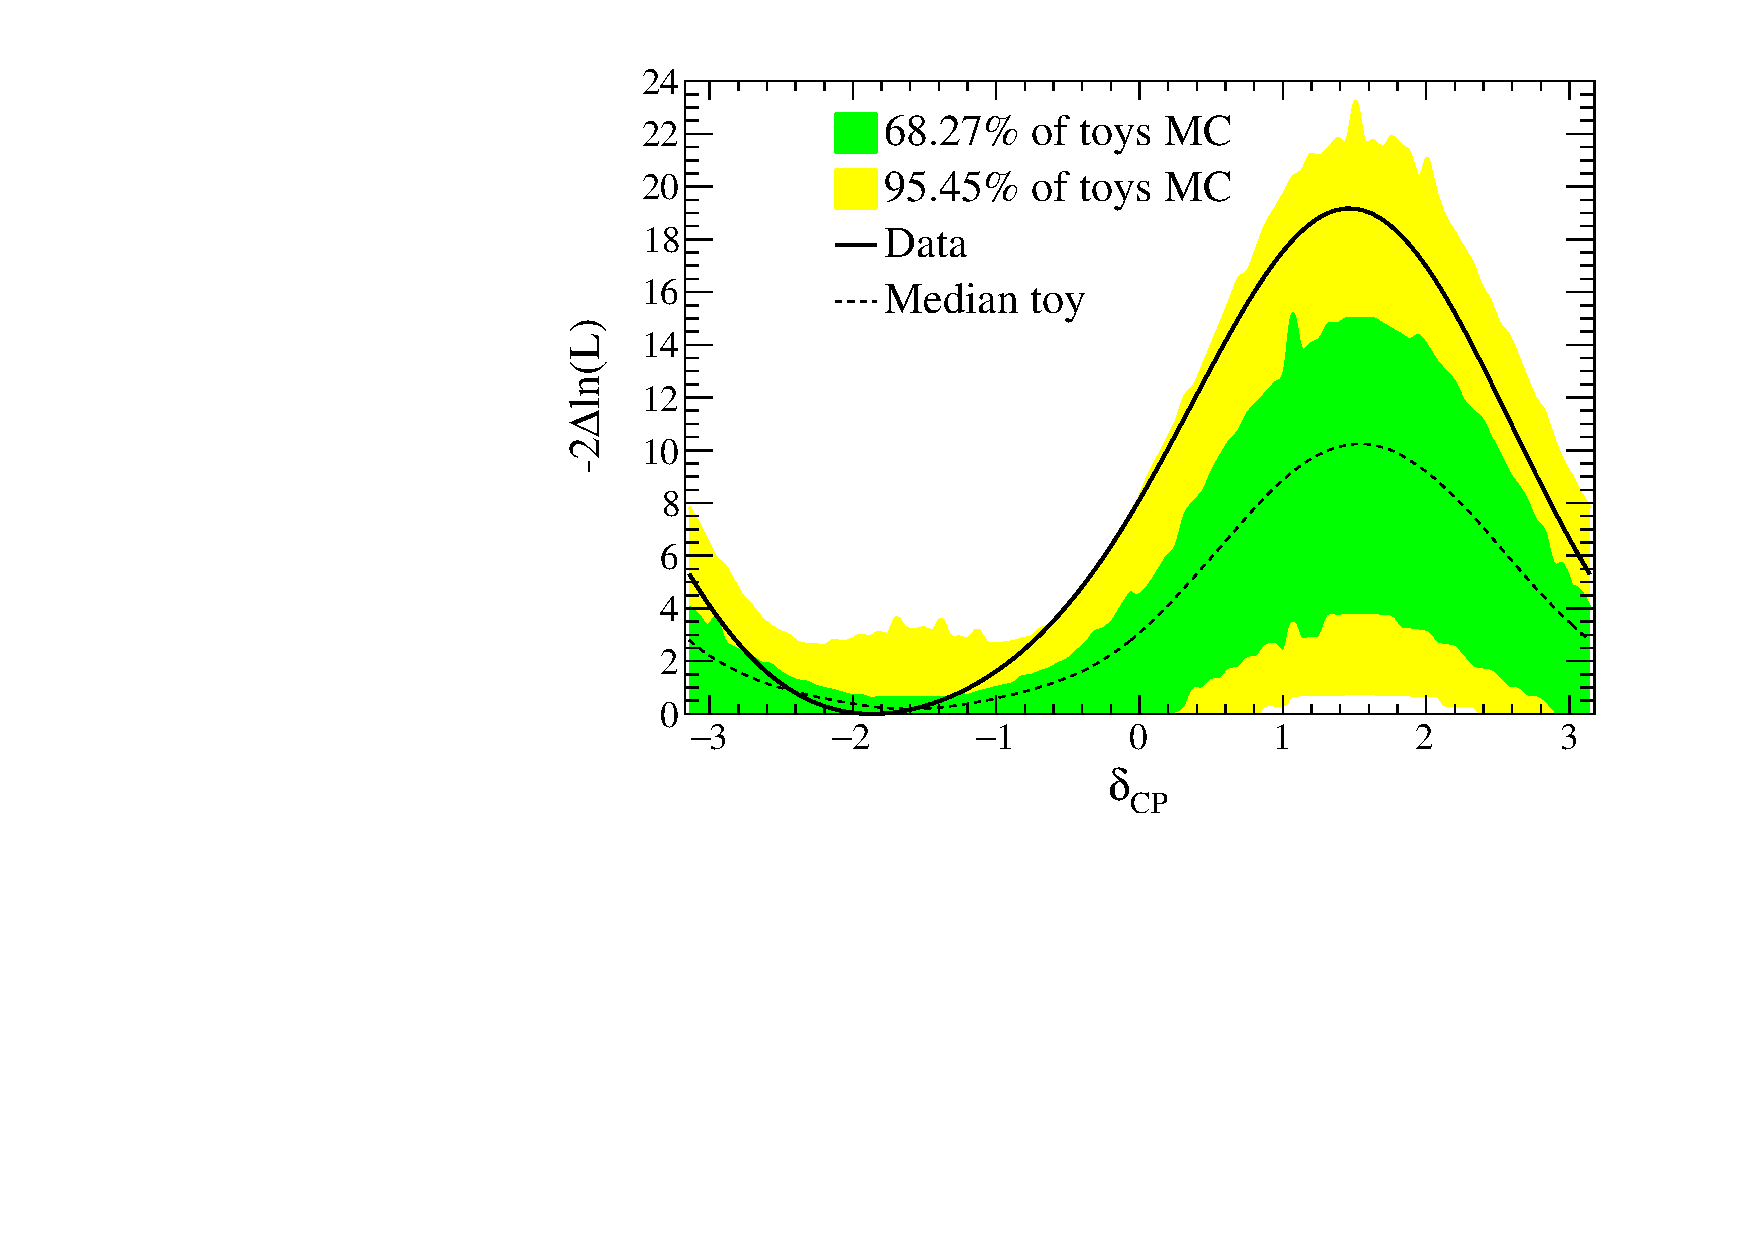
\includegraphics[width=0.9\textwidth]{images/fc/deltacp_mpi2_twosided_brazilian_nh}
		\caption{Normal hierarchy}
	\end{subfigure}
	\begin{subfigure}[b]{0.49\textwidth}
		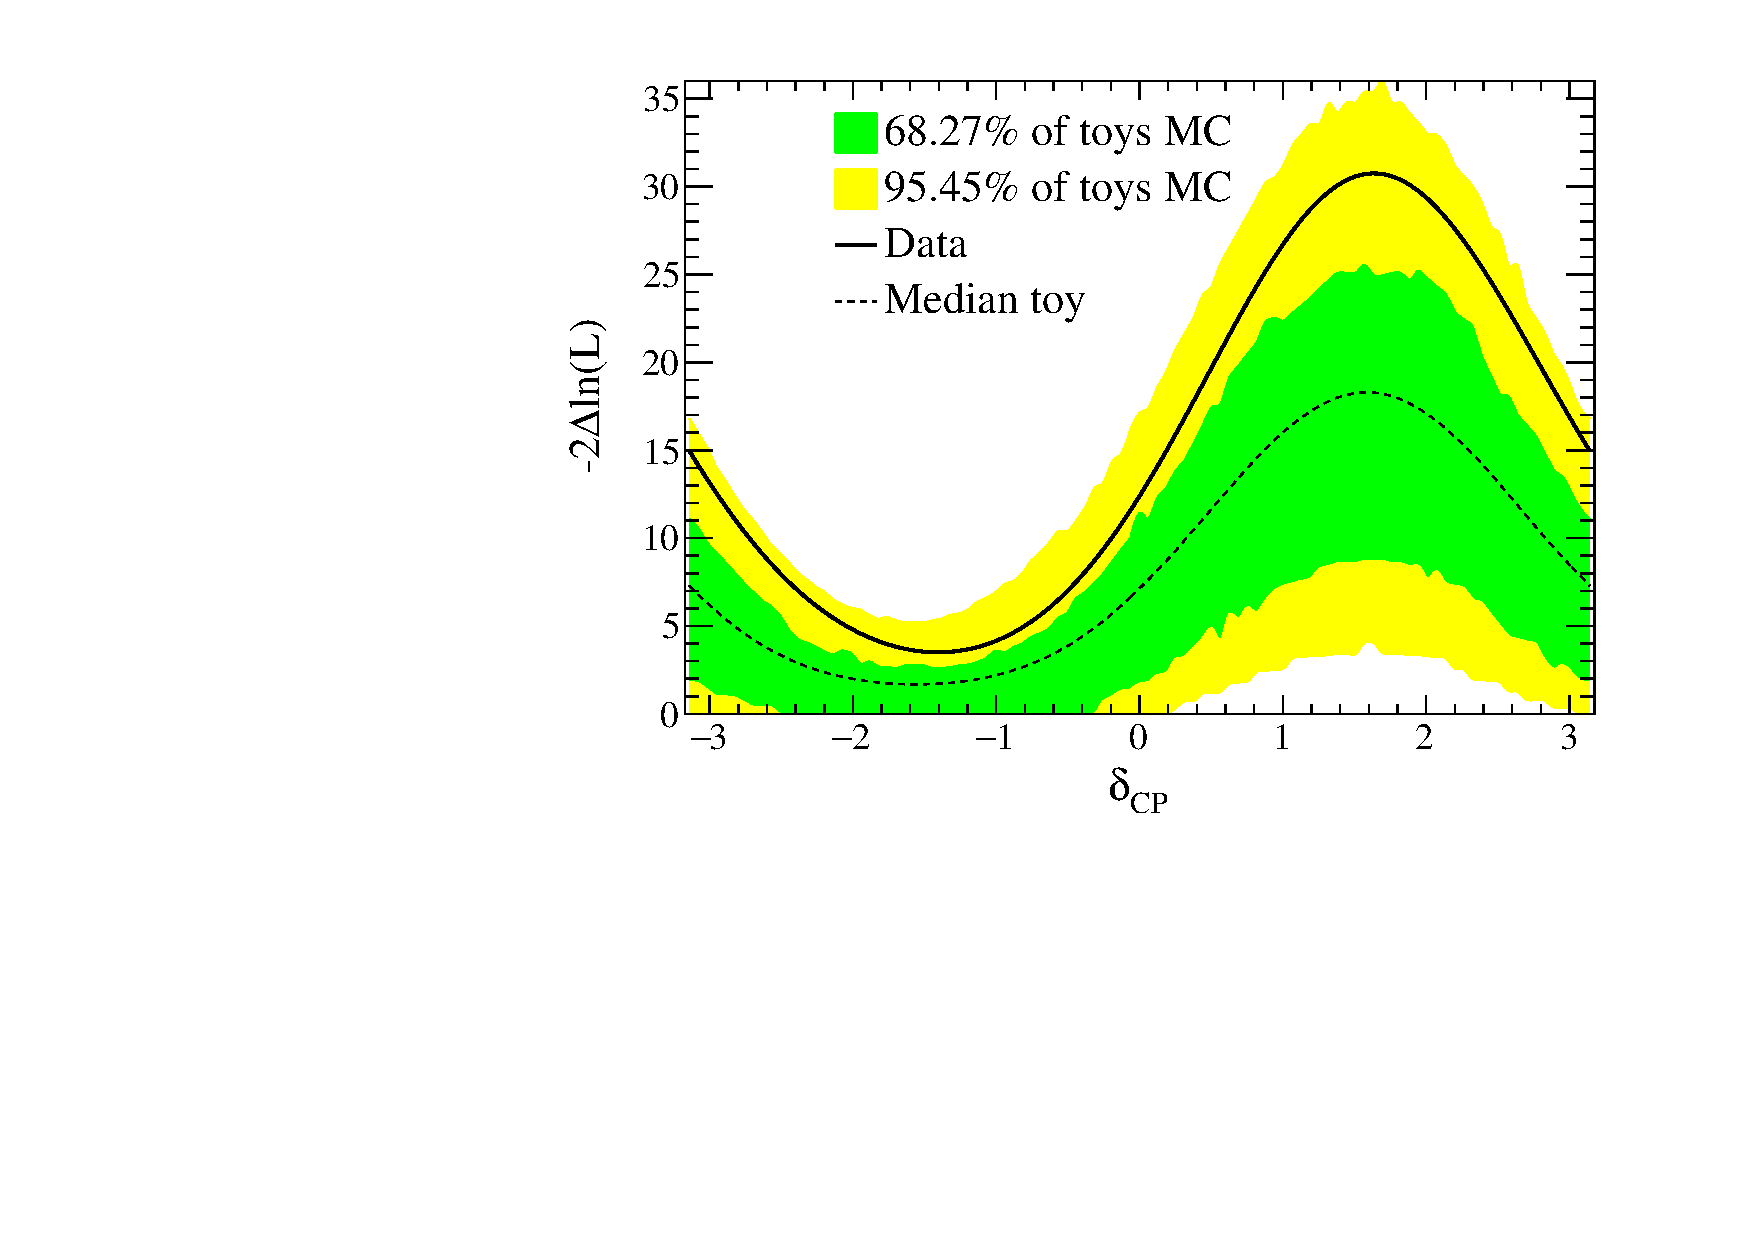
\includegraphics[width=0.9\textwidth]{images/fc/deltacp_mpi2_twosided_brazilian_ih}
		\caption{Inverted hierarchy}
	\end{subfigure}
	\begin{subfigure}[b]{0.49\textwidth}
		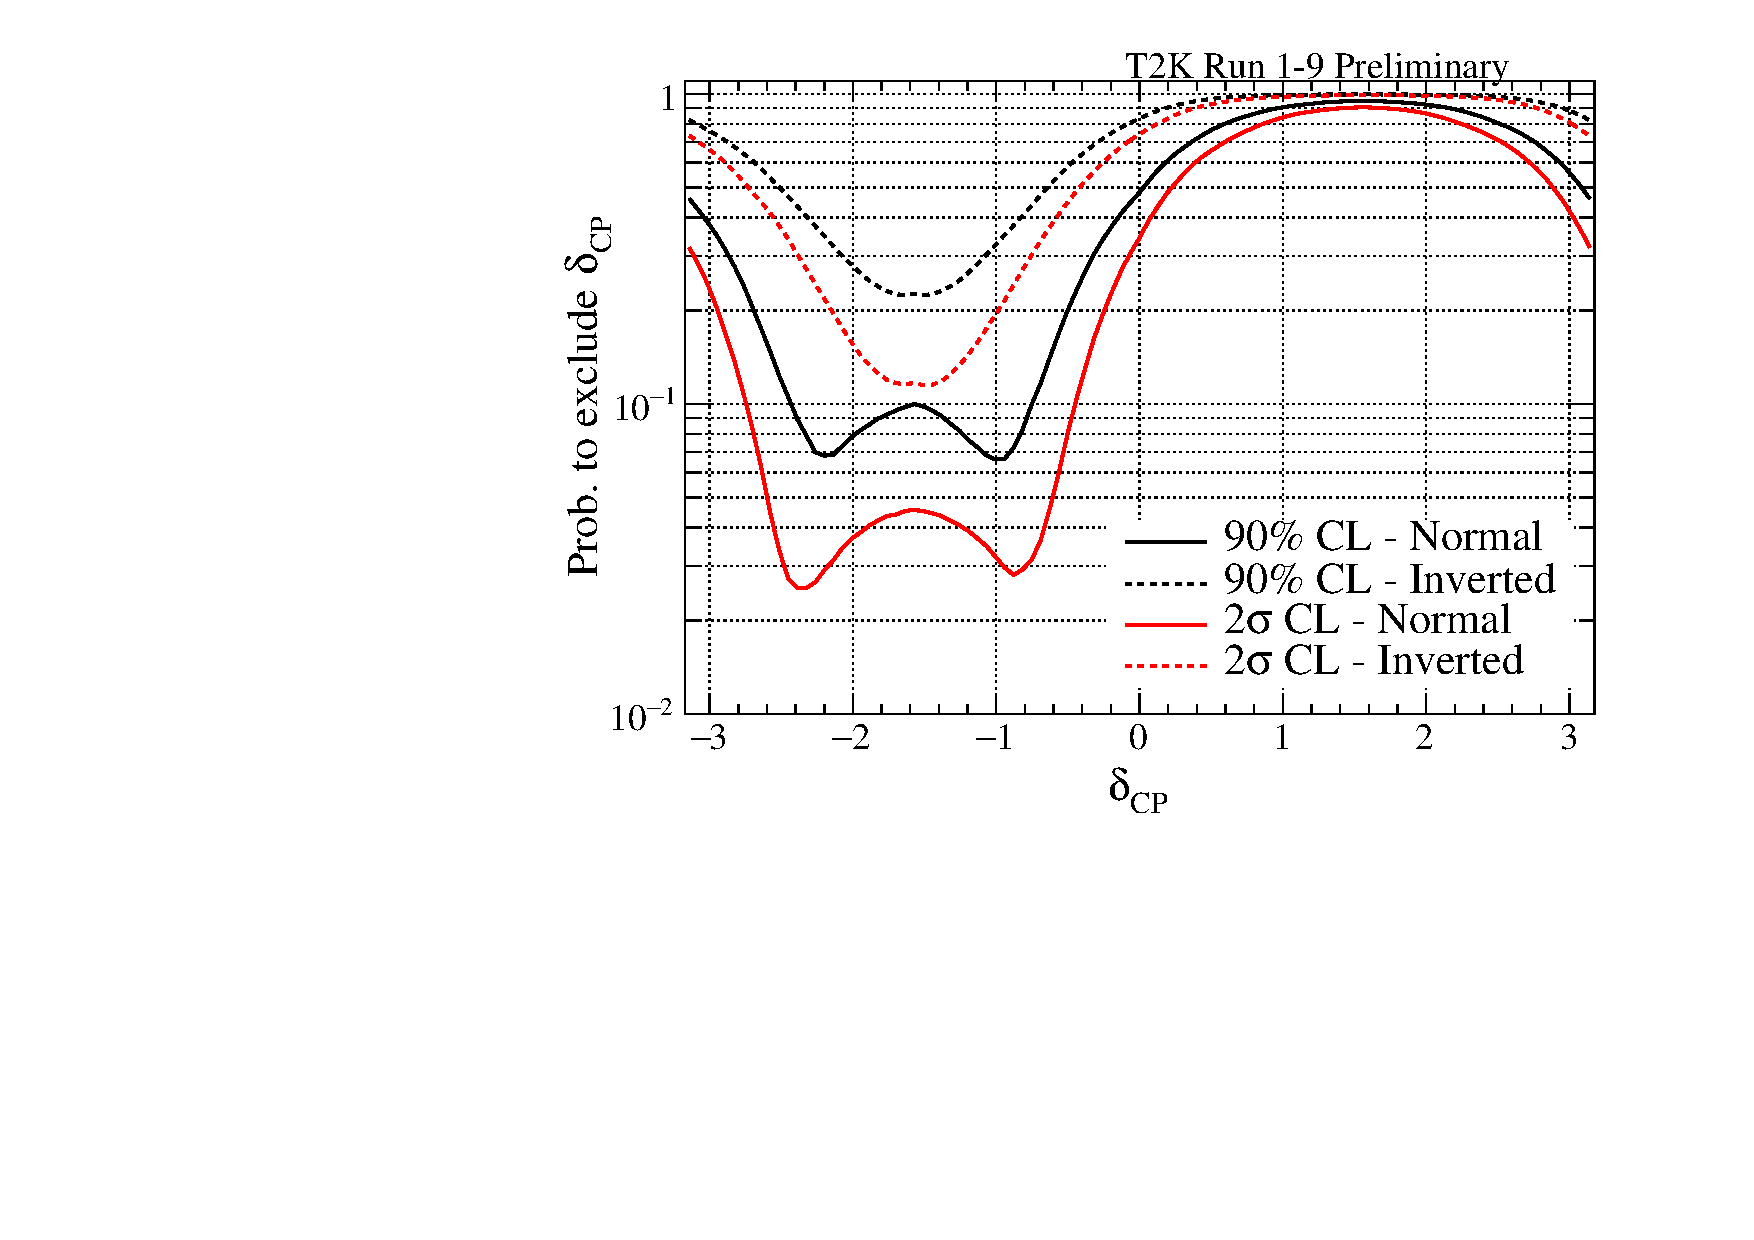
\includegraphics[width=0.9\textwidth]{images/fc/deltacp_mpi2_onesided_brazilian_prob_chisq}
		\caption{Data \(\Delta \chi^2\) probablility }
	\end{subfigure}
	\caption {
		The one-sided distribution of $\Delta\chi^2$ vs \deltacp obtained with \num{1e4} toy experiments generated with $\delta_{CP} = -\pi/2$ and normal hierarchy is shown. The $\Delta\chi^2$ distributions obtained by fixing the mass hierarchy to normal (left) and inverted (right) are shown, along with the $\Delta\chi^2$ values corresponding to 68.27\% and 95.45\% of the toy experiments and the average $\Delta\chi^2$ values from all experiments. Also shown are the fractions of toys which exclude each value of \deltacp to 90\% and $2\sigma$ using the Feldman-Cousins corrected critical values (bottom).
	}
	\label{fig:brazilian_dcp_mpi2}
\end{figure*}

\begin{table}[htb]
	\centering
	\begin{tabular}{| c | c | c | c |}
\hline
\deltacp & Hierarchy & 90\% & $2\sigma$ \\
\hline
0			& NH & 0.481 & 0.344 \\
$\pi$		& NH & 0.459 & 0.320 \\
0			& IH & 0.833 & 0.742 \\
$\pi$		& IH & 0.823 & 0.734 \\ \hline
0 and $\pi$	& NH & - & 0.249 \\
0 and $\pi$	& IH & - & 0.688 \\
\hline
\end{tabular}

	\caption{
		The fraction of toy experiments for which $\delta_{CP} = 0, \pi$ and normal and inverted hierarchy are excluded at 90\% and $2\sigma$ CL is shown. 10k toy experiments are used.
	}
	\label{tab:exclusion_prob}
\end{table}

\FloatBarrier
\iffalse
\subsubsection{$\delta_{CP} = -1.822$ - normal hierarchy}
\color{red}
In \cref{fig:brazilian_dcp_bf} the \RunPeriod data result for \deltacp versus mass hierarchy is compared to the $1\sigma$ and $2\sigma$ uncertainties on the $\Delta\chi^2$ distributions corresponding to $\delta_{CP} = -1.822$, the top row includes one-sided distributions, the middle row two-sided distributions, with normal hierarchy on the left and inverted hierarchy on the right. We see that the data contour is contained within the one-sided $2\sigma$ band for inverted hierarchy, whilst the data contour falls just outside the $2\sigma$ band for normal hierarchy in the region around $\delta_{CP} = 0$, whereas the data contour is contained within the two-sided $2\sigma$ band in both hierarchies.

Finally from \cref{fig:brazilian_dcp_bf}(c) we see that $\delta_{CP} = 0$ and $\delta_{CP} = \pi$ are excluded at 90\% confidence level in around 38-42\% (see \cref{tab:exclusion_prob}) of the toy experiments and excluded at $2\sigma$ confidence level in around 25-29\% of the toy experiments.

\begin{figure*}[htb]
	\center
	\begin{subfigure}[b]{0.49\textwidth}
%		\includegraphics[width=0.9\textwidth]{images/fc/deltacp_bestfit_onesided_brazilian_nh}
		\caption{Normal hierarchy}
	\end{subfigure}
	\begin{subfigure}[b]{0.49\textwidth}
%		\includegraphics[width=0.9\textwidth]{images/fc/deltacp_bestfit_onesided_brazilian_ih}
		\caption{Inverted hierarchy}
	\end{subfigure}
	\begin{subfigure}[b]{0.49\textwidth}
%		\includegraphics[width=0.9\textwidth]{images/fc/deltacp_bestfit_twosided_brazilian_nh}
		\caption{Normal hierarchy}
	\end{subfigure}
	\begin{subfigure}[b]{0.49\textwidth}
%		\includegraphics[width=0.9\textwidth]{images/fc/deltacp_bestfit_twosided_brazilian_ih}
		\caption{Inverted hierarchy}
	\end{subfigure}
	\begin{subfigure}[b]{0.49\textwidth}
%		\includegraphics[width=0.9\textwidth]{images/fc/deltacp_bestfit_onesided_brazilian_prob_chisq}
		\caption{Data \(\Delta \chi^2\) probablility }
	\end{subfigure}
	\caption {
		The one-sided distribution of $\Delta\chi^2$ vs \deltacp obtained with \num{1e4} toy experiments generated with $\delta_{CP} = -1.822$ and normal hierarchy is shown. The $\Delta\chi^2$ distributions obtained by fixing the mass hierarchy to normal (left) and inverted (right) are shown, along with the $\Delta\chi^2$ values corresponding to 68.27\% and 95.45\% of the toy experiments and the average $\Delta\chi^2$ values from all experiments. Also shown are the fractions of toys which exclude each value of \deltacp to 90\% and $2\sigma$ using the Feldman-Cousins corrected critical values (bottom).
	}
	\label{fig:brazilian_dcp_bf}
\end{figure*}

\begin{table}[htb]
	\centering
	\begin{tabular}{| c | c | c | c |}
\hline
\deltacp & Hierarchy & 90\% & $2\sigma$ \\
\hline
0		& NH & 0.421 & 0.288 \\
$\pi$	& NH & 0.388 & 0.248 \\
0		& IH & 0.768 & 0.660 \\
$\pi$	& IH & 0.783 & 0.685 \\
\hline
\end{tabular}

	\caption{
		The fraction of toy experiments for which $\delta_{CP} = 0, \pi$ and normal and inverted hierarchy are excluded at 90\% and $2\sigma$ CL is shown. 10k toy experiments are used.
	}
	\label{tab:exclusion_prob_bf}
\end{table}
\color{black}
\fi
\FloatBarrier

\subsection {Comparison of $e$-like event rates with expectation}
\label{sec:results:bievent}

It is valuable to see how different values of \deltacp, \ssqthtwothree and hierarchy affect the predicted event rates. \Cref{fig:bievent} shows the predicted $\nueb$ event rate vs $\nue$ event rate for best-fit values of oscillation parameters where \deltacp is varied between CP conserving and maximally CP violating values, and \ssqthtwothree is varied around its best-fit, for both hierarchies. Event rates for a given value of \ssqthtwothree and mass hierarchy are linearly interpolated between those computed for 9 evenly-spaced values of \deltacp from $-\pi$ to $+\pi$ to indicate the behaviour produced by varying \deltacp.

\begin{figure*}[htb]
	\centering
	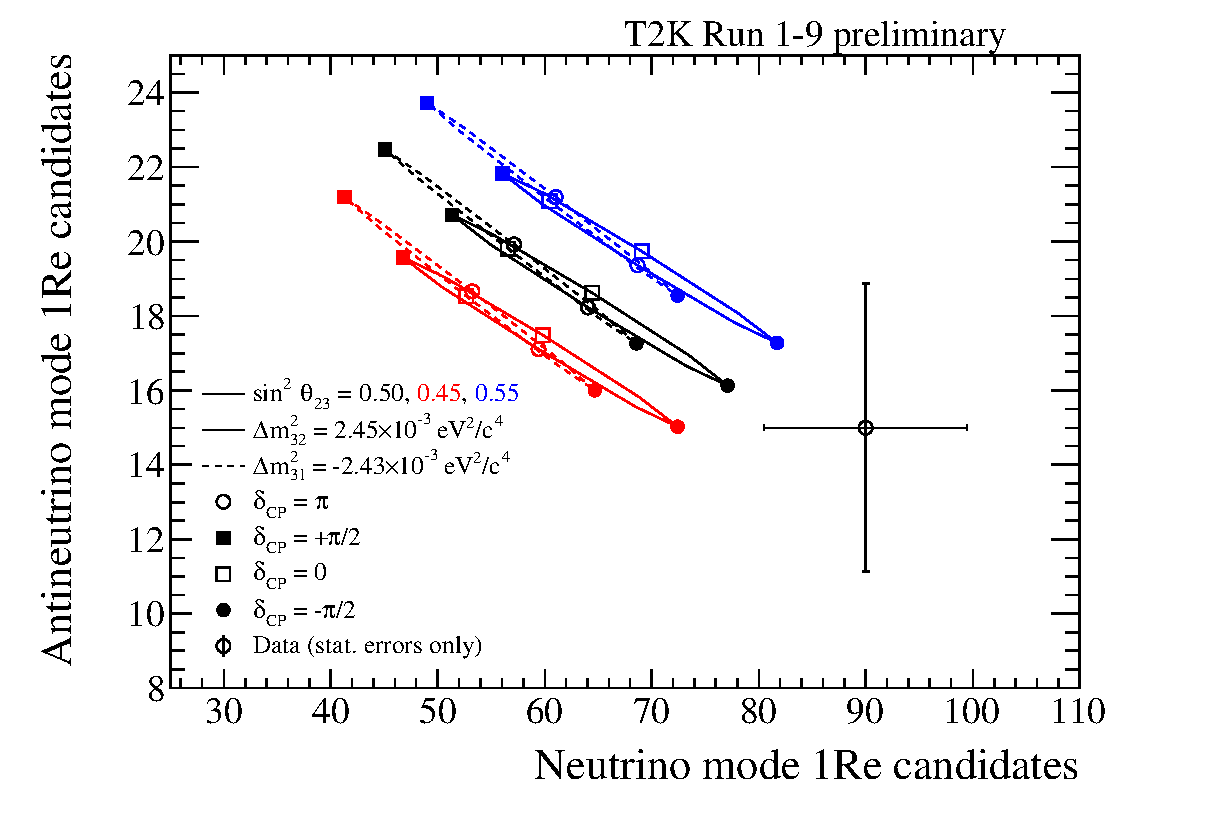
\includegraphics[width=0.7\textwidth]{images/bievent/ellipse_cc1pi_all}
	\caption {
		This plot shows the candidate RHC one-ring $e$-like event rate vs the candidate FHC one-ring $e$-like event rate for a variety of different oscillation parameter values. Predictions are generated for the given values of \deltacp, \ssqthtwothree and mass hierarchy with remaining oscillation parameters fixed at the central values defined in \cref{tab:osc_param_priors}.
	}
	\label{fig:bievent}
\end{figure*}

\clearpage
